\documentclass{umthesis}   



%% umd requirements 
%% use 11 or 12 pt font
%% chapter headings shouldnt be over 14 pt font

%% begin new chapters on a new page

%% no new heading on the bottom of a page unless there is room for at least two lines following the heading
%% left margin >= 1.5 inches
%% other margings == 1 inch


\usepackage[table]{xcolor}

\usepackage{titlesec} % included to typset the appendicies vertically centered


\usepackage[title,titletoc]{appendix}
%\usepackage{appendix}

\usepackage{tabularx}
\usepackage{graphicx}
\usepackage{subcaption}

\usepackage{import}
\usepackage{amsmath}

\usepackage{tocloft}

% %manual placement of figures via[h]
\usepackage{float}


\usepackage{sectsty}

%used to include documents in the apendix (IRB approval)
\usepackage{pdfpages}


%min bottom is 1.0in, i added an 1/8" to keep people happy
%same with left, min=1.5, i added an 1/8"
\usepackage[letterpaper,top=1.0in, bottom=1.125in,left=1.675in, right=1.0in, includefoot, includehead] {geometry}

\usepackage{calc}


% use showframe to check your margins and borders.
%\usepackage{showframe}



%use this package for printing hard copies
\usepackage[colorlinks,allcolors=black,]{hyperref}

%use this package for pdf publication
%\usepackage[colorlinks]{hyperref}
%use this package to easily find all links in a pdf
%\usepackage{hyperref}

% for source code listings
% \begin{lstlisting}
% Put your code here.
% \end{lstlisting}
%
%https://en.wikibooks.org/wiki/LaTeX/Source_Code_Listings
\usepackage{listings}
\lstset{language=C,
                basicstyle=\ttfamily,
                keywordstyle=\color{blue}\ttfamily,
                stringstyle=\color{red}\ttfamily,
                commentstyle=\color{green}\ttfamily,
                morecomment=[l][\color{magenta}]{\#}
}

\usepackage[all]{hypcap} % hyperlinks goto top of figures, not the bottom
\usepackage[capitalise,noabbrev,nameinlink]{cleveref}		% now \cref yields Figure 1.1 instead of 1.1 alone



\cftsetindents{chapter}{0em}{2em}
\cftsetindents{section}{1em}{2em}
\cftsetindents{subsection}{2em}{2em}
\cftsetindents{subsubsection}{3em}{2em}
\cftsetindents{paragraph}{4em}{2em}
\cftsetindents{fig}{0em}{3em}

\renewcommand{\cftchapaftersnum}{:}

\renewcommand{\cftchappresnum}{\chaptername\space} %adds 'Chapter ' to the TOC
\renewcommand{\cftchapfont}{\mdseries}
\renewcommand{\cftchappagefont}{\mdseries}
\setlength{\cftchapnumwidth}{\widthof{\textbf{\chaptername~999~}}}
\setlength{\cftsecnumwidth}{\widthof{\textbf{~9.9~}}}
\setlength{\cftsubsecnumwidth}{\widthof{\textbf{~9.9.99~}}}
\setlength{\cftsubsubsecnumwidth}{\widthof{\textbf{~9.9.99.9~}}}
%\renewcommand{\cftchapleader}{\cftdotfill{\cftdotsep}} % chapters dont get dot leaders

%this adds the word Appendix to the Table of contents entries
\makeatletter
\g@addto@macro\appendix{%
  \addtocontents{toc}{%
    \protect\renewcommand{\protect\cftchappresnum}{}%
    \setlength{\cftchapnumwidth}{\widthof{\textbf{~9~}}}
  }%
}
\makeatother


\chapterfont{\centering}


\setlength{\emergencystretch}{4pt}



\newcommand{\apendixStyle}{
\titleformat{\chapter} %command
[display] %shape
{\bfseries\huge} % fromat
{\vfill\centering\chaptertitlename\ \thechapter} %label
{2pt} %sep
{
\centering 
} %beforecode
[
\vfill
\clearpage
] %aftercode

\titleformat{\section} %command
[hang] %shape
{\bfseries\large} % fromat
{\chaptertitlename\ \thesection} %label
{2pt} %sep
{
} %beforecode
[
] %aftercode
\titlespacing*{\chapter}{0pt}{0in}{0in}
\titlespacing*{\section}{0pt}{0in}{0in}
}




\begin{document}

%%
%% You must fill in all of these appropriately
\title{Wireless Health Indicator Patch  for Patient Education and Diagnostics (WHIPPED): \linebreak[1] An Integrated System Approach to Patient Self-Care}

\author{Benjamin Roy Viall}
\date{January 2017} % The date you'll actually graduate -- must be
                     % January, May, or September
\copyrightyear{2017}
\school {University of Massachusetts Dartmouth} 
\bachelors{B.Sc.}{University of Massachusetts Dartmouth} % where you got your bachelors
\masters{M.Sc.}{University of Massachusetts Dartmouth} % where you got your masters

\degree{Doctor of Philosophy}{Ph.D.} % what degree type and abreviation
\degreeTitle{Computer Engineering} % what is your degree in

%\committeechair{Paul Fortier}{Professor, Department of Computer Engineering}{Dissertation Advisor}
\committeechair{Paul Fortier}{Professor}{Computer Engineering}

\firstreader{Honggang Wang}{Associate Professor}{Computer Engineering}
\secondreader{Liudong Xing}{Professor}{Computer Engineering}
\thirdreader{Kristen Sethares}{Professor}{Adult Nursing}

\fourthreader{Janet Prichard}{Professor}{Computer Information Systems \linebreak[1] Bryant University, Rhode Island}


\graduatedirector {Hong Liu}
\chairperson [Chairperson]{Antonio H. Costa}
\dean [Dean, College of Engineering] {Robert Peck} 
\provost {Tesfay Meressi}

%\departmentchair{Dr. Anthony Costa} % Uses "Department Chair" as the title. To
% use an alternate title, such as "Chair", use \departmentchair[Chair]{Pete Shearer}

\departmentname{Electrical and Computer Engineering}




%% start document with the basic bullshit that people pick over with a fine tooth comb
\frontmatter

\newgeometry{top=1.5in, bottom=1.5in,left=1.5in, right=1.5in}
\maketitle
\restoregeometry


\permissionpage
%%\copyrightpage     %% not required for an M.S. thesis
\newgeometry{top=1in, bottom=1in,left=1.675in, right=1.0in}
\signaturepage
\restoregeometry


%%
%% Abstract is MANDATORY. -- Except for MS theses
%%
%% Abstract is MANDATORY. -- Except for MS theses
\begin{abstract}                % Abstract
  Chronic Heart Failure (CHF) is a complex malady caused by numerous disorders of the heart and body resulting in a decreased quality of life. Care for current cardiac patients, post-hospitalization, is not uniform often resulting in relapses and early death. Despite the emergence of numerous therapeutic innovations, prolonging life and shorten hospital stays, CHF patients often have poor prognosis. Monitoring and involving the patient in self-care has been shown to improve upon the prognosis. We propose a new and novel system for cardiac heart failure patient's self-care. This system will collect both physiologic and psychosocial data from the patient using a combination of a custom sensor suite and a smartphone. An exploratory trial evaluates the effectiveness of such an approach.
  
  blank
  
  Review and Comment Received 10/11/2016
  \begin{itemize}
  \item Do not use 1st person e.g. I,me, etc.
  \item get rid of prepositions, starting sentences in particular!
  \item this helps \begin{verbatim}
	[\.!?][ ]?(of|in|to|for|with|on|at|from|by|about|as|into|like|through|after|over|between)[ ]([^\.!?]*[\.!?])
  \end{verbatim}
   \item  this, it, that, etc. replace with noun.
  \item make sure tense is consistent. youre writing about a completed piece of work so use past tense as appropriate.
  \item s/will be/..../
  \item s/will/
  \item check required format for references. if IEEE +[\#] then make sure you put references in \underline{\underline{order}} of use in dissertation.
  \item Trials - you need to beef up this section. describe all things that occurred what ??? found out from data. if anything, what could be done differently, time, issues, etc.
  \item Conclusion - restate what your dissertation contributions are.
  
  \item /s/shows/indicates/
  \item \Cref{sec:ResearchDoneToDate} <- need updating, should i make this into another chapter and redo the entire section in the past tense?
  \item our -> 'the' or 'the dissertation's' or 'the WHIPPED' or ''[sic]
  
  \item Show a calculation using the measured ECG and PPG trace to be uniform with your other descriptions. %great just what i wanted to do %
  
  \end{itemize}

  
\end{abstract}


%
%\begin{dedication}              % Dedication page
%  \begin{center}
    
%  \end{center}
%\end{dedication}


%% Acknowledgements are optional...yeah, right.
\phantomsection
\chapter*{Acknowledgments}             % Acknowledgements page
	\begin{center}
	\emph{Dedicated to Ken And Laura Viall, \\ who showed, by example, \\ how to be the kind of person I could be proud of.}
	\end{center}
  
  \parskip
  \parskip
  
  I would like to acknowledge the following individuals, without whom, this research would not have been possible. Dr. Fortier, my dissertation advisor, mentor, and friend who first recruited me into pursuing a PhD. Dr. Sethares, for her patience and for taking the time to educate me on all matters medical. My committee, whose doors have always been open anytime I needed advice. Gwen Davis who worked with me in creating the smartphone application and continued to support the study long after the funding ran out. Finally, to Professor Phil Viall, who has been my teacher in life, and engineering, for longer than I can remember. 
  
  I would also like to acknowledge the support of the Institutional Research Board (IRB) in approving the exploratory study at the core of this dissertation, and the funding of the University of Massachusetts Dartmouth bridge grant.

%%% option to show the table of contents with the hyper ref package.
\cleardoublepage
\phantomsection

%% this should be removed before submitting to the graduate studies office
%\addcontentsline{toc}{chapter}{\contentsname}
%% this should be removed before submitting to the graduate studies office.



\clearpage
\tableofcontents				 % table of contents
\clearpage
\phantomsection
\addcontentsline{toc}{chapter}{List of Figures}
%\chapter{List of Figures}
\listoffigures                  % List of Figures
%clearpage
%\listoftables                   % List of Tables



%% Time for the body of the dissertation
\mainmatter   %% <-- This line is mandatory for the umd thesis class



%pdf bookmarks cant have funny characters so we define alternative forms here.
\def \spo2{ \texorpdfstring{SpO$_{2}$}{SpO2}}
\def \nospacespo2{\texorpdfstring{SpO$_{2}$}{SpO2}}


%% stuff goes HERE
%optionally left justify (umass only allows full justification when using latex...whatever.)
%\raggedright
%\parindent=1.5em

\chapter{Introduction}
\label{chap:introduction}
%In the Introduction chapter, I will discuss the current state of medical care for CHF patients. I will present the relevant statistics about hospitalization and mortality. I will then cover the topic of engaging patients in their own self-care, citing relevant studies and statistics. Then finally indicate my proposed solution.


\begin{figure}[ht]

	\begin{center}

		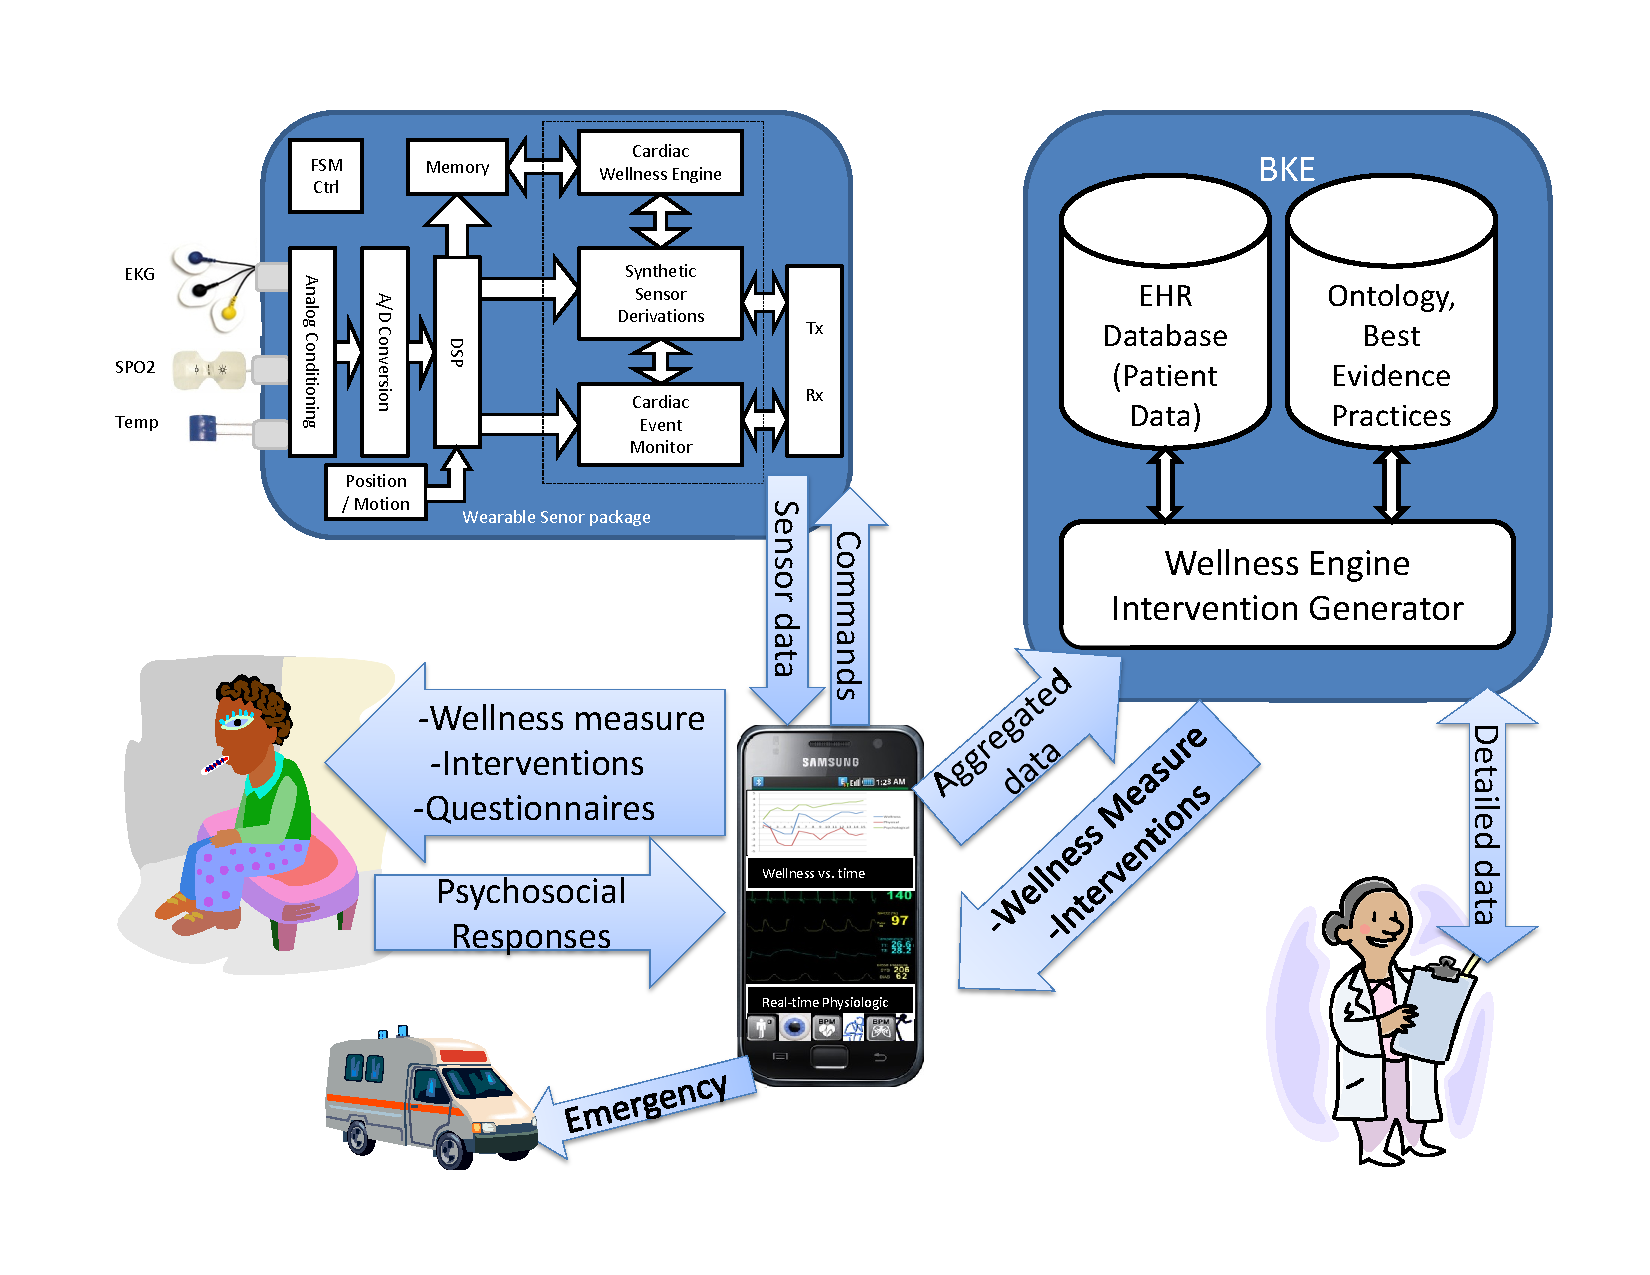
\includegraphics[scale=1,width=0.8  \textwidth]{Images/SystemConcept1.pdf} 
		\caption{WHIPPED System Design}
		\label{fig:WhippedSystem}
	\end{center}
\end{figure}

In \Cref{fig:WhippedSystem} we present a new and novel approach to chronic heart failure (CHF) outpatient care called the Wireless Health Indicator Patch for Patient Education and Diagnostics (WHIPPED). CHF is a complex malady caused by numerous disorders of the heart and body resulting in a decreased quality of life (QOL). Care for current cardiac patients, post-hospitalization, is not uniform often resulting in relapses and early death. Despite the emergence of numerous therapeutic innovations, to prolong life and shorten hospital stays, CHF patients often have poor prognosis. Monitoring and involving the patient in self-care can improve upon the prognosis.

This dissertation proposes a new and novel system for cardiac heart failure patient's self-care.  Self-Care encourages an individual to engage in healthy behaviors using targeted educational content. The WHIPPED system  wirelessly collects both physiologic and psychosocial data from the patient using a combination of a custom sensor suite and a smartphone. The collected data is sent to a back-end knowledge engine (BKE) and a wellness measure is calculated by the BKE. Both patient and clinician can access the wellness-score as well as wellness-history. The clinician can, in addition, view the raw data collected by the sensor suite and smartphone. The BKE also analyzes the collected data and offer interventions to patient whose wellness is not improving; reminding a patient to reduce salt or to increase activity levels, for example. Clinicians are also able to interact with the patient if needed. Both types of interactions are available through the patient's smartphone. Lastly, the system can contact emergency services if the patient is suffering from an exacerbation of a cardiac event.  

The WHIPPED system is split into three parts: an integrated mobile sensor platform (WHIP), a smartphone application, and a BKE. A wearable sensor patch collects physiologic readings from the patient using a combination of real and synthetically derived sensors and transmit them to the cell-phone. The cell-phone is used to prompt the patient to answer questions in order to gather psychosocial and symptom data concerning the perceived state of the patient, and send all aggregated data to the BKE. The BKE analyzes the biometric and psychosocial data and calculate a wellness measure for the patient as well as possible interventions designed to improve the patient's wellness and send the results to the smartphone to be displayed to the patient. Furthermore, a clinician can “drill-down” into the raw sensor data to provide additional feedback to the patient. Finally, if an extreme condition or event is detected the system can contact emergency services without the need for patient intervention. 

The WHIP obtains real-time biometric data and wirelessly transmits the metrics for analysis. Using a combination of non-invasive sensors the gathered data is fused to calculate synthetic sensor measurements traditionally requiring additional hardware, moving parts, or devices implanted into the body. The sensor device is designed for long-term use, approximately 30-60 days.

Furthermore, using a smartphone, psychosocial and symptom data is also collected and transmitted for further analysis. The smartphone is also responsible for communicating the patient's calculated wellness score, clinician's instructions, as well as generated interventions, designed to correct a downward trend in the patient's wellness.  Based on assessed parameters, the patient can receive a message from the system to engage in a health promoting behavior. If a downward trend is detected an intervention is provided to the patient automatically based on the patient's status, co-morbidities, and other factors to attempt to reverse the trend. Finally, the smartphone can contact emergency services in the event of a cardiac event.

The final piece of the implementation, the BKE, computes and tracks the wellness of a patient's heart health over time. The wellness-engine concept is based on prior group research results \cite{Chaiyasucheeva2012} and allows for constant monitoring of a patient's status as well as generating interventions by consulting a modified cardiac ontology also developed by the research group.

Involving the patient in their own self-care can increase their QOL and reduce re-hospitalization. Educating the patient about their illness and care options promotes better decision making when confronted with symptoms.  Self-care is defined as a rational process, involving purposeful choices and behaviors, reflecting knowledge and thought \cite{Riegel2008}. Riegel divides self-care into two concepts, self-care-maintenance and self-care-management.  Self-care-maintenance involves patient monitoring and adherence to a treatment regimen.  In addition, five stages of self-care management are described in \cref{fig:SelfCare}\cite{Riegel2008}. The stages are:

\begin{enumerate}
\item  Recognizing and evaluating a status change, 
\item  Deciding an action is needed, 
\item  Taking action, 
\item  Evaluating the effects of the action
\end{enumerate}
 Allowing remote monitoring of physiologic and symptom data and providing assisted decision support reduce the burden on medical professionals involved in the care of target patients. Using the WHIPPED system, overall, patient care can be improved and costs can be decreased. 

\begin{figure}[ht]
	\begin{center}
		
		%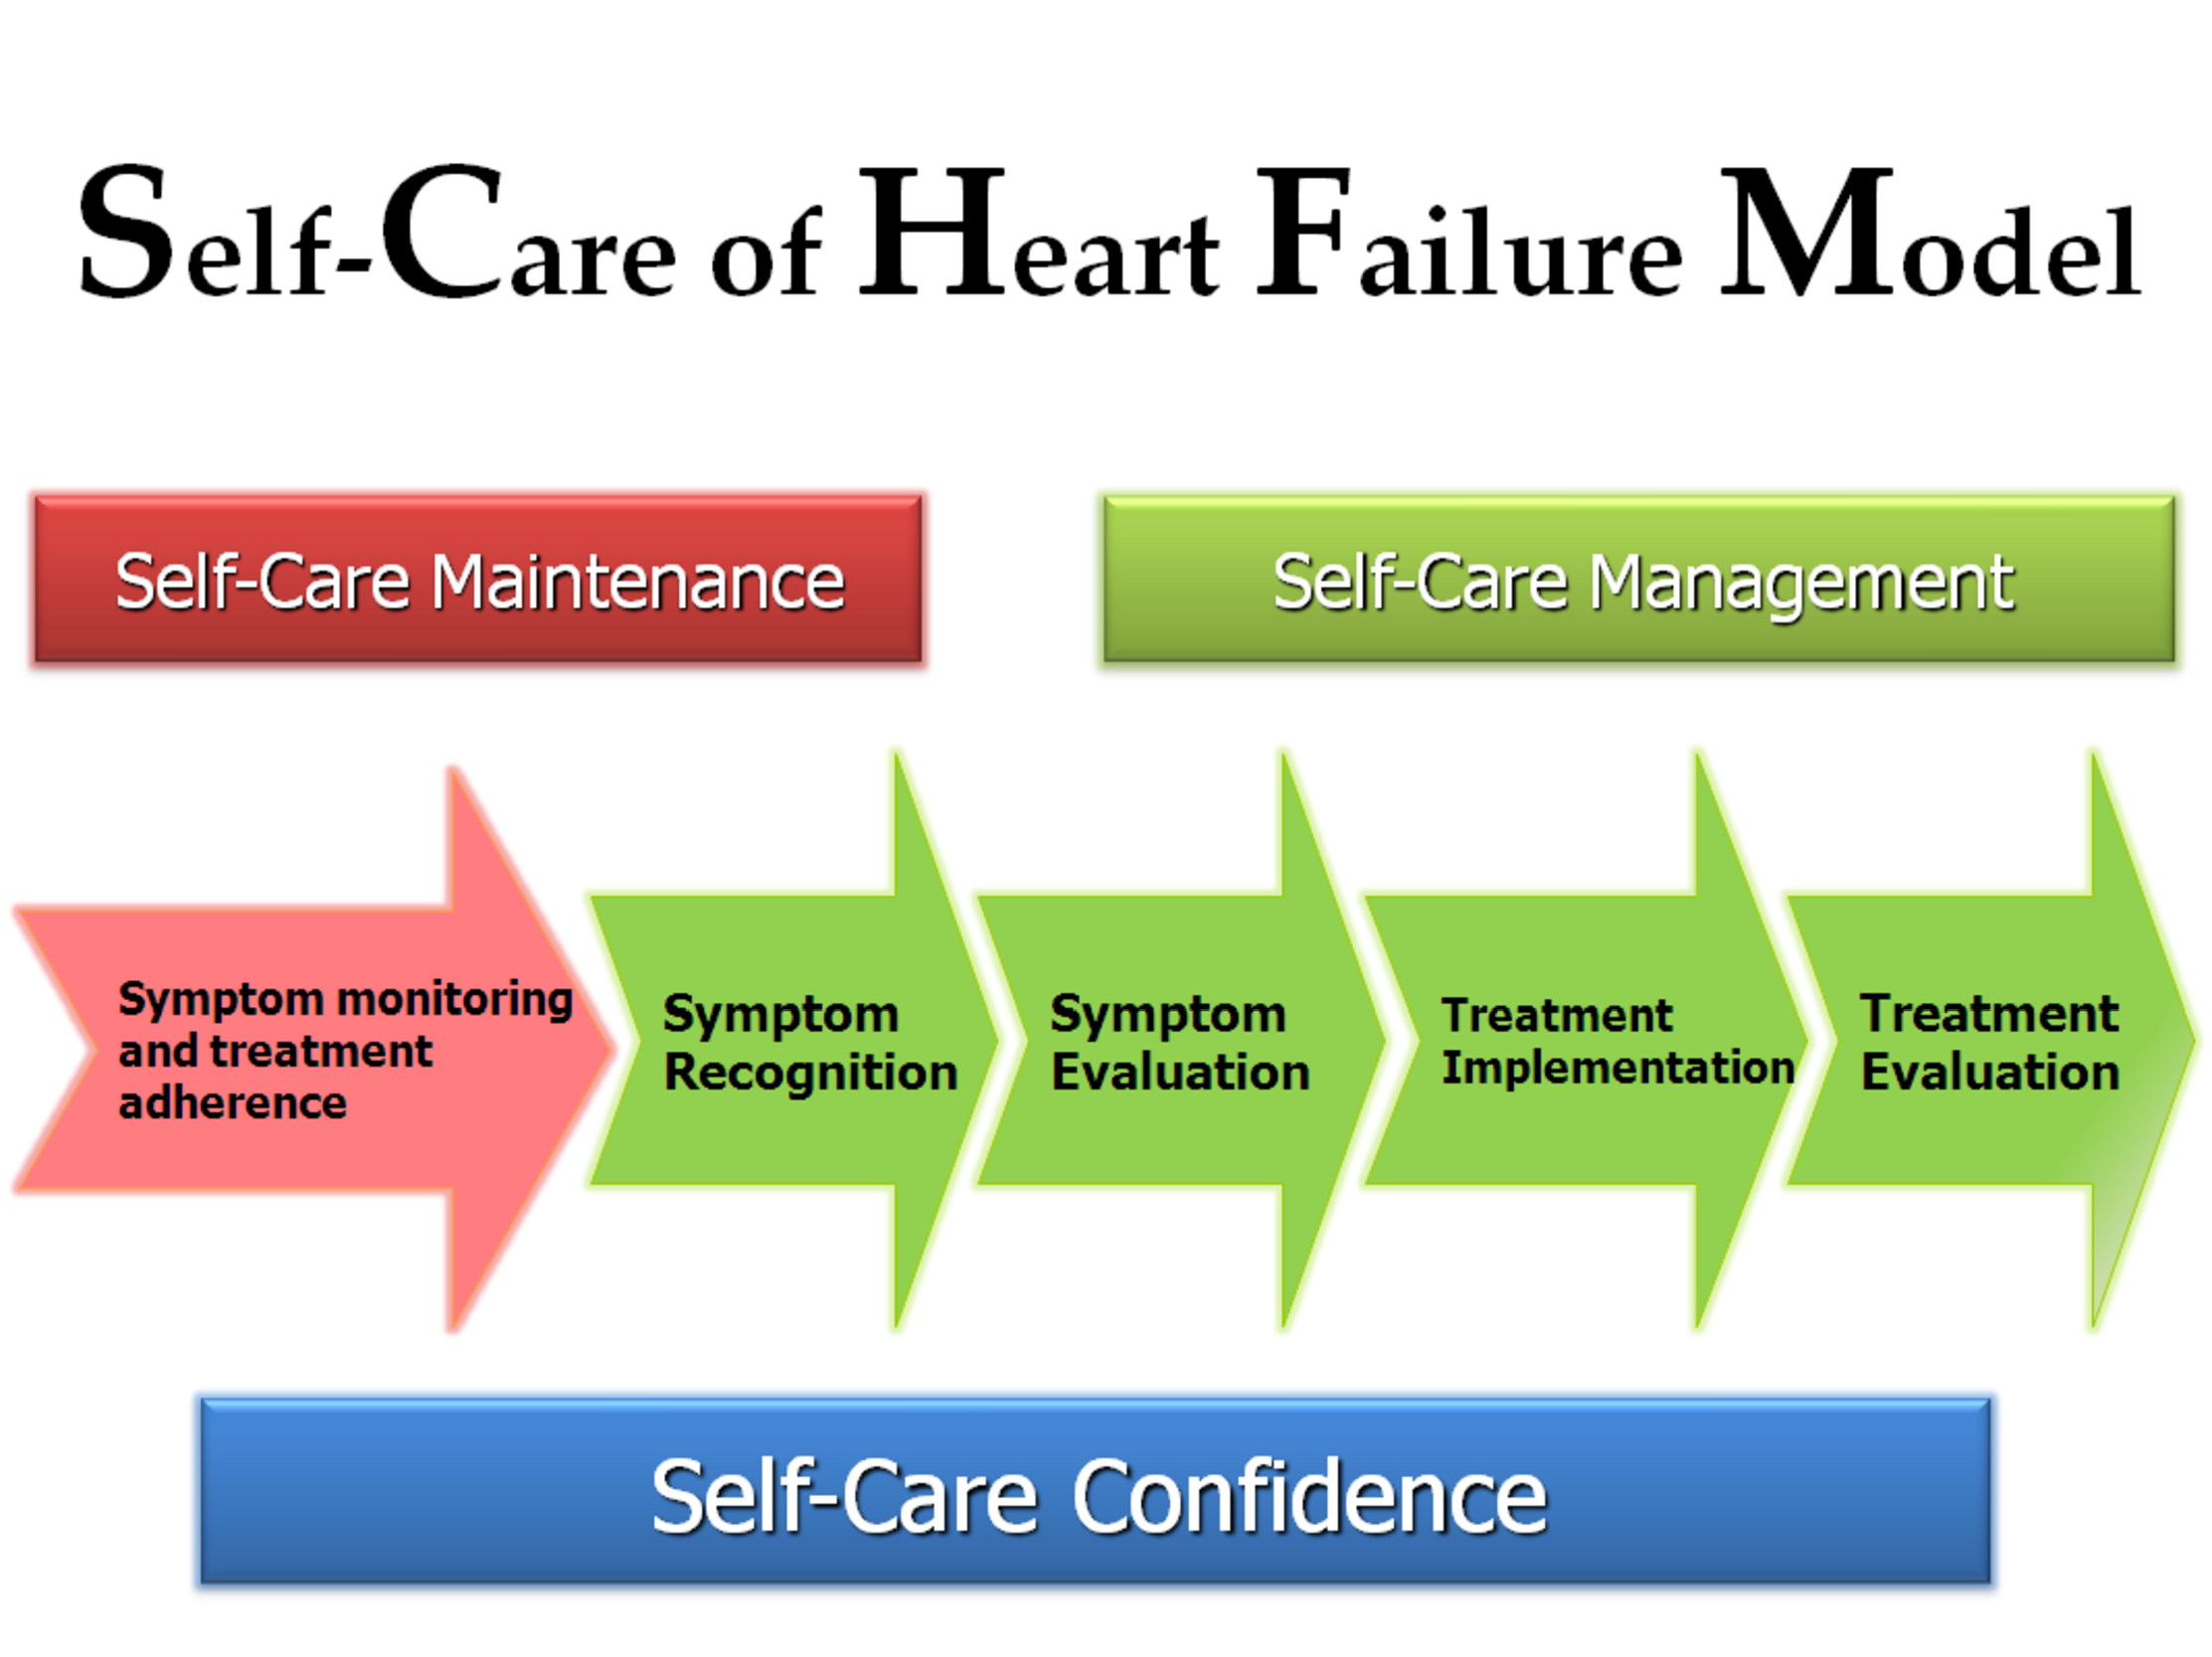
\includegraphics[scale=1,width=0.9\textwidth]{Images/SelfCare_cropped.pdf} 
		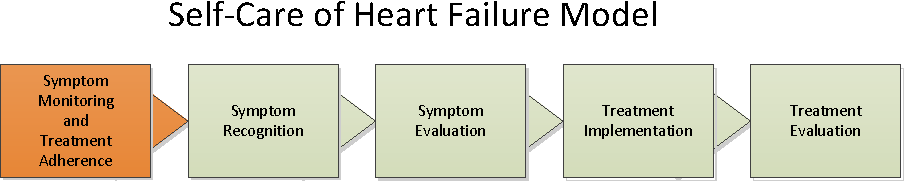
\includegraphics[scale=1,width=0.9\textwidth]{Images/SelfCare_recreated-cropped.pdf} 
		\caption{Theory of HF Self-Care }
		\label{fig:SelfCare}
	\end{center}
\end{figure}

With alerts to notify clinicians of an imminent event (an emergency) or a downward trend in need of correction, the WHIPPED system allows medical professionals to more effectively monitor a greater number of patients without degrading care. WHIPPED further provides a continuous link between patient and clinician which improves on the current visitation model, prescribed by Medicare, indicating that a home visit is needed after discharge and typically extends to ninety days post discharge \cite{Dansky2008}.

The dissertation will address the design, implementation, and testing of the WHIPPED Systems'  three parts: the WHIP sensor, the cellphone application, and the Back-end Knowledge Engine. The dissertation will also discuss the exploratory study, conducted by Dr. Sethares and its role in validating the WHIPPED System.

\section{Importance of Topic}
\label{sec:importanceOfTopic}

\begin{figure}
	\begin{center}

%		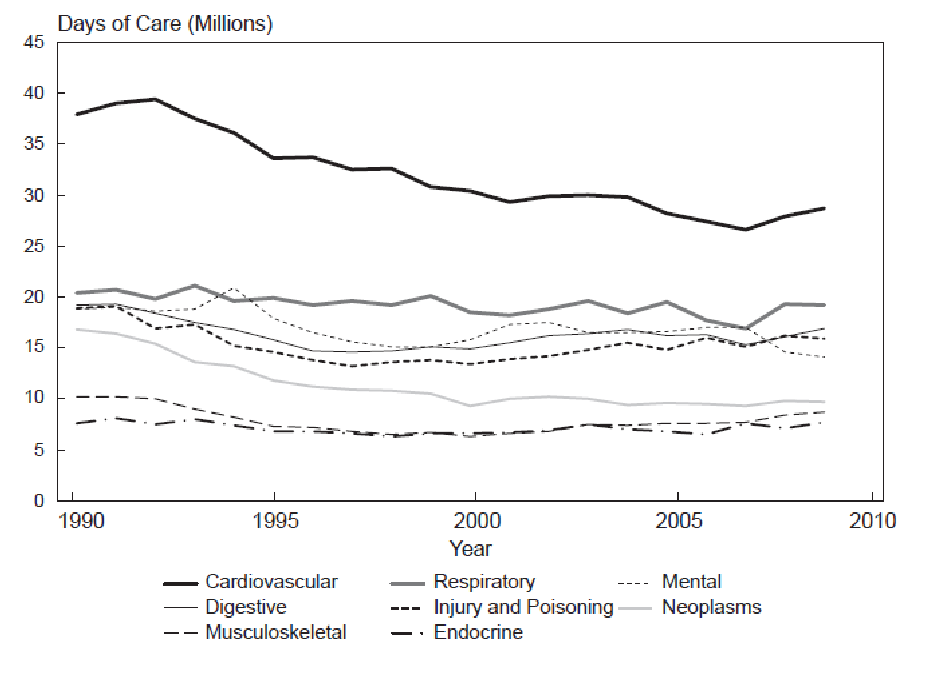
\includegraphics[scale=1,width=0.9\textwidth]{Images/DaysOfCare.png} 
		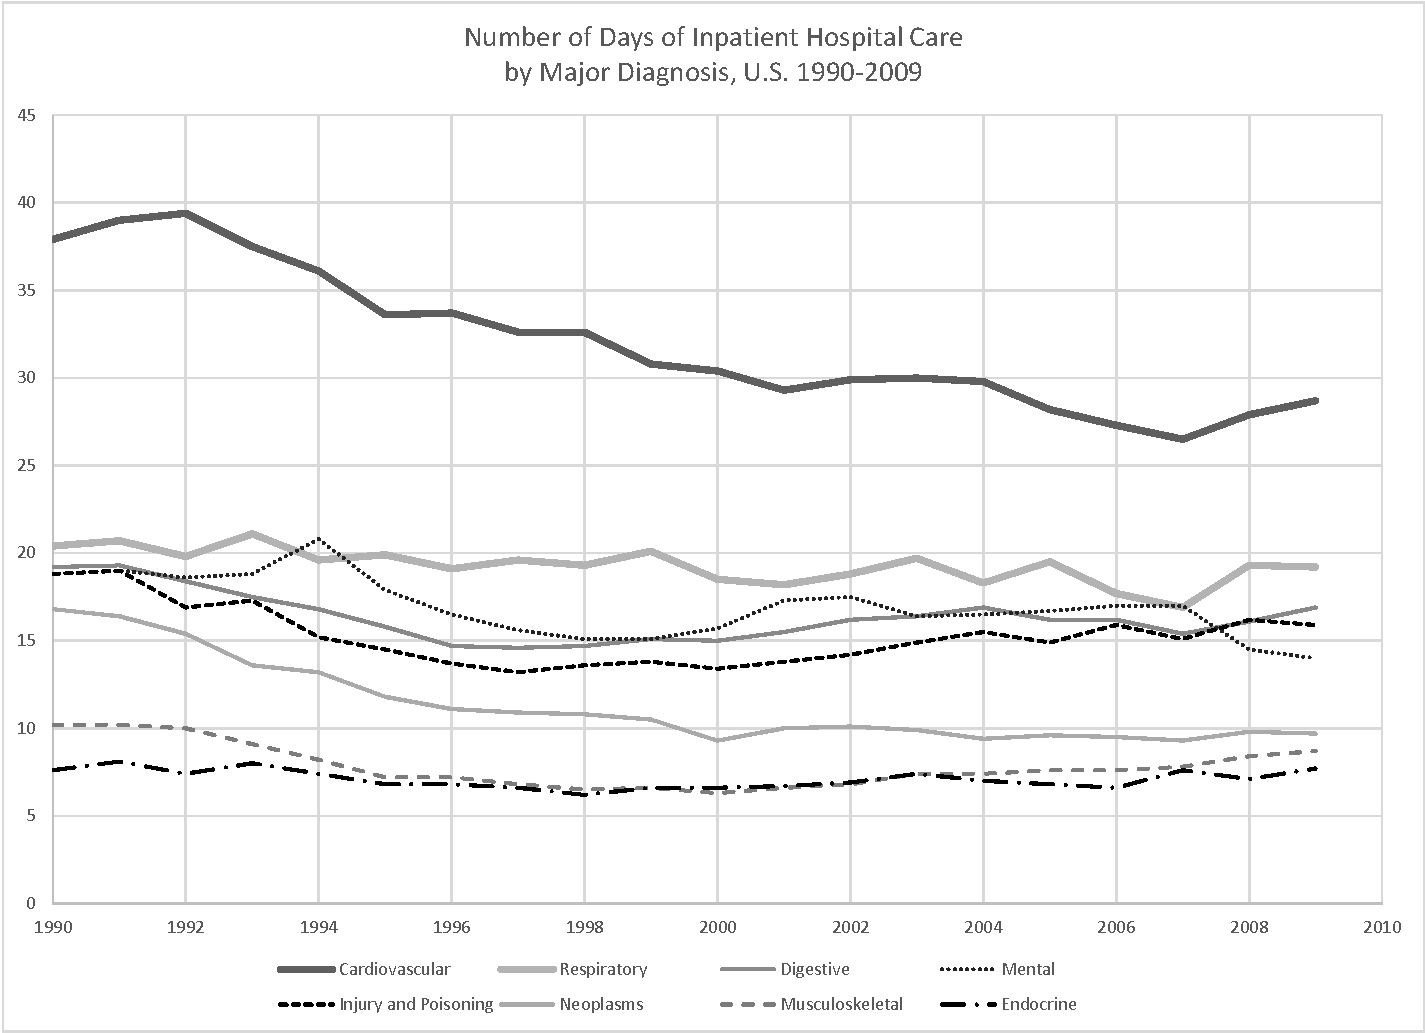
\includegraphics[scale=1,width=0.9\textwidth]{Images/CHD_cost_recreated-cropped.pdf} 
		\caption{Number of Days of Inpatient Hospital Care by Major Diagnosis U.S., 1990-2009 }
		\label{fig:DaysofCare}
	\end{center}
\end{figure}

Mussilino, working for the National Institutes of Health, compiled statistical data for the number of days of hospital care, required for different illnesses shown in  \cref{fig:DaysofCare} \cite{Mussolino2012}. Cardiovascular disease is clearly a major cost concern. Therefore, reducing re-hospitalization rates can substantially reduce the cost of cardiac care.


\begin{figure}
	\begin{center}
		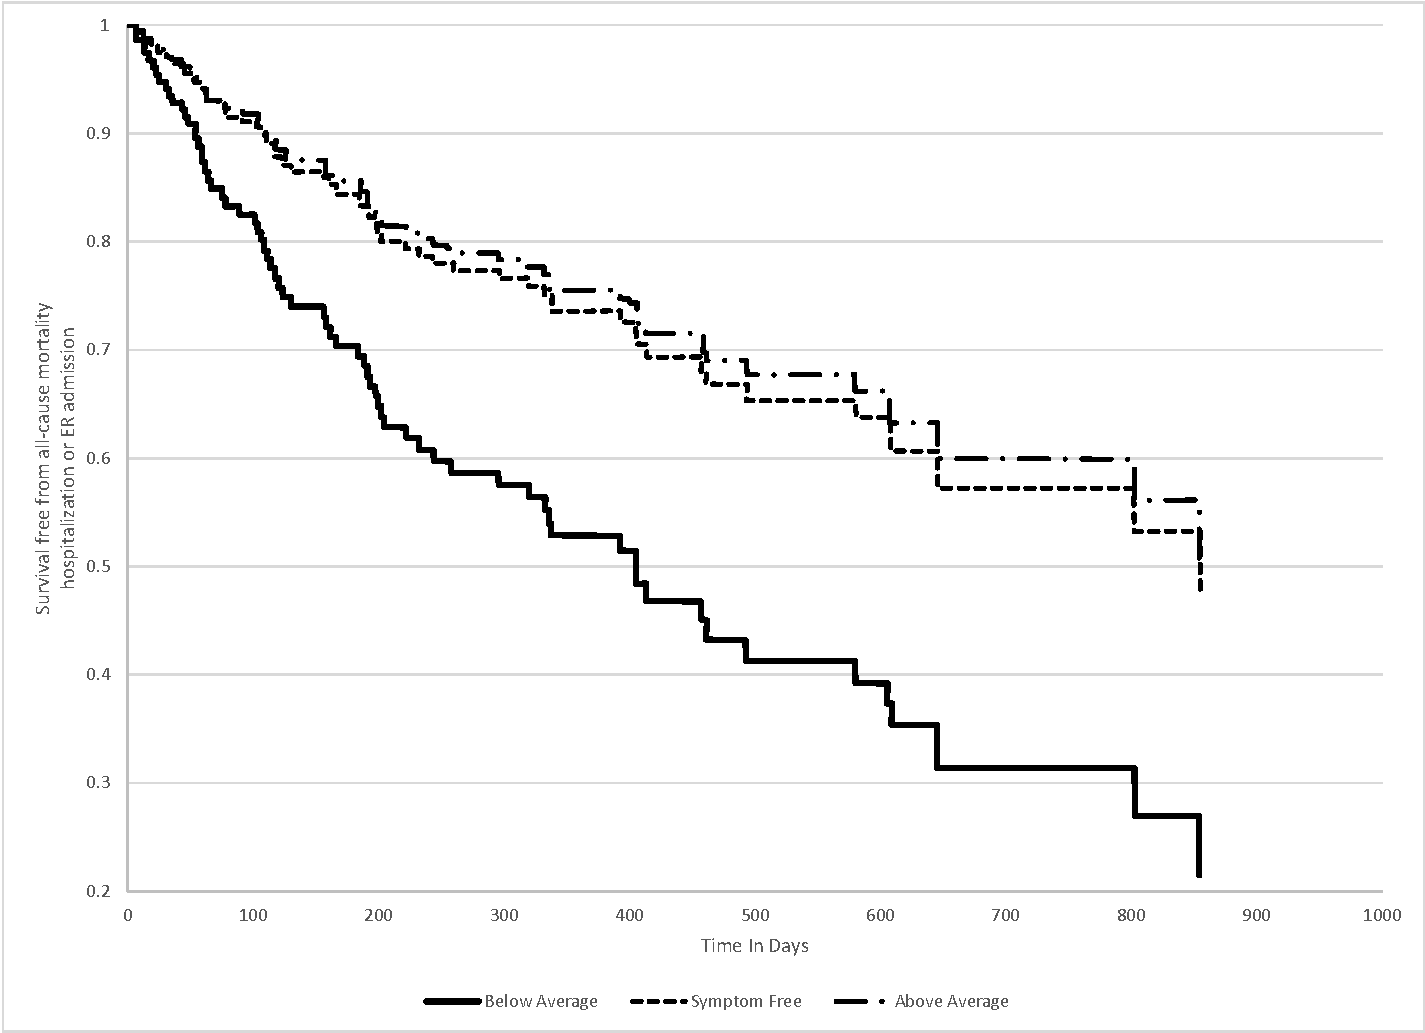
\includegraphics[scale=1,width=0.9\textwidth]{Images/daysOfCare_recreated-cropped (1).pdf} 
		\caption{Survival Rates of Patients who Engage in Self Care vs. Those That Do Not}
		\label{fig:SurvivalRates}
	\end{center}
\end{figure}


Lee et al. make a compelling case concerning patients who engage in self-care management \cref{fig:SurvivalRates}. \cite{Lee2011} The benefits of actively engaging patients in their own self-care can clearly be seen in their research.   Patients engaged in self-care management cut in half their risk of death, hospitalization, and need for emergency treatment compared to patient not involved in their own care. Furthermore, self-care managed patients with high-risk profiles were also shown to be nearly equivalent to patient who were symptom free \cite{Lee2011}.

Sethares and Elliott conduct a study providing tailored educational messages to patients to induce healthy self-care behaviors \cite{Sethares2004249}. Sethares and Elliot assess patient's QOL in their study using the Minnesota Living with Heart Failure questionnaire (MLHF). These tailored educational messages, from now on called interventions, were designed to encourage patients to engage in self-care such as taking medication on time, following a low sodium diet, etc. The statistical analysis showed patients were more likely to engage in self-care behaviors given these tailored message interventions. The study also did not show a significant decrease in re-hospitalizations. 


However, one of the limitations of Sethares and Elliott's study, the inability to monitor actual self-care behaviors, suggests an avenue for improvement, or augmentation of the tailored message interventions. Several other proven instruments for measuring perceived patient status exist including the Heart Failure Somatic Awareness (HFSA) \cite{Jurgens2006} test and the Duke Activity Status Index (DASI) \cite{Hlatky1989}. Using a combination of the MLHF, HFSA, and DASI instruments, self-care management can be augmented by allowing treatment evaluation \cref{fig:SelfCare}.   

According to Mussolino, Cardiovascular diseases were the leading cause of hospitalization for at least the past two decades. Moreover the cost of cardiovascular disease in 2008, as outlined in \cref{fig:CVDCost}, was \$297.7 billion \cite{Mussolino2012}. If patients are involved in their own self-care, and made aware of their state of wellness, so they can act on it and affect change, the financial strain on the health-care system can be greatly reduced. Some research to provide automated educational material to patients based on clinical practice guidelines (CPGs) showed promise \cite{Jones2005}. Further research, directed at producing protocols, based on best evidence practices, more accessible and editable by medical professionals emphasizes their need and value \cite{Shah2001}.

\begin{figure}
	\begin{center}
\begin{tabular}{lrrr}
          \null     & \multicolumn{3}{c}{Dollars (Billions)}                                                 \\ \cline{2-4}
Disease        & \multicolumn{1}{c}{Total} & \multicolumn{1}{c}{Direct} & \multicolumn{1}{c}{Mortality} \\ \hline

Total CVD      & 297.7                     & 179.3                      & 118.4                         \\
\hspace{4pt} Heart disease  & 190.3                     & 95.6                       & 94.7                          \\
\hspace{4pt} Stroke         & 34.3                      & 18.8                       & 15.5                          \\
\hspace{4pt} Hypertension   & 50.6                      & 47.4                       & 3.2                           \\
\hspace{4pt} Other CVD      & 22.5                      & 17.5                       & 5.0                           \\
Hyperlipidemia & 39.8                      & 38.6                       & 1.2                           \\
COPD/asthma    & 68.0                      & 53.7                       & 14.3                          \\
Pneumonia      & 20.4                      & 14.0                       & 6.4                           \\
Anemias        & 5.9                       & 4.7                        & 1.2                           \\
               &                           &                            &                              
\end{tabular}

		\caption{Economic Cost of Cardiovascular, Lung, and Blood Diseases U.S., 2008 }
		\label{fig:CVDCost}
	\end{center}
\end{figure}

\section{Problem Statement}
\label{sec:problemStatement}
The evidence presented, indicates a need for the WHIPPED system. WHIPPED collects both the psychosocial data from instruments like the HFSA, DASI, and MLHF and biometric data from the wireless sensor suite.  WHIPPED correlates the collected data to provide more timely feedback to a patient in the first days, weeks and months of their discharge from the hospital after a HF related event as needed. WHIPPED must have as little physical impact on a user as possible. WHIPPED utilizes non-invasive synthetic sensor technologies to derive common cardiac metrics using a minimal number of physical measurements. 

Currently, disparate research exists to collect cardiac metrics with an acceptable level of accuracy given only one or two transducers. The goal of the dissertation is the design, implementation, and testing/validation of the complete end-to-end WHIPPED system. Key features of the system are:

\begin{itemize}
\item The use of synthetic sensor measurements to detect cardiac metrics, specifically ECG, \spo2, blood pressure, respiration, and heart rate.
\item A hardware, firmware, and software implantation of a cardiac sensor suite.
\item The development of a wellness measure, to classify and indicate patient's cardiac heath and overall wellness. \cite{Chaiyasucheeva2012}
\item The ability to offer interventions to engage a patient in self-care.
\item Remote monitoring capabilities for clinicians, offering direct interaction with patients.
\end{itemize}

In addition, the dissertation develops techniques for fusing the collected information, consulting with a CPG or specialized cardiac ontology and providing cardiac-wellness feedback to engage a patient in their self-care regimen. Using feedback and motivated self-interventions patients can follow up on their conditions with more rigor than currently possible given current institutional and personnel limitations, possibly at a greatly reduced cost. Additionally, a system is proposed whereby medical professionals can monitor patient's wellness, to offer additional interventions as needed.

\section{Hypothesis}
\label{sec:Hypothesis} 
In the dissertation research, we are designing, developing, and testing an end-to-end system, along with proposing an exploratory study using a mix of technologies, proven evidence based practices, interventions to aid patients in learning about and becoming involved in home self-care. During the dissertation's research, we will determine if technology can assist patients to understand their own illness, and act to improve their QOL and decrease the chance of re-hospitalization. 

Subsequently, when designing and experimenting with the WHIPPED system we propose to answer several questions. First, will patients use the technology? Second, will the technology aid patients in understanding their disease?  Third, can patients learn to act in improving their overall wellness? When considering adoption of the technology we propose looking at the smartphone by itself, the smartphone and sensor suite, the sensors themselves and a control group. If patients fully adopt the system, both the smartphone for its psychosocial elements and the sensors for the physiologic data, most robust analysis can be performed. Full technology adoption may allow us to answer, possibly, another question; is there a correlation between perceived wellness, as reported using the psychosocial data, and actual wellness, derived through sensor measurements? If the patient only uses the smartphone, no physiologic data can be gathered and only the perceived status of the patient can be discerned. Similarly, if the patient does not complete any of the psychosocial questionnaires only the biometric readings will be available. The dissertation hypothesizes we can improve patient QOL, reduce the need for re-hospitalization, and therefore lower costs by implementing the proposed system, primarily by educating the patient, using evidence based best practice philosophies.


\section{Research Approach}

In order to actualize the WHIPPED system the design is divided into three parts: the sensor suite, the smartphone application, and the BKE. Each piece will be designed and the interfaces between each part specified. Before designing can take place however, the responsibilities of the system must be divided and the requirements of the system must be applied to each part of the system.

The sensor suite is envisioned as a wearable patch, requiring no advanced medical knowledge to apply. Furthermore, since it is the main physical part of the system, and the goal of the system is to be low cost, the sensor suite must be as low cost as possible. The device will implement sensors to collect real-time ECG and \spo2 measurements to satisfy these requirements. The system will be responsible for deriving all other physiological measurements. The sensor suite should be small, battery powered, and capable of wireless communication with the smartphone. 

The smartphone will perform three main functions. First, it will receive and retransmit the biometric data to BKE, capable of mining the received data. Second, the smartphone will periodically assess the patient using psychosocial instruments, such as the DASI and HFSA, further augmenting the data received from the sensors. The third, and final, task of the smartphone is to receive data from the BKE. The BKE can deliver a calculated wellness measure, auto generated tailored interventions, medical reminders (e.g. take medication), or messages from the clinician. We seek to validate good behavior on the part of the patient and discourage unhealthy behavior by providing the wellness measure to the patient. 

Auto-generated interventions will not provide suggestions requiring a clinician, such as a prescription, but will instead be changes to the CHF patient's lifestyle, such as diet or exercise, to increase the wellbeing and the longevity of the patient while decreasing the risk of re-hospitalization. 

Patients will be able to view their wellness, ECG, \spo2, respiration, and heart rate history as temporal graphs. Temporal graphs will aid patient's learning about how their activity (e.g. adherence to interventions, taking medications) affects their overall wellbeing.

The BKE will make use of a minimal cardiac ontology with co-morbidity information to assess a patient's status. The wellness metric will be based on the collected biometric readings as well as the psychosocial instruments correlated with the medical ontology to calculate the patient's overall wellness. We will also track the patient's wellness over time, and, if a decreasing trend is detected in the patient's wellness score, provide possible interventions to the user to reverse the downward trend. Finally, in severe cases we can provide an alert to a medical professional indicating immediate care is needed.

Having defined the requirements and operation of the system, focus can now switch to realization. The natural first choice is to construct a sensor platform to collect ECG and PPG readings. The ``\nameref{sec:ResearchDoneToDate}'' section shows significant progress in data collection has been achieved. While building the sensor suite, work also began on several smartphone applications. Early applications were responsible for displaying collected data in real time in order to validate the sensor designs. Work can begin on the design of the BKE, after sensor suite validation. The BKE is partitioned into four design tasks. 
\begin{itemize}
\item First a minimal EHR was designed and implemented. Identification of co-morbidities and demographic data storage are the primary goals of the initial EHR.
\item The second task will be to expand the EHR to support real-time biometric data and periodic psychosocial data. 
\item The third task is to design and implement a minimal cardiac ontology.
\item Lastly, the algorithms for wellness calculation and interventions can be implemented using data provide for the first three parts.
\end{itemize}
These four tasks will not be completed atomically. Part of building and validating a database is providing test data. The other parts of the system, the smartphone and WHIP, can be integrated with each BKE task. A smartphone app allowing “registration” can be written, after designing a minimal EHR , with the intention of integration into the final smartphone application. Once the EHR is expanded to support the sensor and psychosocial data, integrating the three parts of the system together can begin. Firmware for the sensor can be written, designed to transfer the data to the smartphone.  The smartphone will have a service to relay the sensor data to the BKE. The smartphone will also be able to administer psychosocial instruments. 
A secondary smartphone application can be written, geared towards a clinicians use, to monitor the data coming from the sensor suite. Once the data transfer to the BKE is tested and verified the task of wellness calculation and intervention analysis can begin. Validation of the back-end computations is accomplished using simulated patient data input into the database. Patient simulations will seek to test the wellness calculations validity. The smartphone app will be augmented to receive data from the BKE and deliver the wellness calculation to the patient simulation. The BKE will also be presented with simulated patients who have decreasing wellness scores and will be tested to see what types of interventions are provided. The emergency feature of the system can be implemented and tested without the BKE; designed to call an urgent care center if a cardiac event, such as a heart attack, is detected. If the sensor suite detects such an event, it should send an alert to the smartphone. The phone can then place a call and automatically deliver information such as location, type of event detected, and patient information to the operator. The phone can then connect the operator to the patient if they are conscious, to allow further information to be communicated. During testing of the emergency response feature another number can be substituted for 911. Then a simulated event can be input into the system to test if the event is detected and the phone call placed. Once the functionality of these devices has been verified, an exploratory research study is proposed to validate the system with real world participants.

\section{Limitations and Key Assumptions}
\label{sec:LimitationsAndKeyAssumptions}
The WHIPPED system could be expanded to many domains. However, we bound the research in several areas. When we move to real world patients, we will seek between ten and twenty participants for an experimental study, not a clinical trial. A study allows us to select patients who will most benefit from the system, specifically patients over sixty-five who have had one or more cardiac events. We are further limiting ourselves in the area of design to consider non-invasive methods of data collection. While there have been long-term implantable devices developed [54], these are not suitable for the dissertation's purposes. Creating a system having the smallest possible impact on the day-to-day activities of the patient is significant goal of the research. Therefore, any device which connects to a patient, must be in a small form factor. If the device is to be removable, it must not require any special knowledge to re-affix the device.  Furthermore, the device should be designed with long-term use in mind. Since the device must be portable, battery power is needed. Battery power further implies the device must be low power.

\section{Contributions to Knowledge}
\label{sec:ContributionsToKnowledge}
Due to the interdisciplinary nature of this dissertation, contributions can be split into two areas: the contributions to the medical domain and the contributions to the engineering domain. The medical domain can benefit by using the WHIPPED system to test the hypothesis that engaging patients in their own self-care can lead to a better QOL and reduce hospitalization. During the exploratory study, tests will be performed based on patients who use the traditional care method (the control), patients using only the psychosocial instruments, and patients who have the sensors and psychosocial instruments. We can also access if patients will effectively use the system to facilitate their self-care.
For the engineering domain, we will develop new and novel techniques for data fusion and knowledge acquisition supporting numerous future applications (e.g. future soldier systems, athlete training). We will design implement and validate an end-to-end system that integrates synthetic sensors, wireless communication, and the calculation of a wellness measure, using an EHR and BKE into an all-inclusive system. We will provide a medical solution to engage patients in their own self-care cheaply with little impact on the user. The WHIPPED solution can reduce health-care costs and increase QOL. 

\section{Research Done to Date}
\label{sec:ResearchDoneToDate}
In preparation for the main research component of the dissertation, some preliminary work in the fields of bio-sensing has already been performed . The first step was to get up to speed on the research group's status. During the 2009-2010 school years, a senior design group was tasked with building an analog front end to capture an ECG signal. Also, during the 2009-2010 school years, master's candidate Osama Aljaroudi designed an analog front-end excitation and conditioning circuit for a \spo2/PPG circuit. A device with both circuits was designed and fabricated on a four-layer PCB board and shown in \cref{fig:PCB_alpha}. Unfortunately, because of the inexperience with the tools the board suffered from many problems. These were eventually rectified with “green wire fixes”. A great deal was learned from the initial foray into fabrication.

\begin{figure}
	\begin{center}
		
		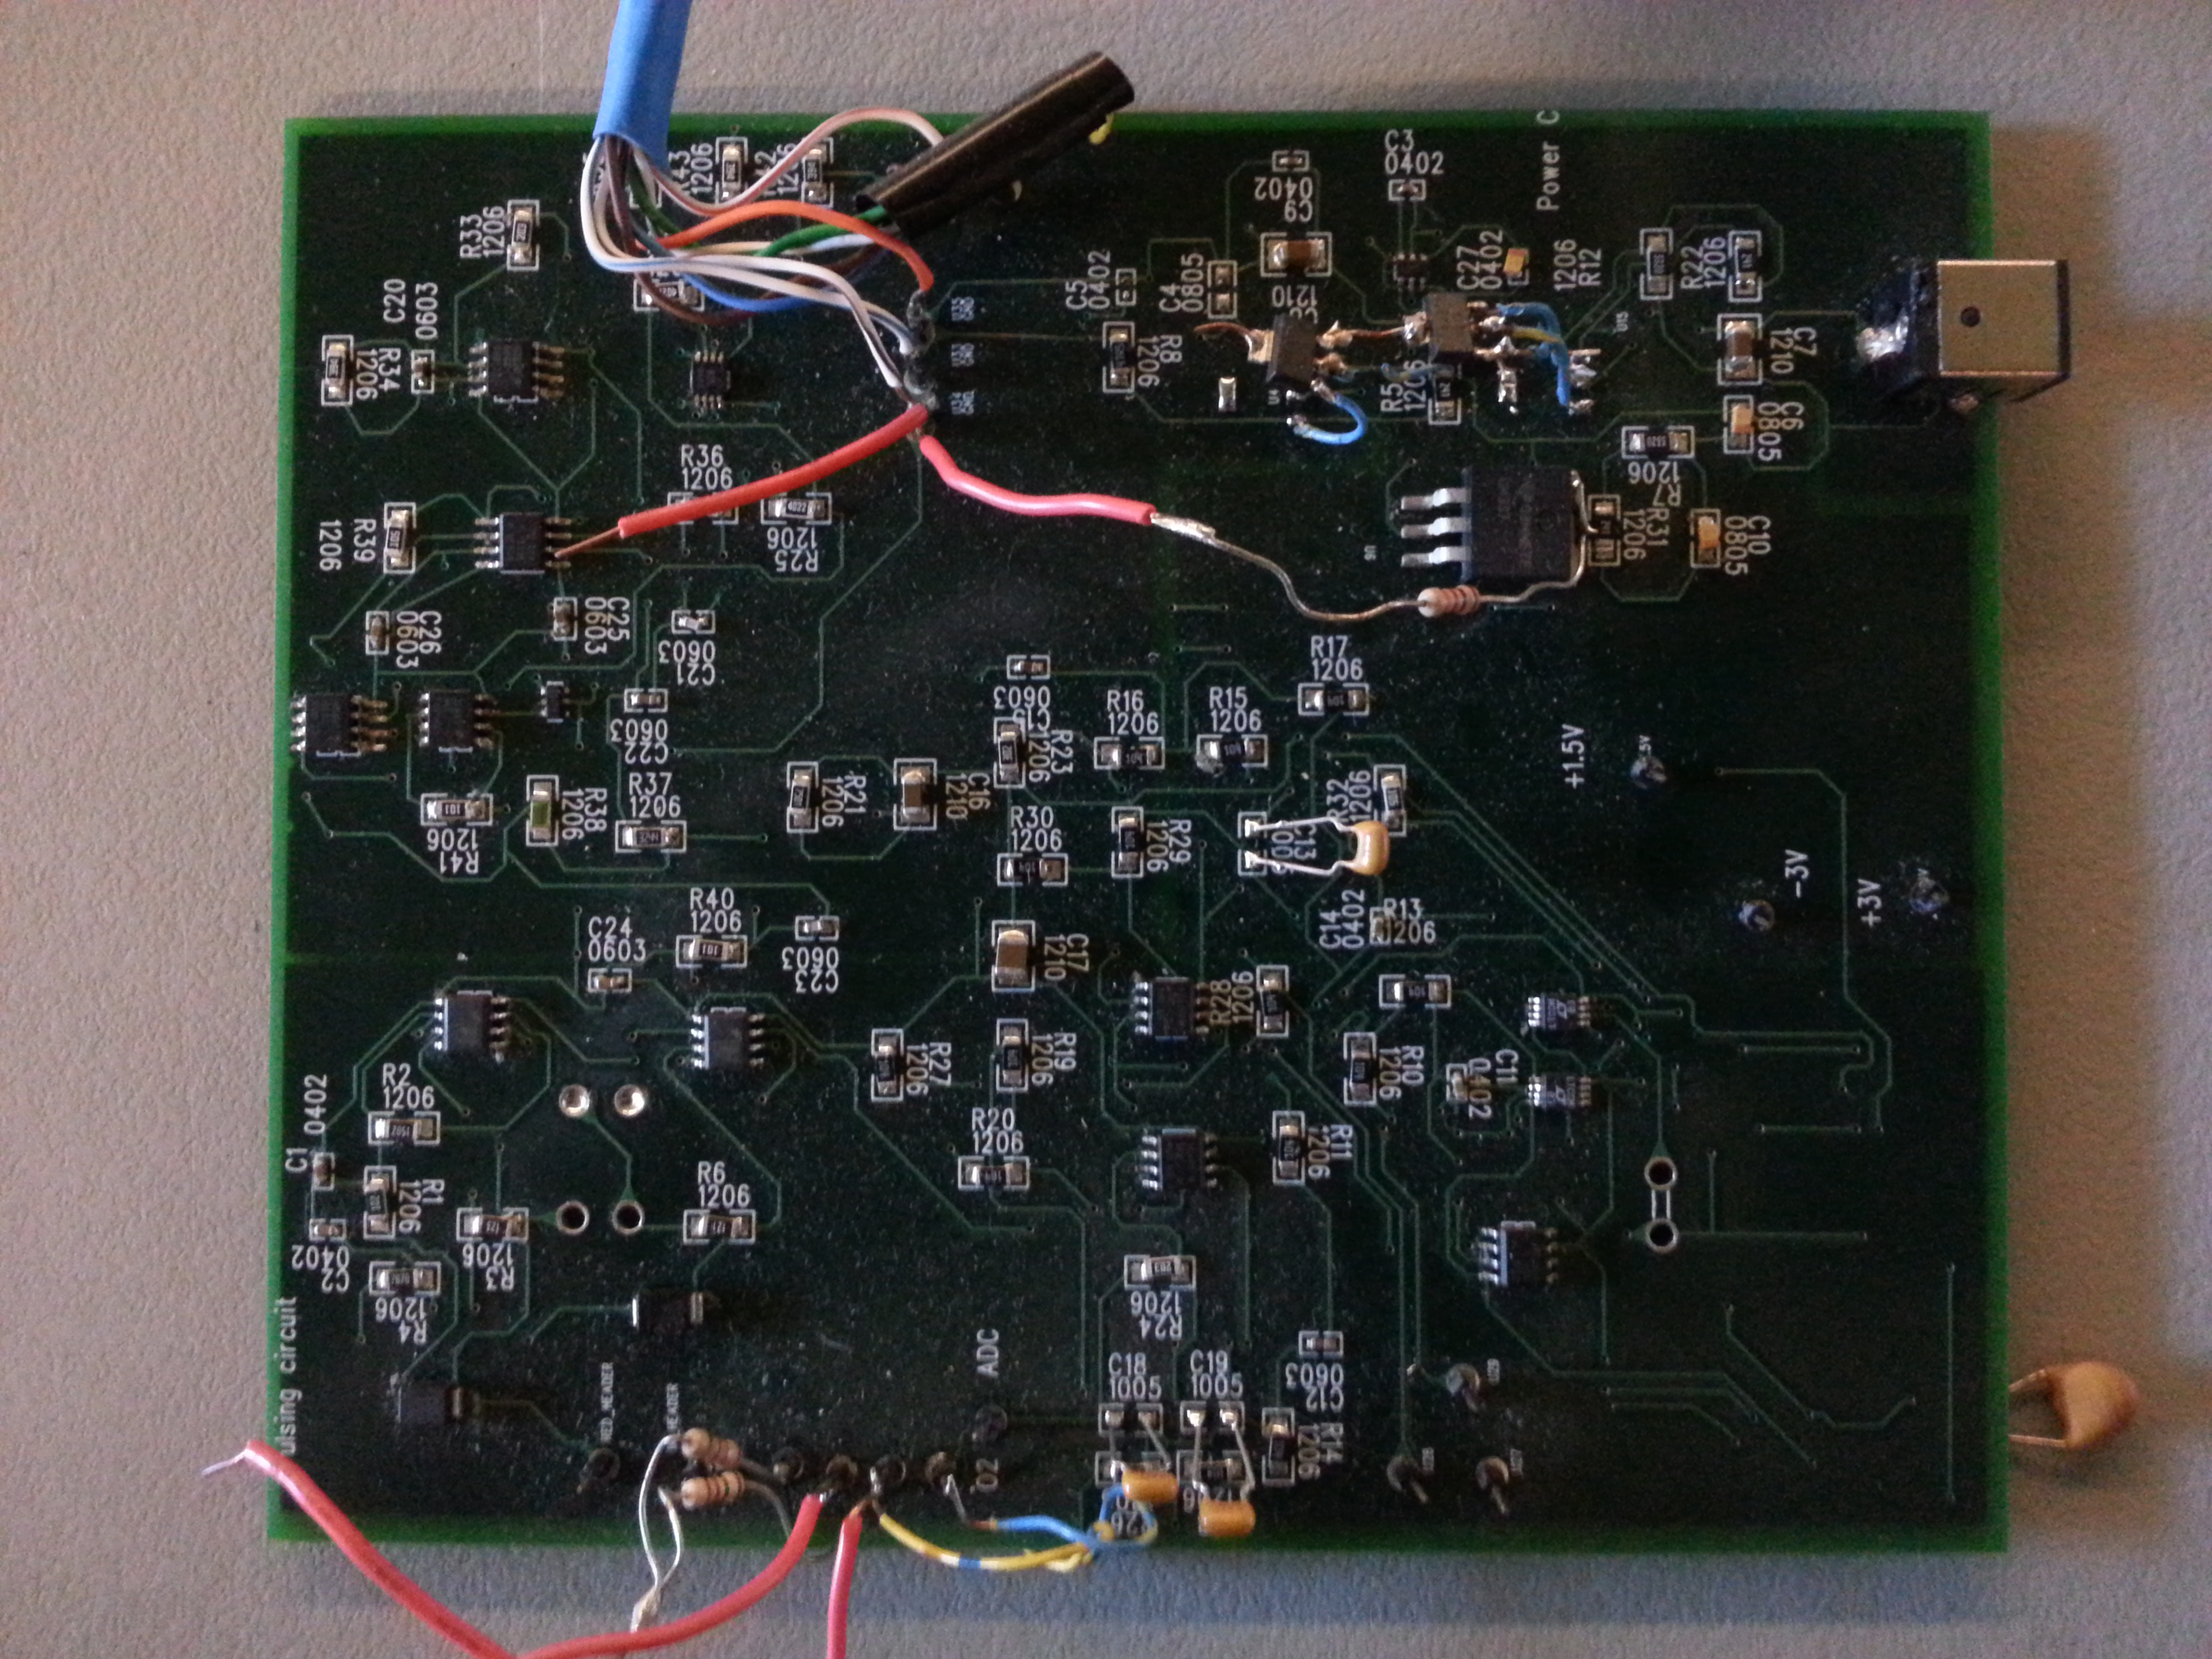
\includegraphics[scale=1,width=0.9\textwidth]{Images/PCB_Alpha.jpg} 
		\caption{Analog Front-end Alpha Board.}
		\label{fig:PCB_alpha}
	\end{center}
\end{figure}

The next revision of the hardware was personally undertaken by me in the spring of 2011. Referred to as Revision Alpha, the design miniaturized the footprint of the analog front end. The design utilized an adaptation of the senior design group's ECG circuit and the master candidate's \spo2 circuit. Alpha's design utilized surface mount integrated circuits (ICs) and through-hole passive components. The prototype sensors were fabricated as a two-layer board shown in \cref{fig:PCB_analog_beta}. Some calculated resistances needed to be fabricated by soldering some components to each other “dead-bug” style due to lack of available stock. The lesson learned: check what parts are available before finalizing a design.

\begin{figure}
	\begin{center}
		
		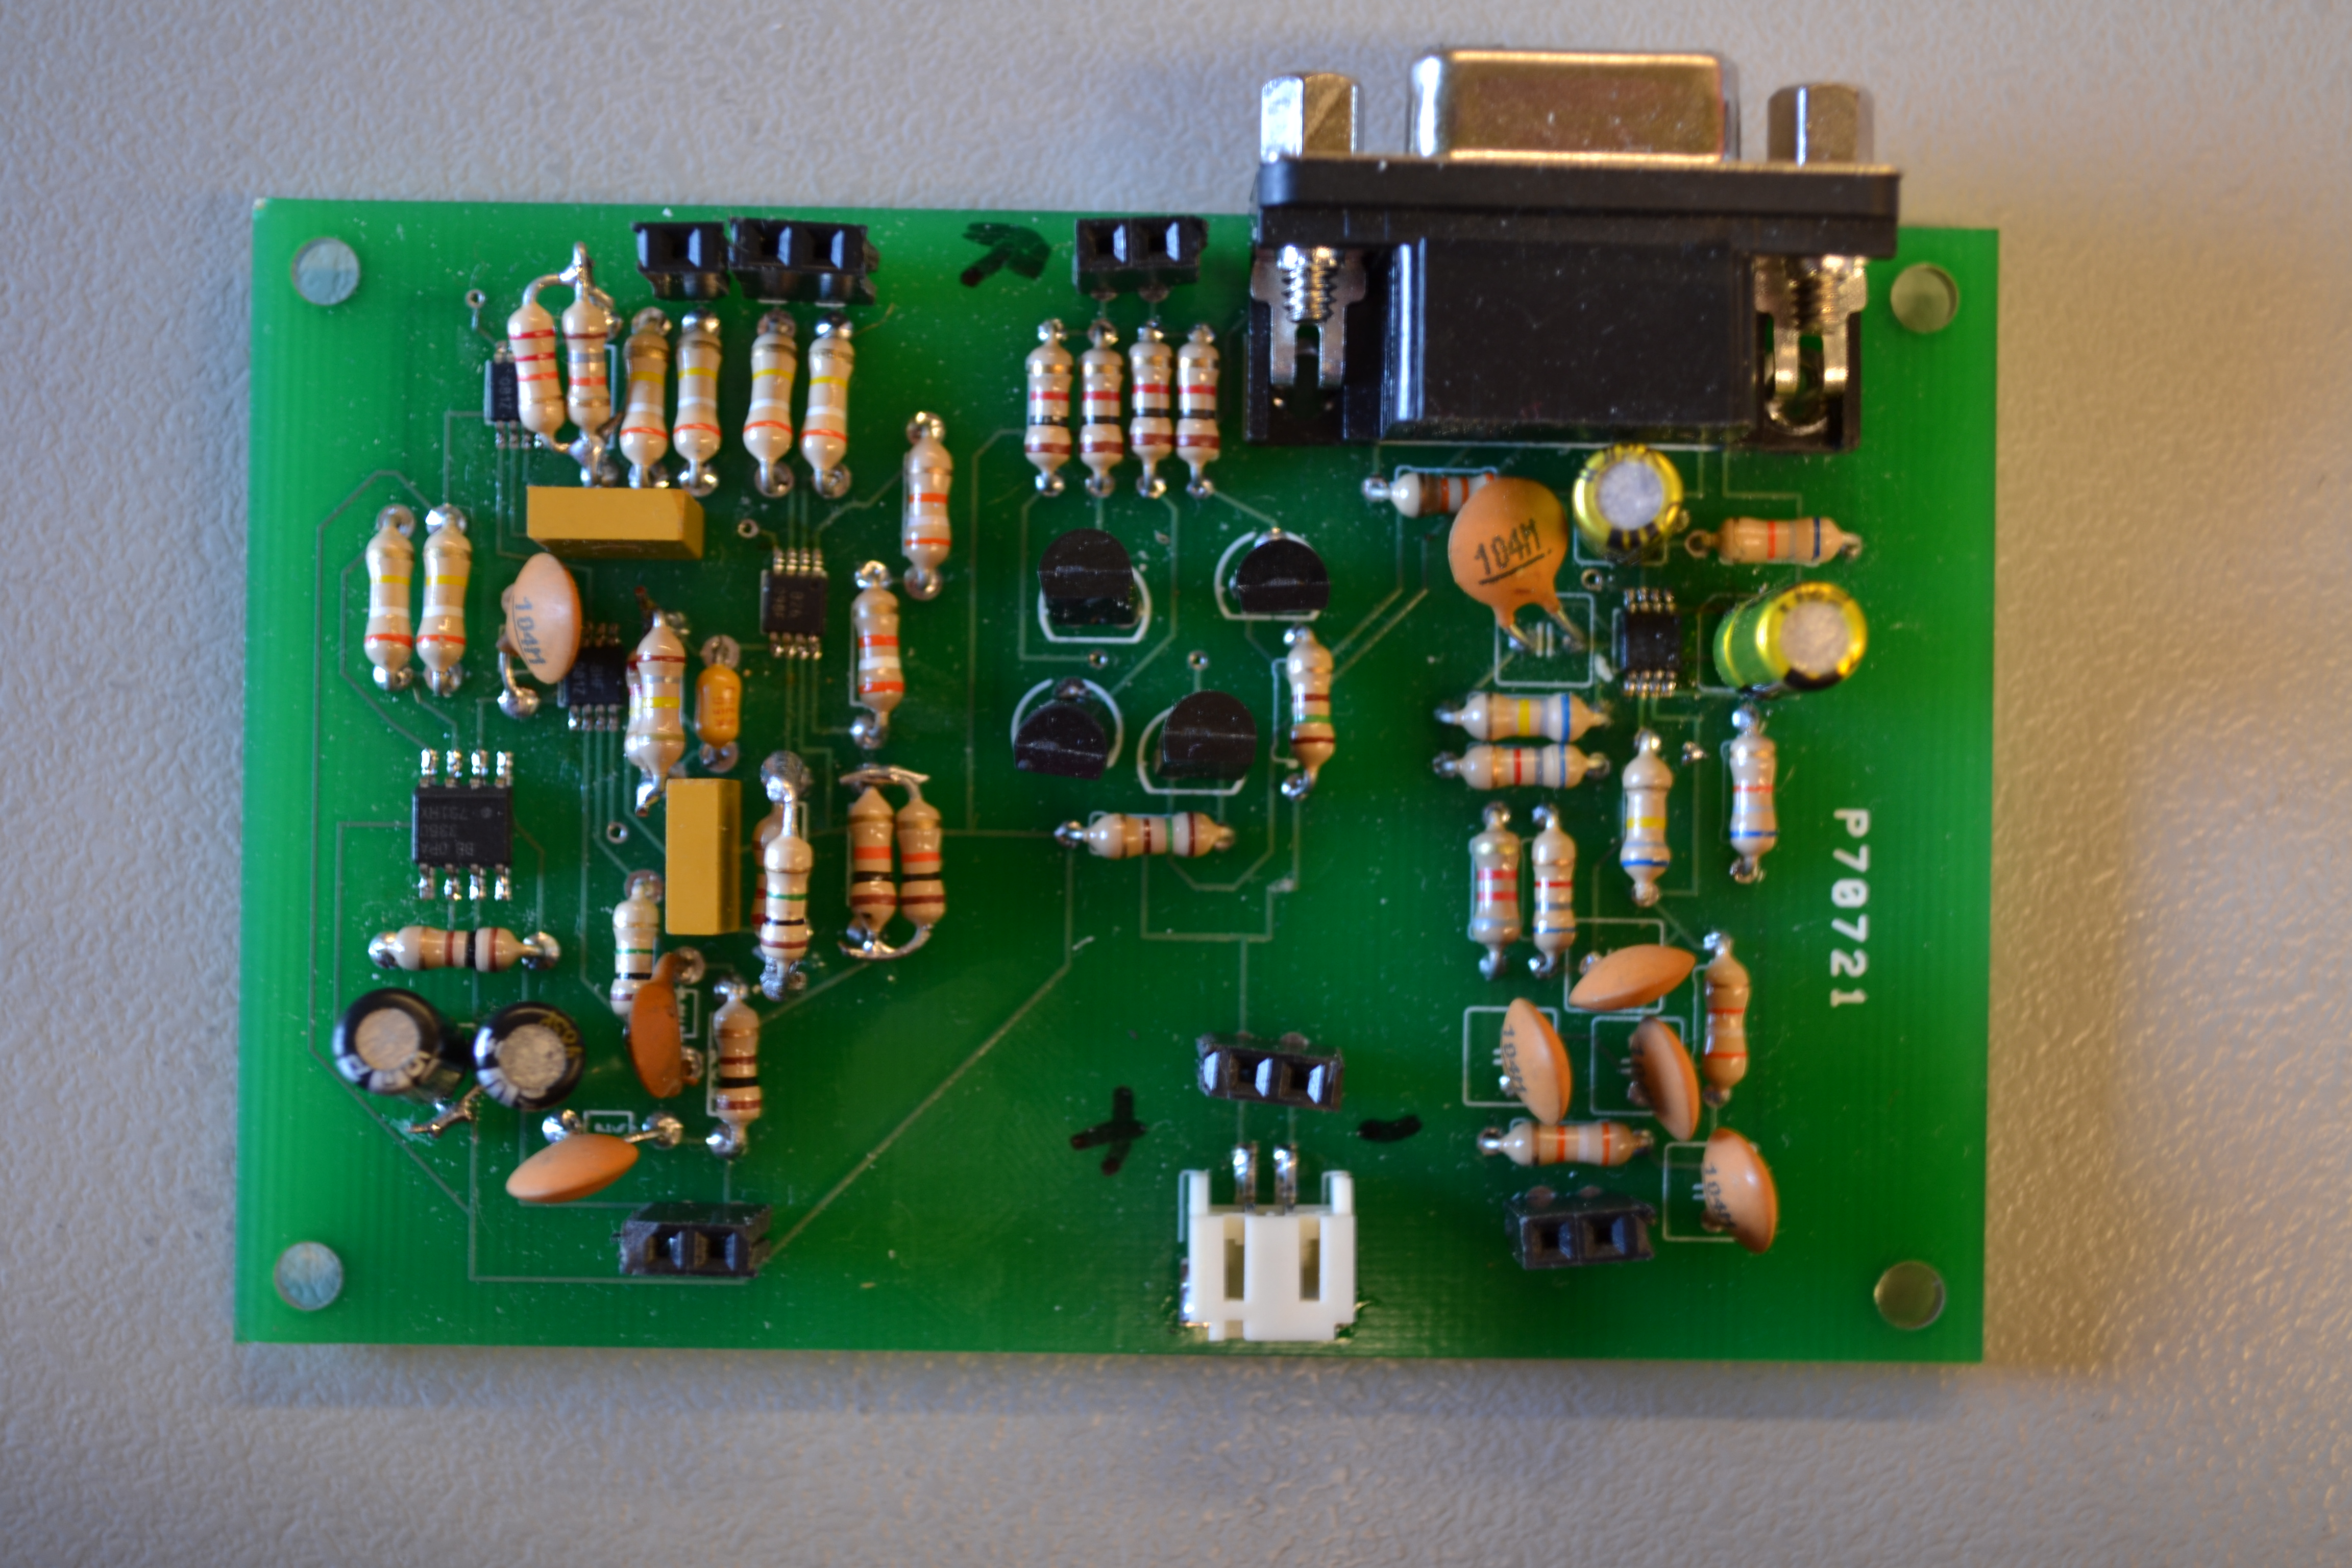
\includegraphics[scale=1,width=0.9\textwidth]{Images/PCB_AnalogBeta.JPG} 
		\caption{Beta Analog Board}
		\label{fig:PCB_analog_beta}
	\end{center}
\end{figure}

To interact with the analog front-end board a controller PCB was manufactured in-house to host an ADuC7020 development socket. This board was designed in the same fashion, using the same tools as the analog front-end board but was manufactured by hand using an acid etching process and drilled on a CNC router (designed to improve the turnaround time and cost of prototypes). Front and back views are shown in \cref{fig:PCB_digital_beta}. The controller board served to validate the results of the initial analog designs. Using results from early prototyping work began on the first revision of an integrated solution. This board integrated as many components as possible into the sensor design.

\begin{figure}
	\begin{center}

		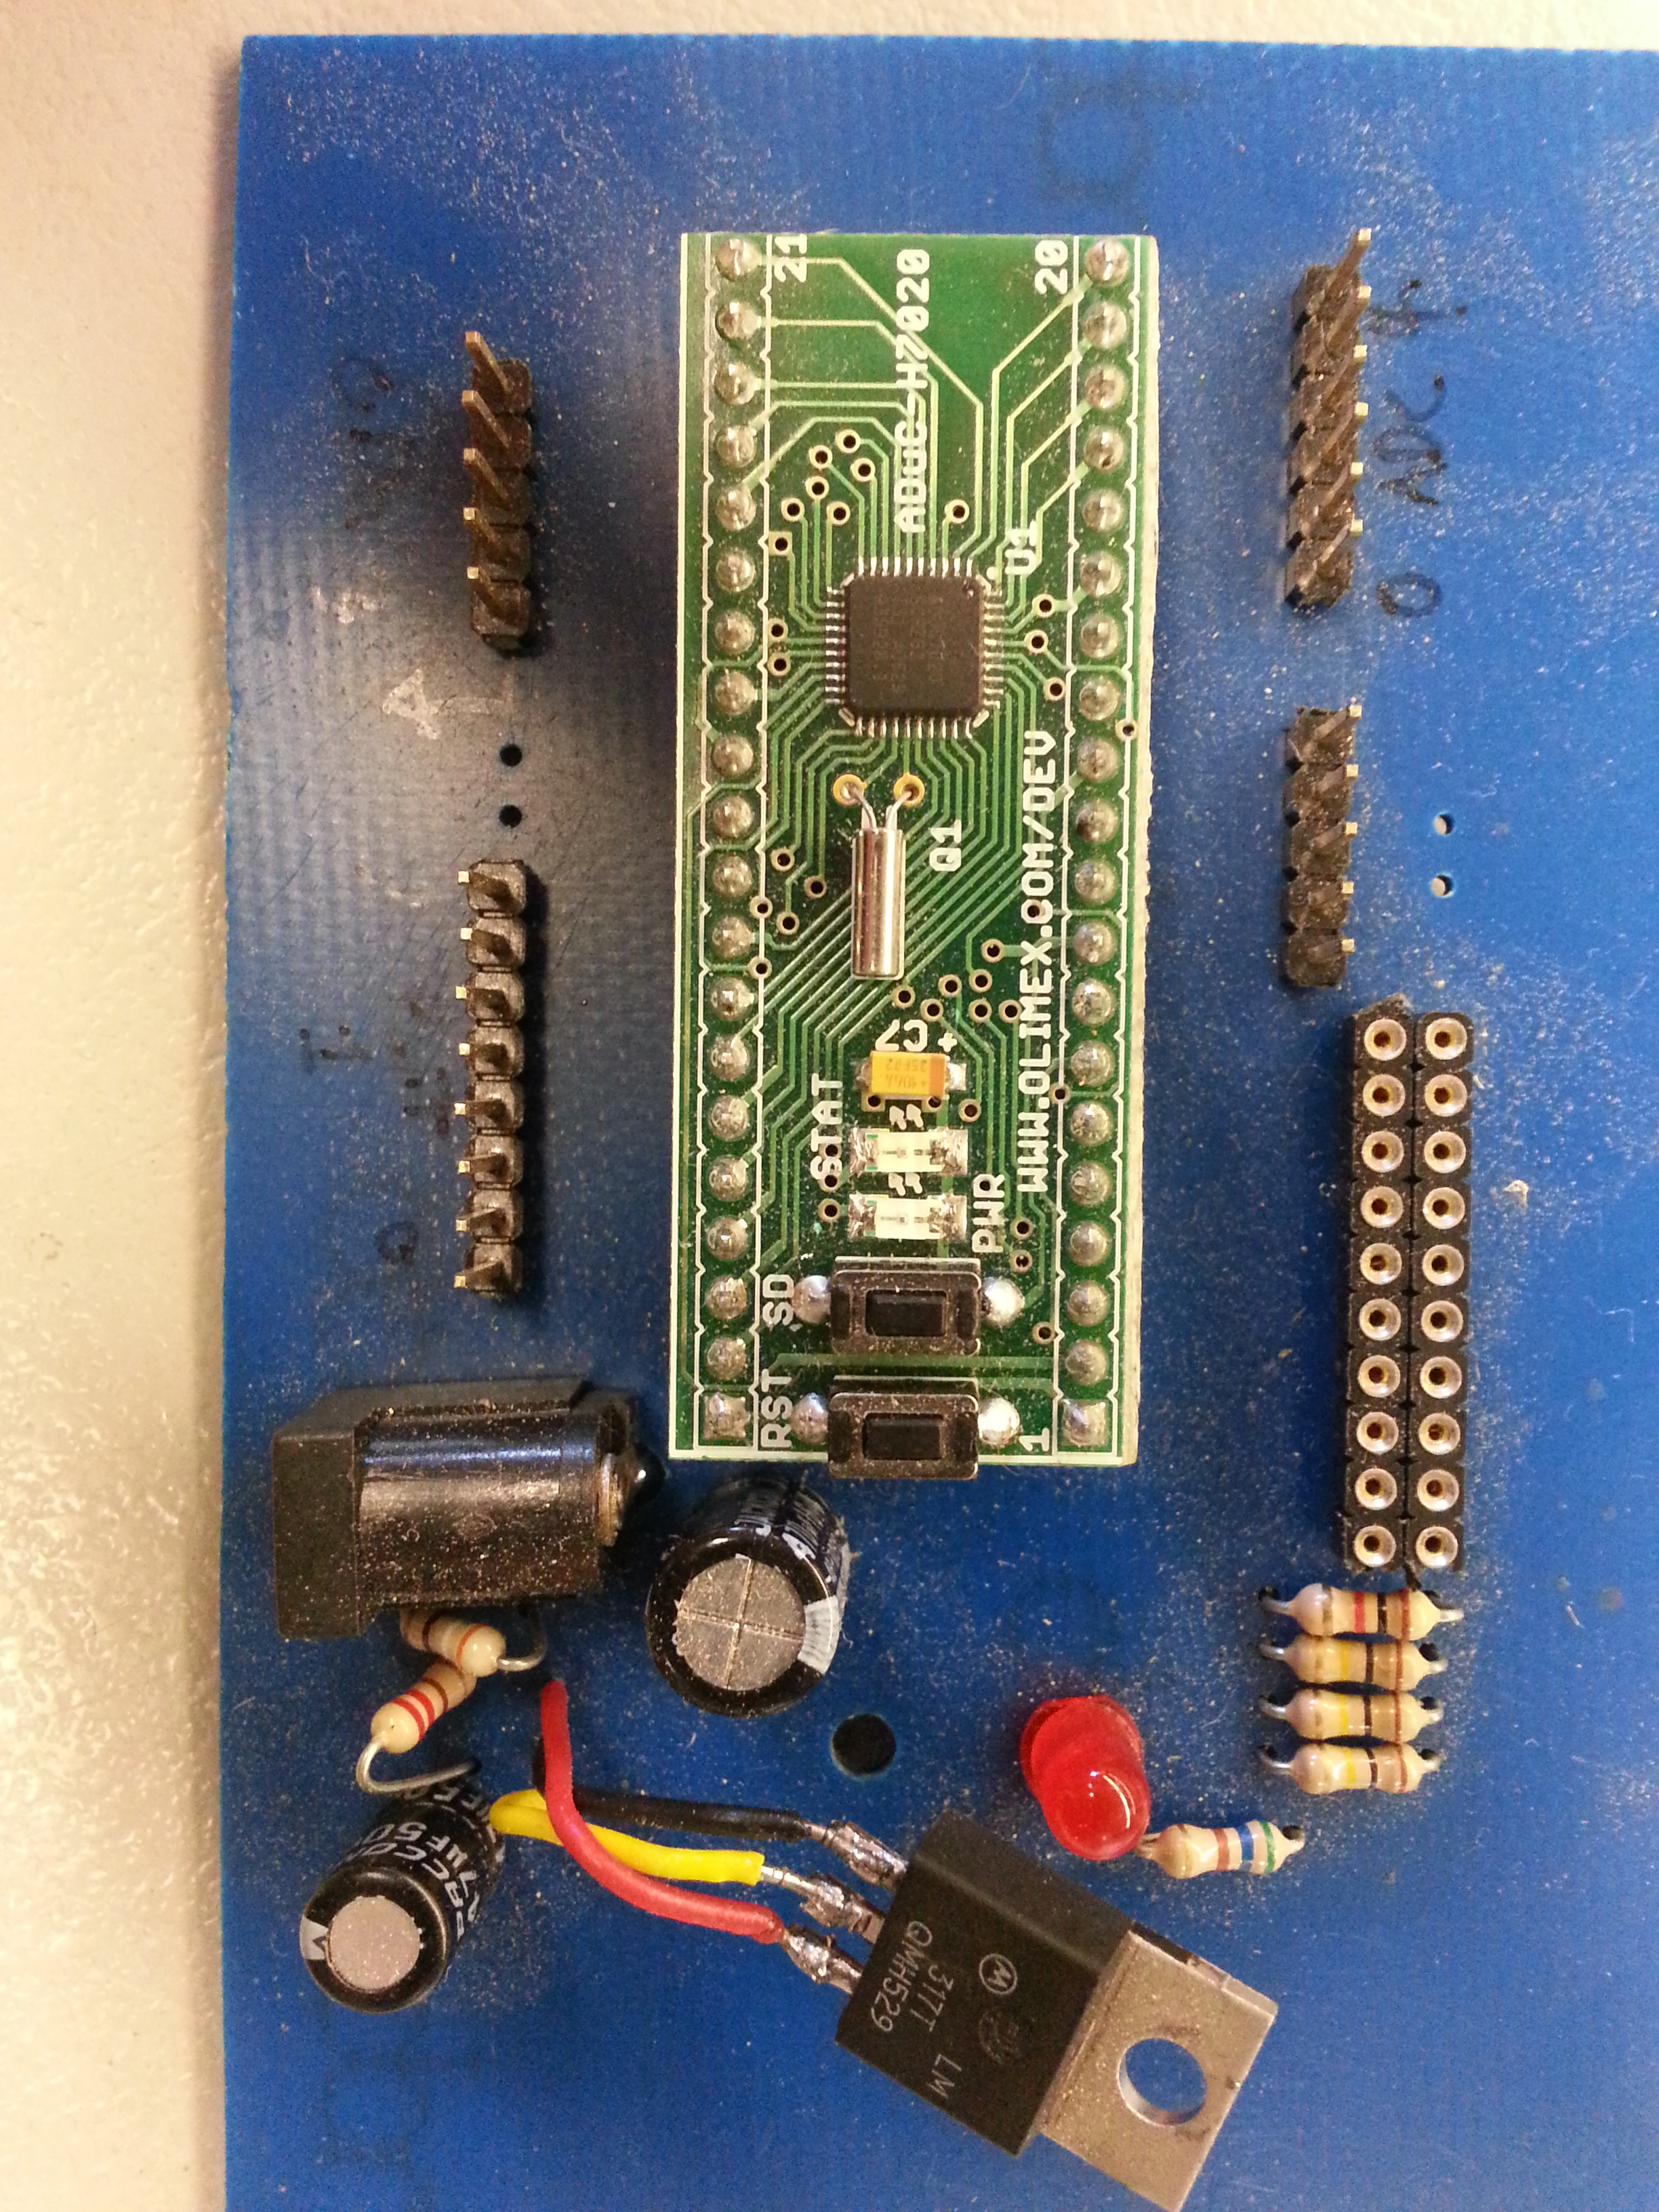
\includegraphics[scale=1,width=.45\textwidth]{Images/PCB_DigBetaA.jpg}
		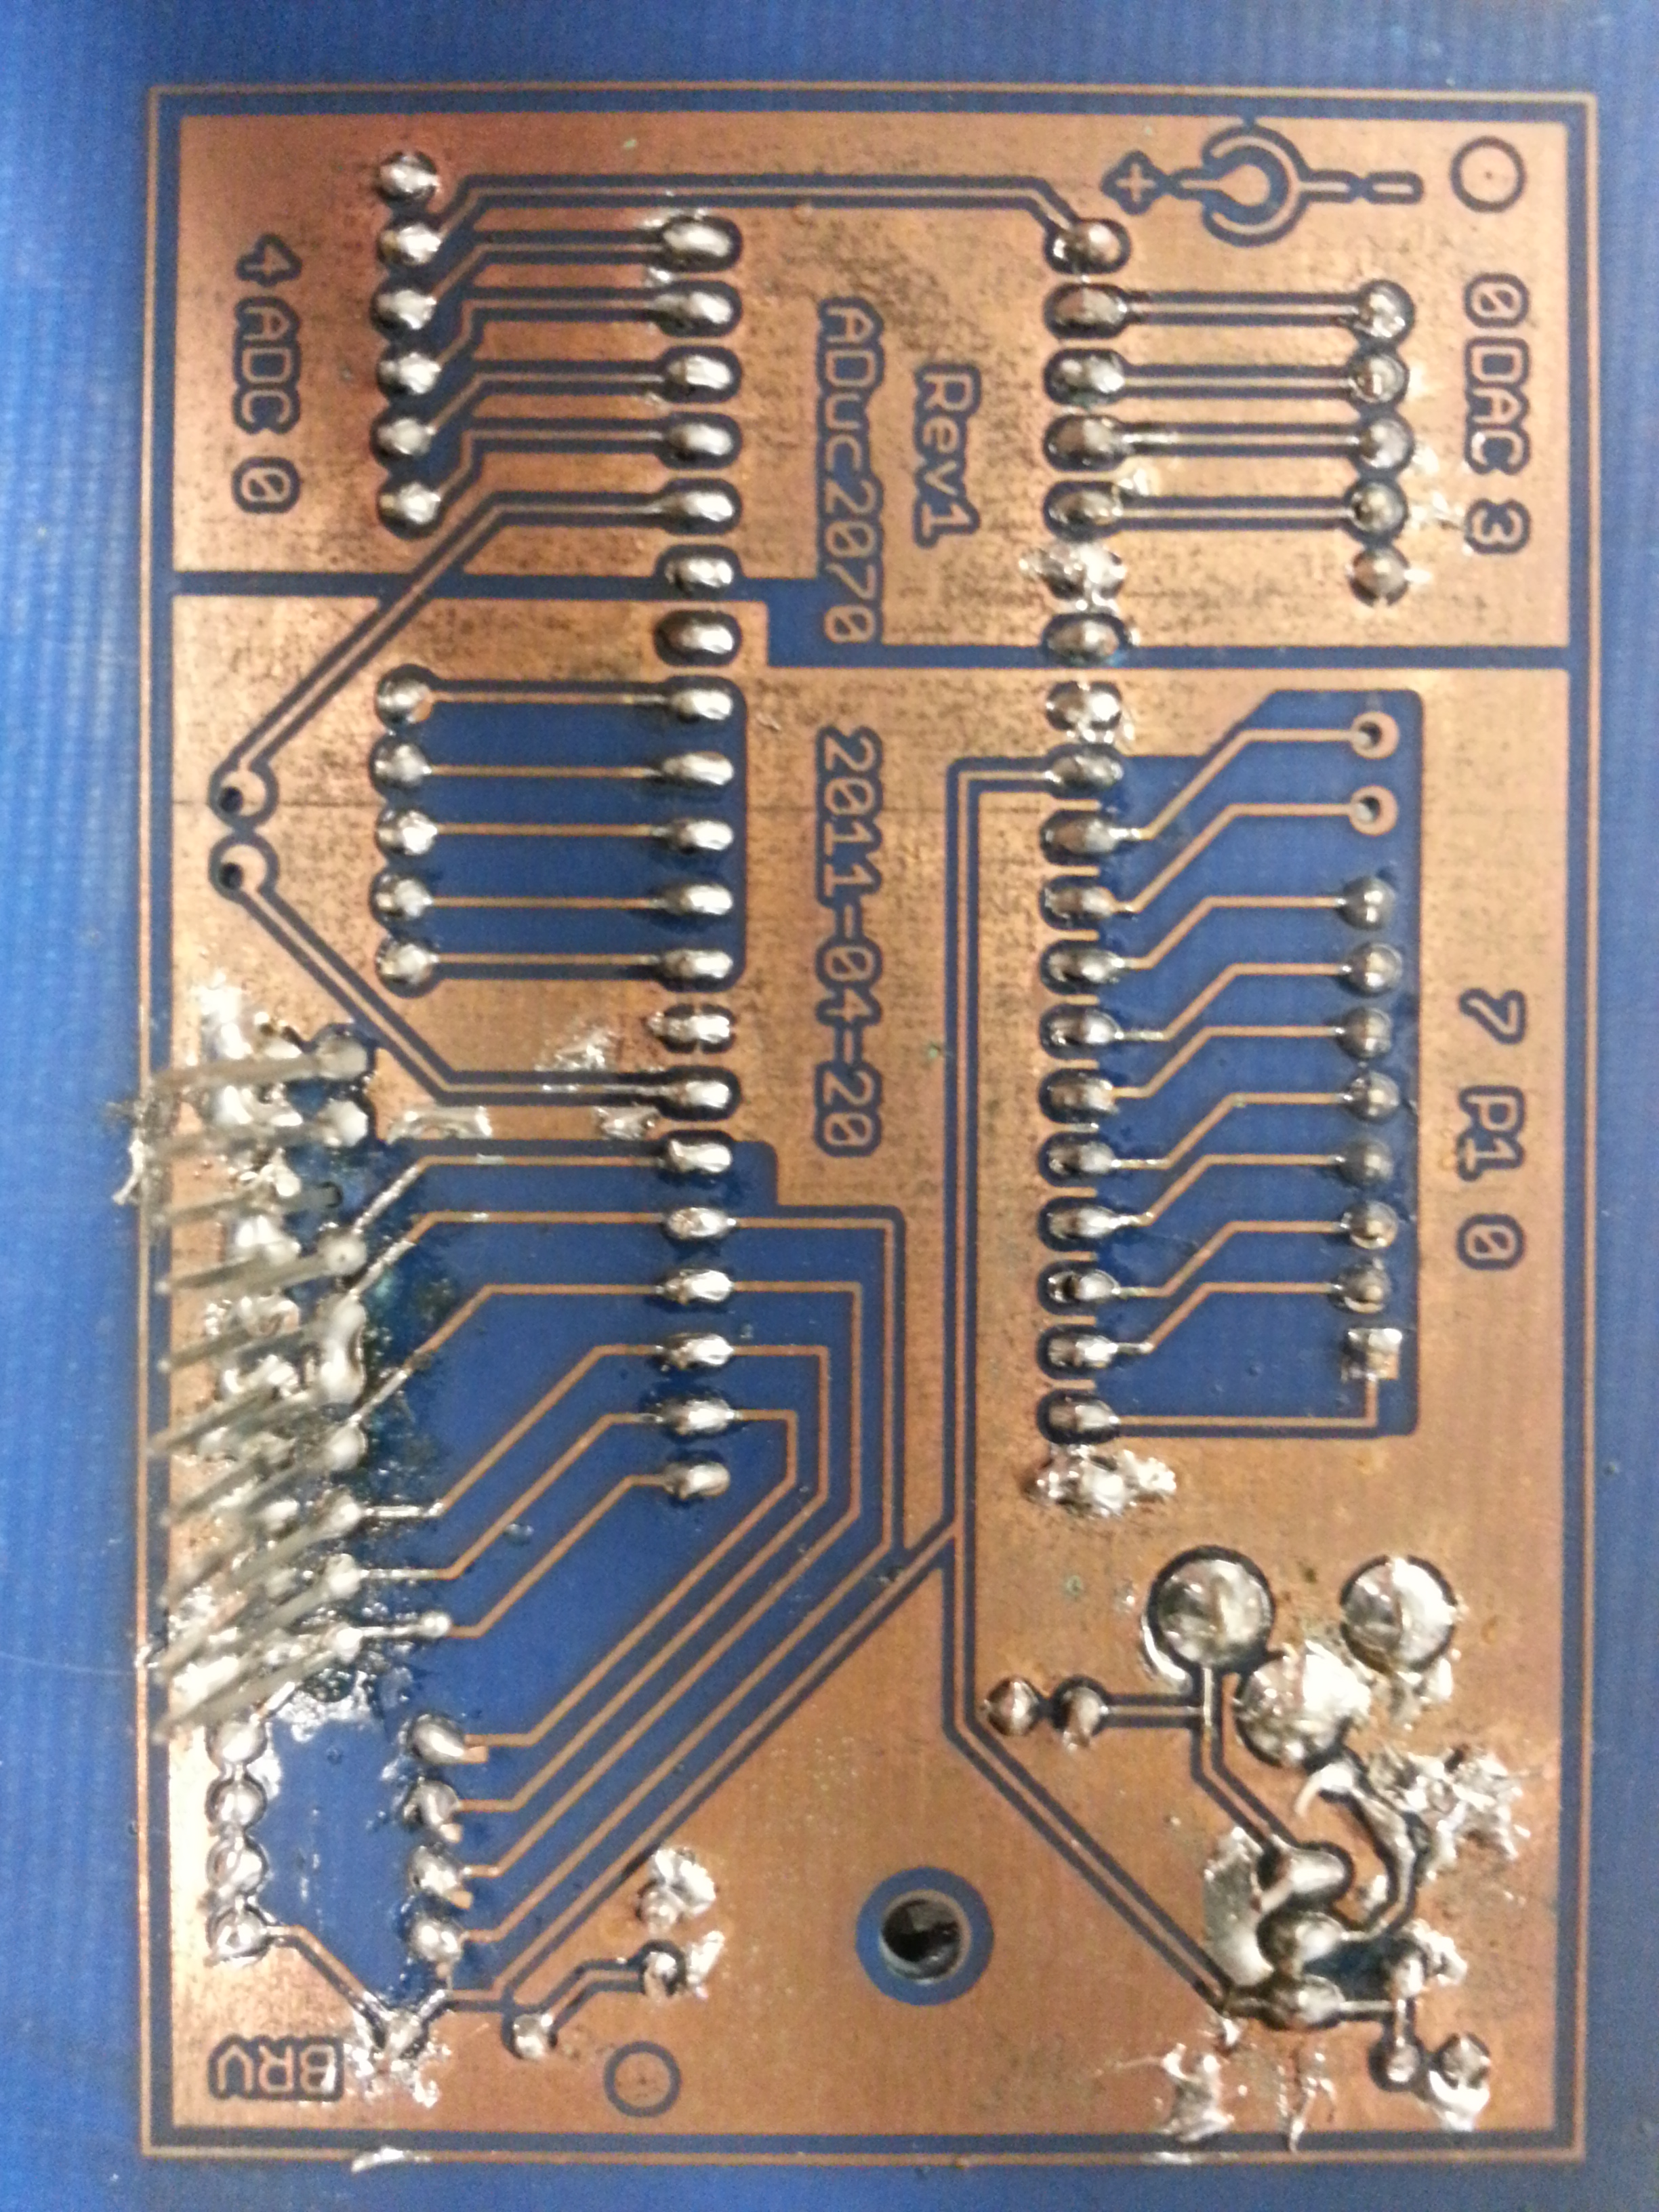
\includegraphics[scale=1,width=.45\textwidth]{Images/PCB_DigBetaB.jpg}  
		\caption{Beta Control Board}
		\label{fig:PCB_digital_beta}
	\end{center}
\end{figure}

To clarify the different parts of the design the hardware device was referred to as the Mobile Cardiac Heart Monitor (MCHM). This first revision, shown in \cref{fig:PCB_Rev1}, was designed as a test platform. It included many peripherals including an accelerometer, Bluetooth-communication, USB-communication, SD card storage, and an integrated  Lithium Polymer (LiPo) battery charger in addition to the previously designed analog front end. The board also transitioned to surface mount parts. This board was assembled and tested. Once basic functionality of all components was verified, We began to work towards miniaturization of the device. This effort would attempt to streamline the design; reducing points of failure, cost, complexity, and size.  Revision 2 (Rev2) was never manufactured due to a supplier mix-up. The processor had been advertised with an incorrect footprint. It was determined to be cheaper to have new boards manufactured using the altered footprint than to wait for new processor. The revised board was called revision 3 (Rev3), shown in \cref{fig:PCB_Rev3}, functionally identical to revision 2 but with a different microprocessor footprint. Rev3 added the feature of a connector that could easily be affixed to ECG leads without proprietary devices. Rev3 also could function as a full nine degrees of freedom sensor (9DOF). This was used for another researcher's master thesis [16]. Finally, a new \spo2 sensor was being developed by a master student, the original design was removed, and a header was added for connection to any design the student could create.

\begin{figure}
	\begin{center}
		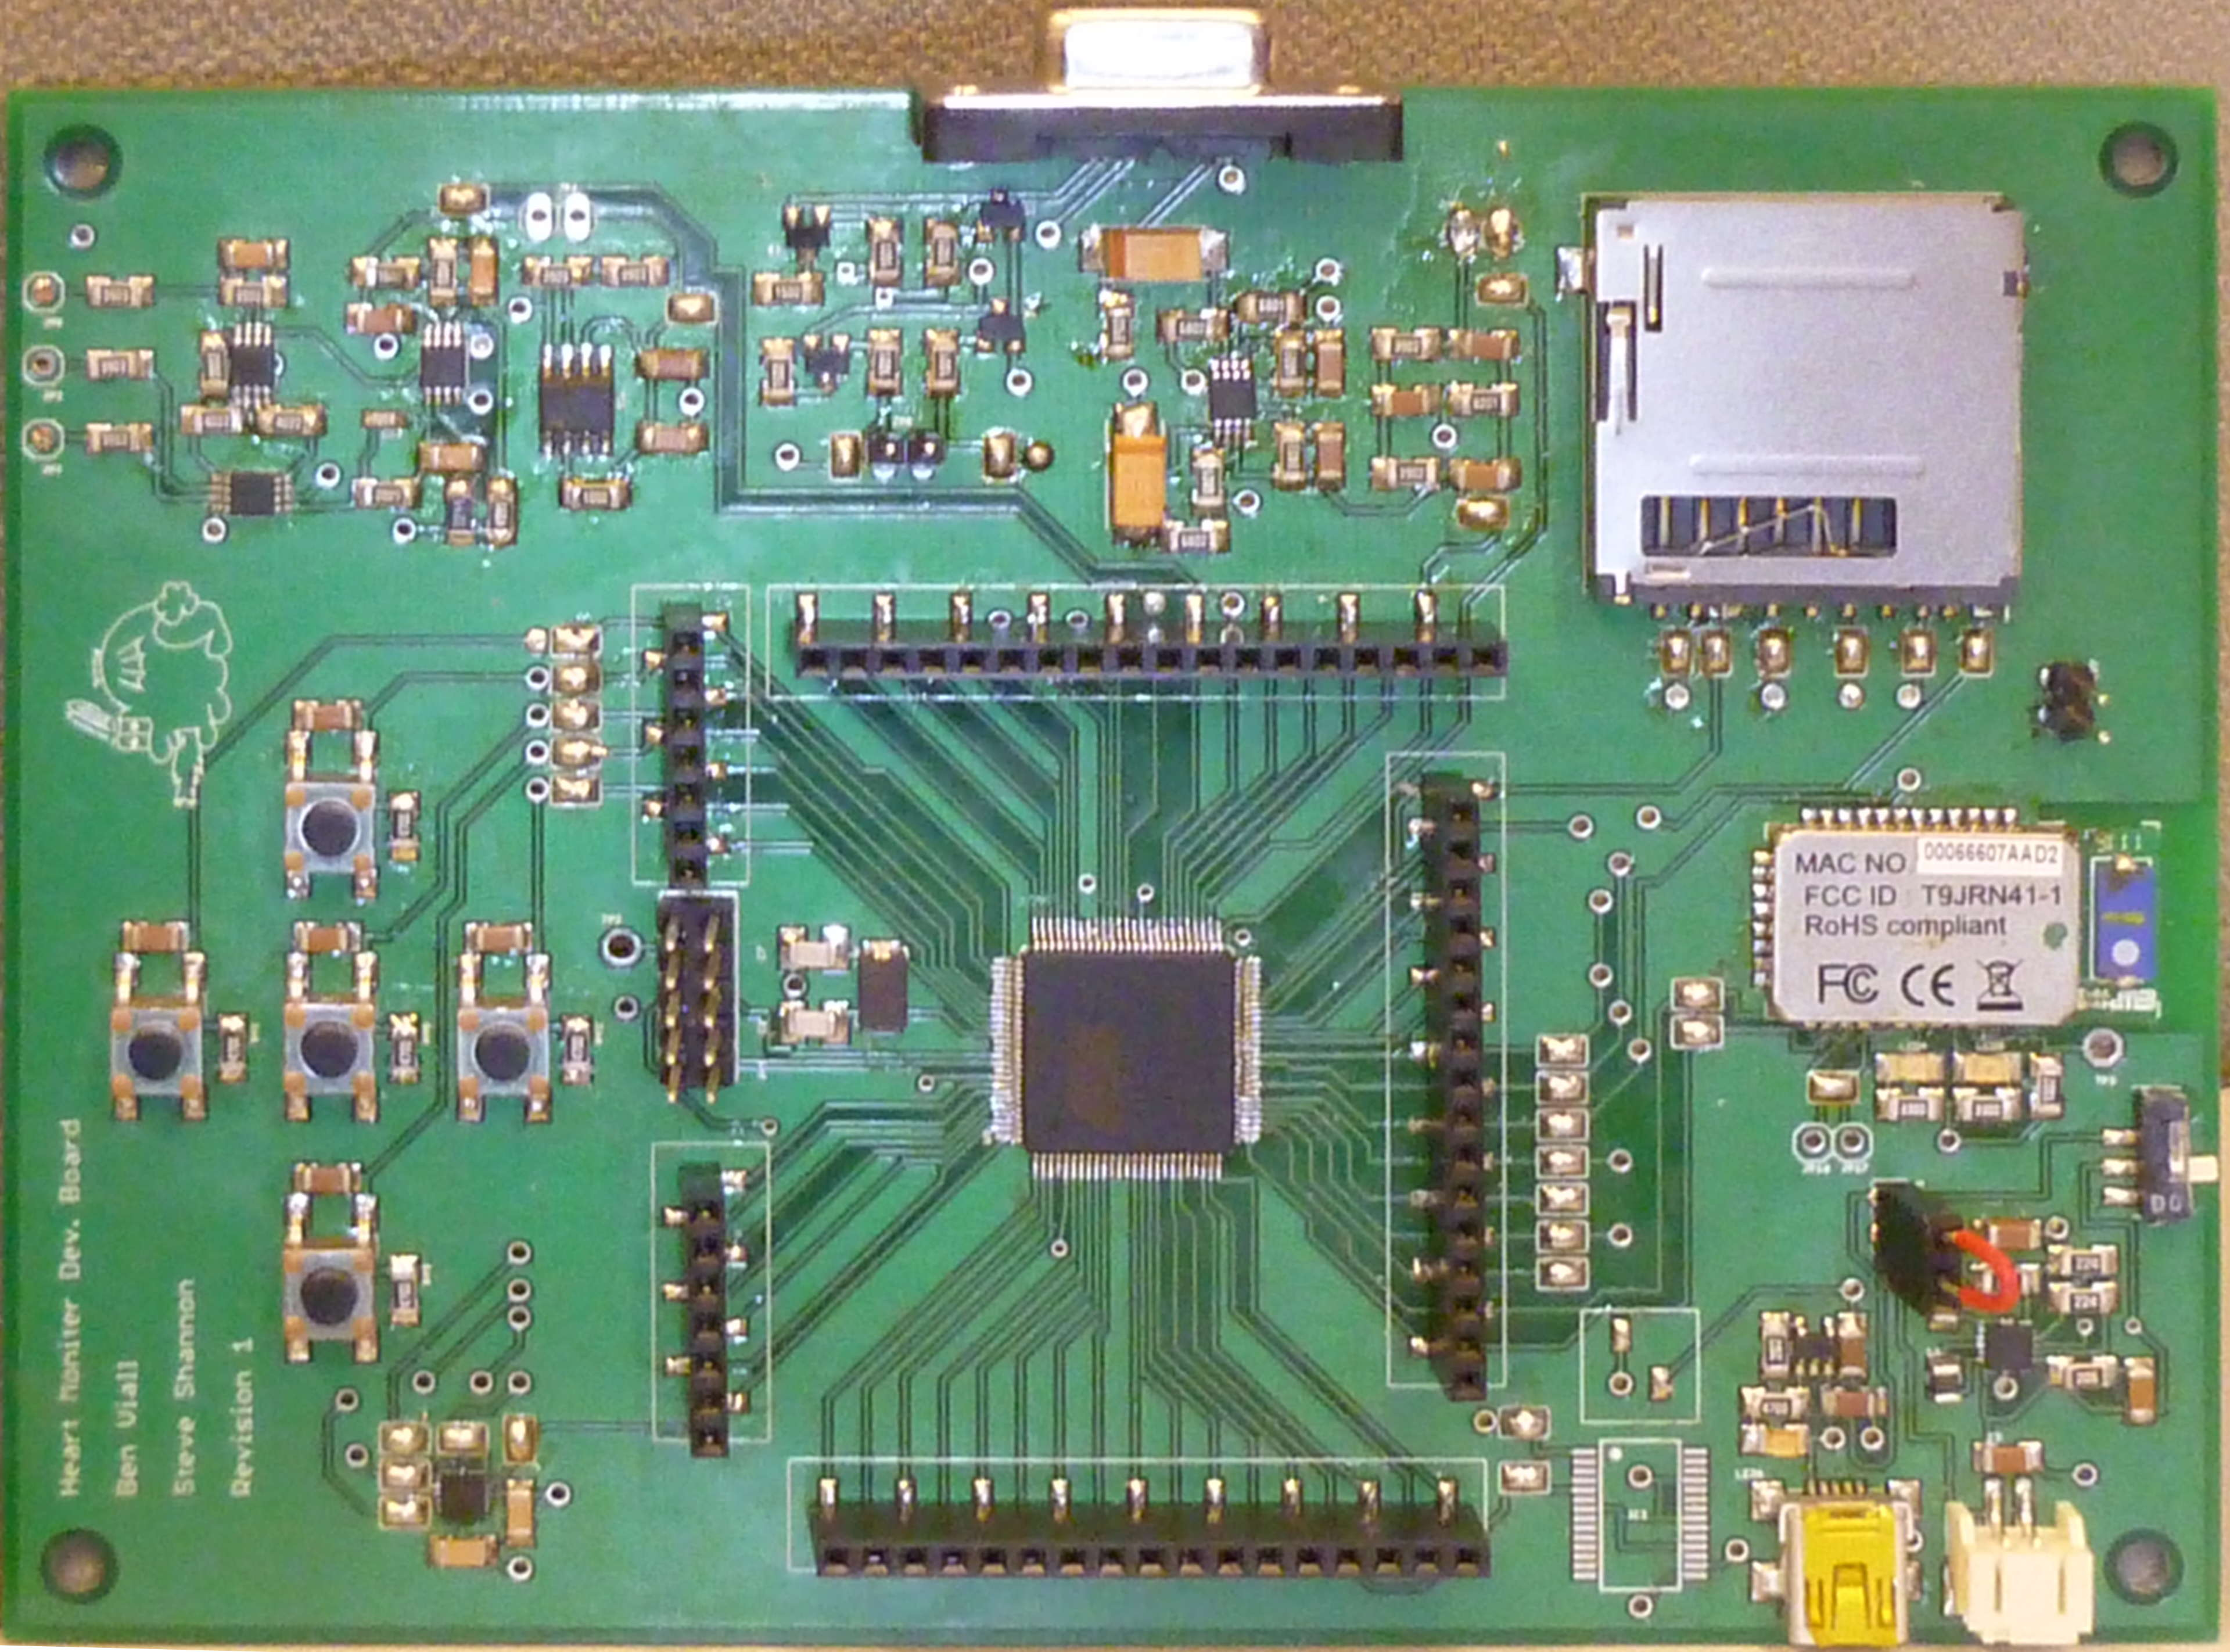
\includegraphics[scale=1,width=0.9\textwidth]{Images/PCB_Rev1.jpg} 
		\caption{MCHM PCB Rev 1}
		\label{fig:PCB_Rev1}
	\end{center}
\end{figure}


Currently we are working on new designs for both ECG and \spo2 analog front-end (AFE) circuitry. These new designs will offload much of the filtering to software reducing components and cost. A Texas Instruments app note discusses trade-offs concerning AFE complexity and ADC design. [55] They present two scenarios for ECG signal acquisition. First, a 16-bit or lower resolution is presented. Preparing a signal for capture by a 16-bit ADC involves a significant amount of front end analog processing as show in \cref{fig:SAR_topology}.\cite{Soundarapandian2010} At each stage of the AFE, additional noise is inserted into the system. Furthermore, the complexity of the AFE design can significantly drive up cost.

\begin{figure}
	\begin{center}
		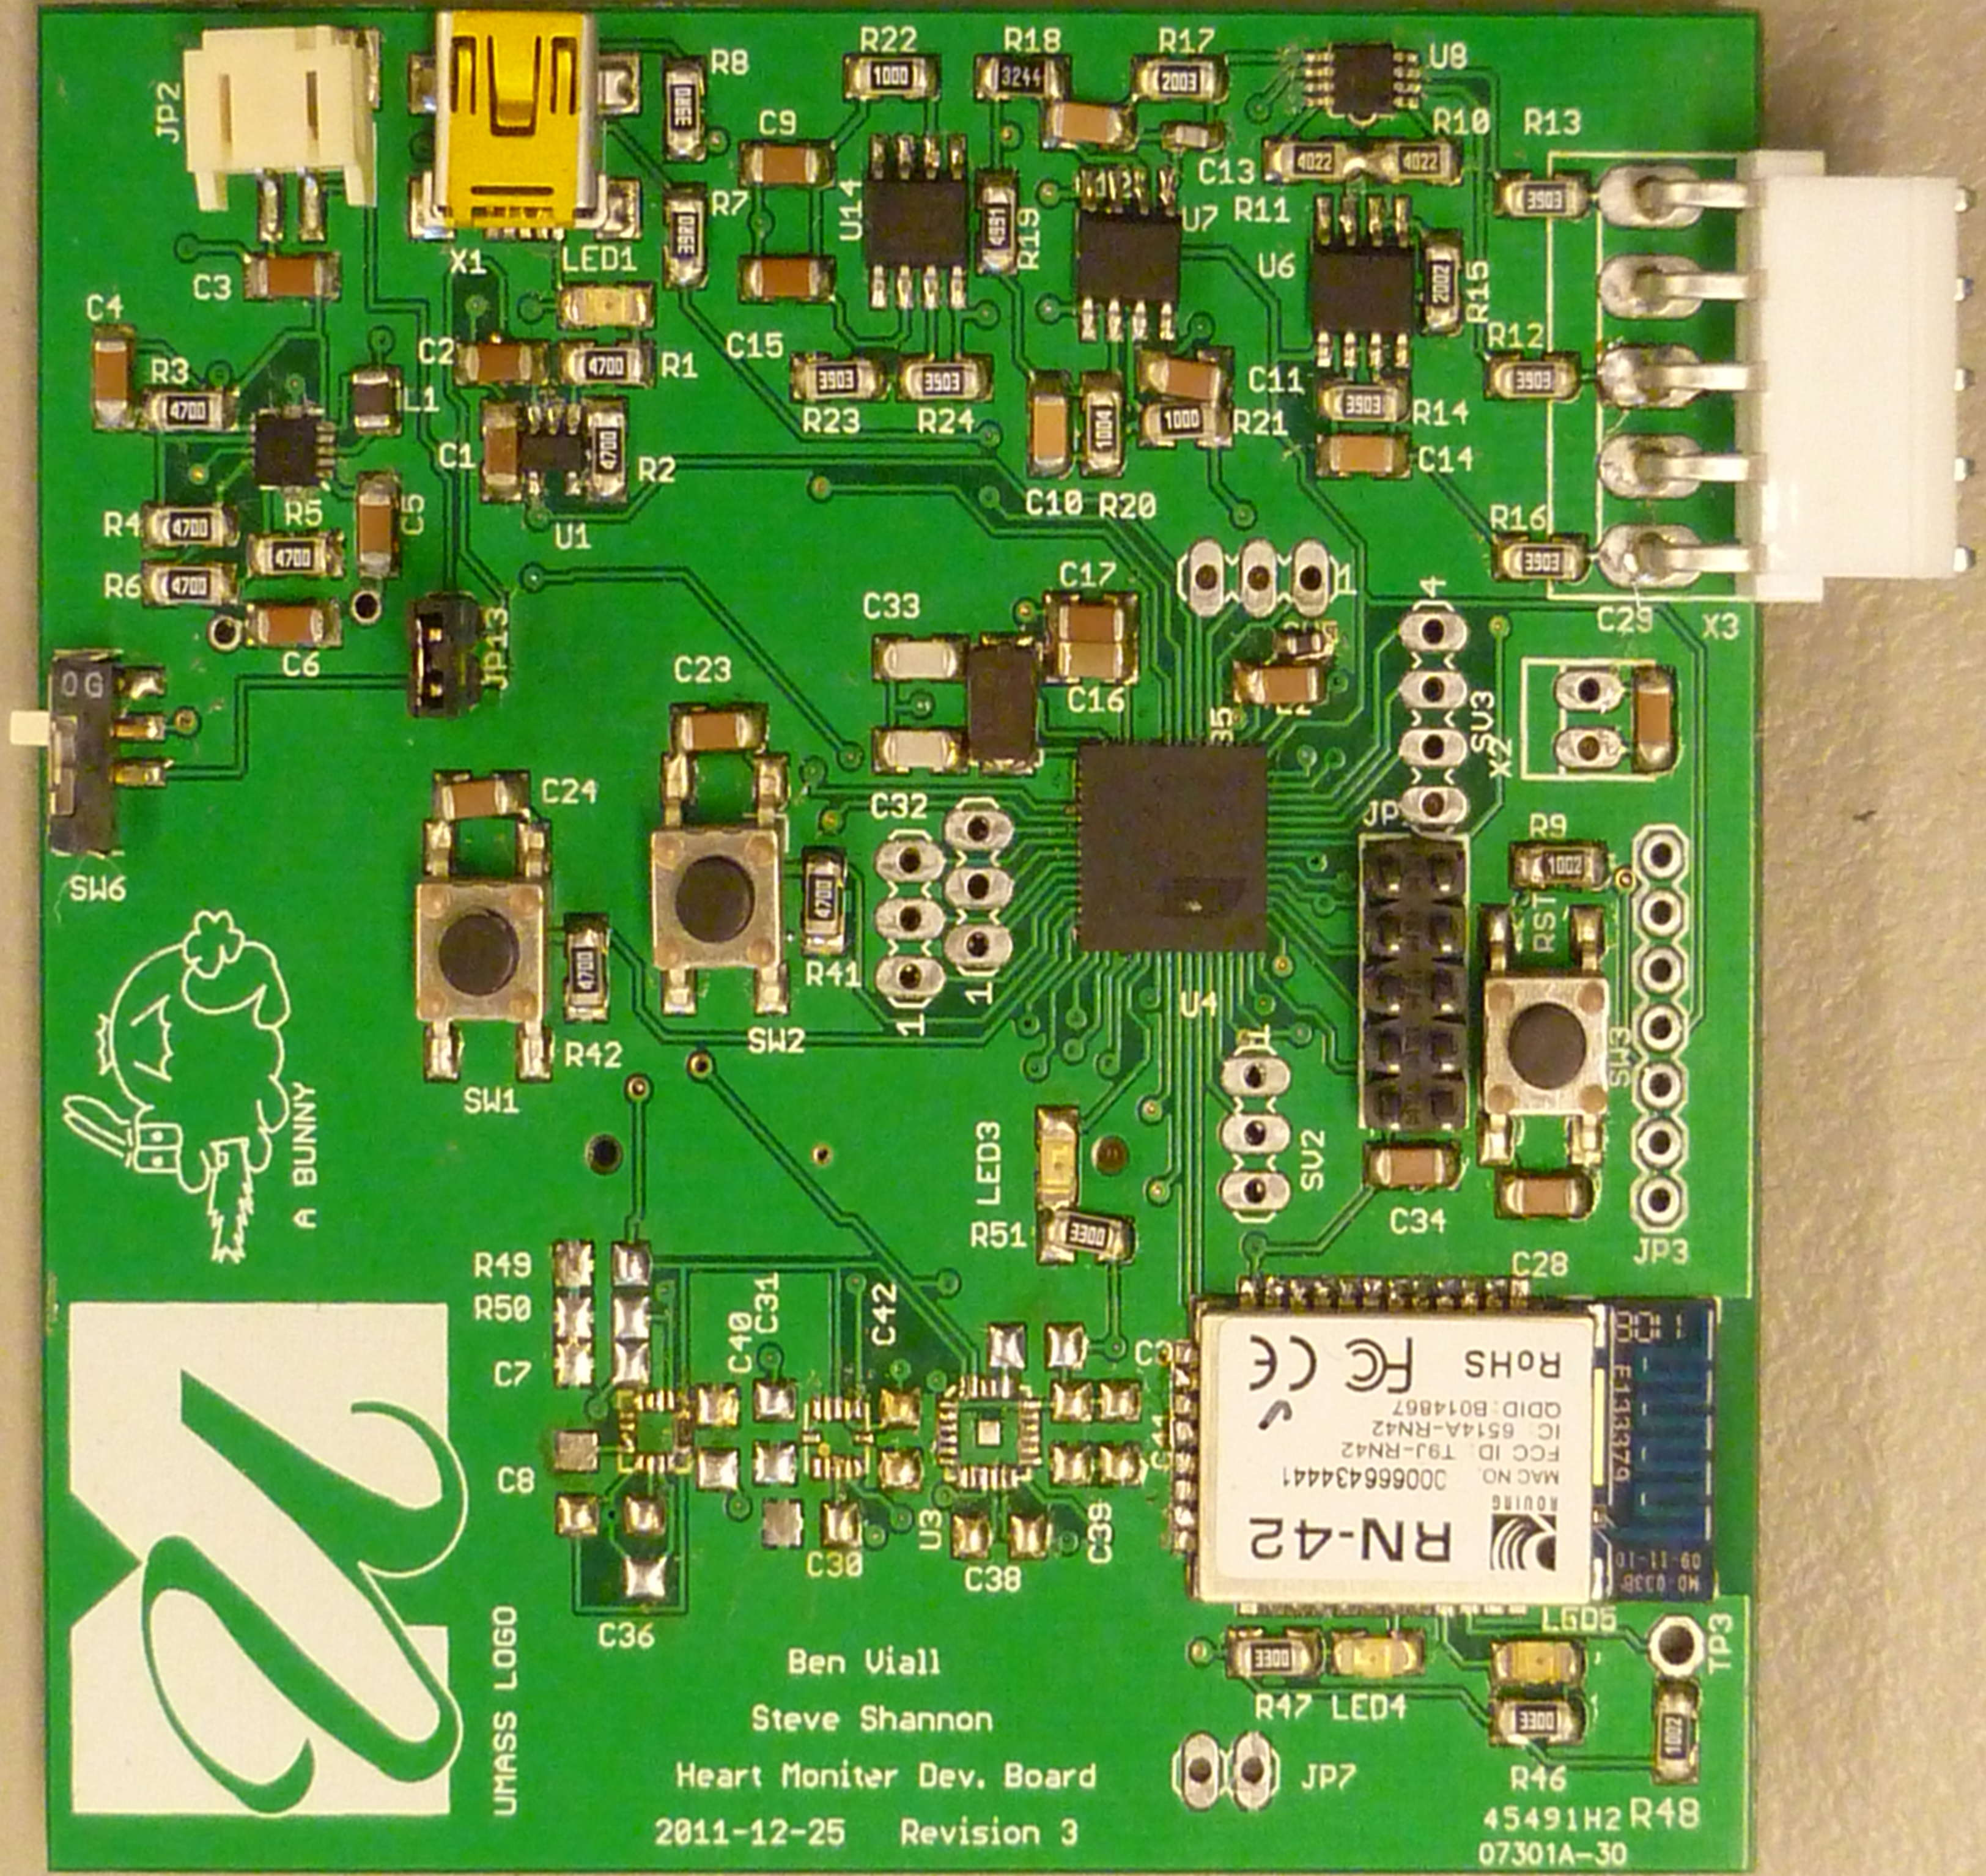
\includegraphics[scale=1,width=0.9\textwidth]{Images/PCB_Rev3.jpg} 
		\caption{MCHM PCB Rev 3}
		\label{fig:PCB_Rev3}
	\end{center}
\end{figure}

However, the application note presents an alternative, shown in \cref{fig:sigmaDelta_topology}. \cite{Soundarapandian2010} Given a 24-bit sigma-delta ADC, only a low gain instrumentation amplifier and first order passive filter are needed to prepare the signal for conversion.  This approach offers higher accuracy than traditional ECG techniques and keeps the baseline drift of the signal intact allowing for more flexibility in the digital signal processing. We are currently designing an AFE component to capture both the ECG and \spo2 readings using a $ \Sigma\Delta $ approach. Using the $ \Sigma\Delta $ approach simplifies future design problems. Designs can now have a simplified AFE and biometric signals can be filtered using simple to implement software filters using any hardware description language such as VHDL. This outcome is preferable to a fixed hardware design since it will allow more flexibility in the design stages. Adding additional features and filters need not increase hardware costs.


\begin{figure}
	\begin{center}
		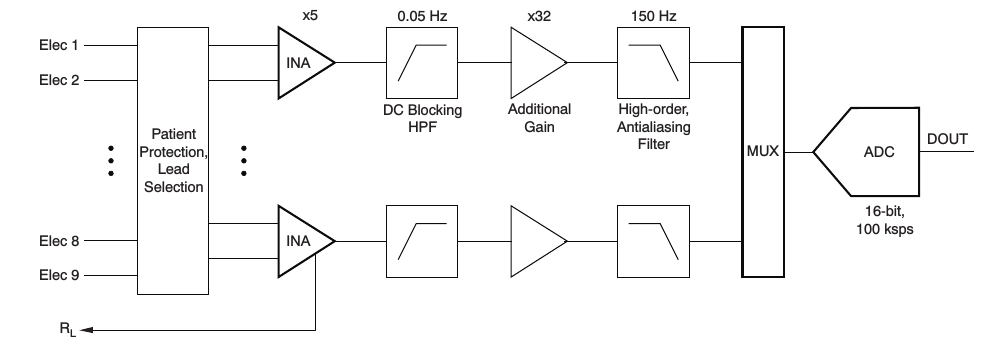
\includegraphics[scale=1,width=0.9\textwidth]{Images/SAR_topology.png} 
		\caption{Typical ECG Acquisition System }
		\label{fig:SAR_topology}
		\end{center}
\end{figure}

Other group research will be used as input to the dissertation. Previous, completed, master level research by Parma Chaiyasucheeva provided an elementary classification algorithm based on cardiac metrics\cite{Chaiyasucheeva2012}. Steven Shannon completed a master level thesis relating to fusing accelerometer data with other metrics and classifiers to combat movement artifacts\cite{Shannon2012}. Brendan Putin completed a master level project by creating a smartphone application to deliver psychosocial instruments and store the results in a database  \cite{Putin2011,Louro2013} Current work is being performed, under supervision, by master level candidates. Patrick DaSilva is working to classify ECG signals based on their components and continue Parma Chaiyasucheeva's work on patient wellness calculation. Alexander Ekholm is researching PPG sensor technologies. Specifically, design, implementation, and validation of a sensor capable of reflective PPG collection at a non-peripheral site, near the heart.  Also, under development, Brian Lauro is working on a minimal cardiac ontology, and BKE.

\begin{figure}
	\begin{center}

		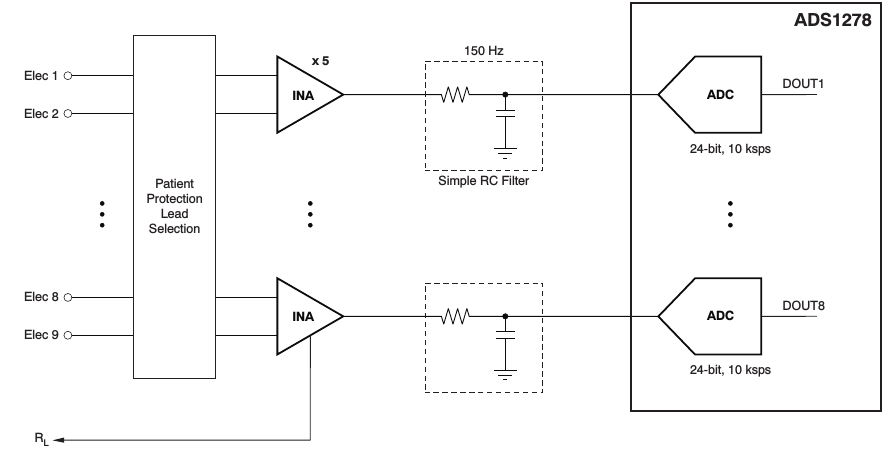
\includegraphics[scale=1,width=0.9\textwidth]{Images/sigmaDelta_topology_simultanious.png} 
		\caption{ECG Approach using $\Sigma\Delta $ ADC}
		\label{fig:sigmaDelta_topology}
	\end{center}
\end{figure}

\section{Description of Dissertation Chapters}

\subsection{\expandafter{\Cref{chap:introduction} \nameref{chap:introduction}}}
\label{subsec:Chapter1Introduction}
In the Introduction chapter, I will discuss the current state of medical care for CHF patients. I will present the relevant statistics about hospitalization and mortality. I will then cover the topic of engaging patients in their own self-care, citing relevant studies and statistics. Then finally indicate the proposed solution.

\subsection{\Cref{chap:LitReview} \nameref{chap:LitReview}}
\label{subsec:Chapter2LitReview}
This section will first cover previous research done in the fields of ECG, \spo2 /PPG, and acceleration sensors. Then a discussion of how to derive synthetic sensor measurements based on acquired ECG, \spo2 /PPG, and acceleration measurements. I will focus on literature with methods of deriving heart rate, blood pressure without an inflatable cuff, and deriving respiration rate without a chest strap. Next, I will present methods for removing noise from the ECG and PPG sensors based on accelerometer data. Finally, the pertinent literature in the medical domain will be reviewed, paying specific attention to the fields of patient education and self-care as well as the psychosocial instruments to be used, the MLHF, DASI, and HFSA.

\subsection{\Cref{chap:trialResults} \nameref{chap:trialResults}}
\label{subsec:Chapter3SystemDesignConcepts}
In \cref{chap:trialResults} I will discuss the trial protocol, and lessons learned during and after the exploratory trial.

\subsection{\cref{chap:ProtoTypeBuildTest} \nameref{chap:ProtoTypeBuildTest}}
In \cref{chap:ProtoTypeBuildTest} I will discuss the hardware design decisions and prototype assembly, testing, and validation of the WHIP Sensor platform. I will address various hardware decisions I encountered while designing the senor suite and its communication with the smartphone app. I will also address power usage of the device and any layout related board issues. Finally, I will address the packaging of the device into a wearable sensor.

\subsection{\Cref{chap:SensorConcepts}  \nameref{chap:SensorConcepts}}
In this chapter, I will cover in detail the code and firmware techniques used in the data flow of the sensor designs covering both the analog front end for the real sensors in the WHIP.

\subsection{\Cref{chap:conclusions} \nameref{chap:conclusions}}
\label{subsec:Chapter8Conclusions}
Validating my system with an exploratory study is only the first step in a larger design philosophy. I will indicate avenues of improvement for hardware and software focusing on moving to a system on a chip (SoC) design. I will present my conclusions and suggest future steps in the research.



\chapter{Literature Review}
\label{chap:LitReview}
%This section will first cover previous research done in the fields of ECG, SpO2/PPG, and acceleration sensors. Then a discussion of how to derive synthetic sensor measurements based on acquired ECG, SpO2/PPG, and acceleration measurements. I will focus on literature with methods of deriving heart rate, blood pressure without a cuff, and deriving respiration rate without a chest strap. Next, I will present methods for removing noise from the ECG and PPG sensors based on accelerometer data. Finally, the pertinent literature in the medical domain will be review, paying specific attention to the fields of patient education and self-care as well as the psychosocial instruments to be used, the MLHF, DASI, and HFSA.

\section{Prior Research}
\label{sec:priorResearch}
There are numerous related research areas affecting our proposed work. Loosely the related research areas are existing standards (e.g. sensors, wireless, heath, and health ontologies.), physical and synthetic sensors, data fusion and classifications. In the following sections, each is briefly examined in relation to our research effort.

\subsection{Existing Standards}
\label{sebsec:ExistingStandards}
In order to promote adoption of the WHIPPED system, sensor standards, wireless-standards, healthcare-standards, and health ontology-standards are examined. Sensor standards are examined that may affect the design of the sensor patch. Wireless standards are examined to determine the best way to transmit biometric data to the cell phone. Finally, health standards, and health ontology-standards are examined to find trends in the storage, transmission, and classification of health information and disease classification.

\subsubsection{Sensor Standards}
\label{subsec:SensorStandars}
Data from the sensor suite must be interpreted by the control microprocessor and transmitted to the patient's phone consistently. Different protocols for sensor data interpretation and transmission already exist.  The Open Geospatial Consortium Inc. (OGC) is developing an initiative called Sensor Web Enablement (SWE) \cite{Botts2007a}. SWE is a collection of open standards designed to make any type of sensor plug and play. SWE is made up of several standards such as Sensor modeling language (SensorML) \cite{Botts2007}, and Transducer modeling language (TransducerML), among others. SensorML represents a standard way for providing specifications for a sensor device. Only a subset of the large amount of metadata provided by SensorML is needed. TransducerML defines a self-describing protocol based on XML to support data transmission between any type of sensor and data sink \cite{Fortier2009}.

These standards propose a heavyweight approach to sensor identification and interoperability. SWE allows any sensor to be seamlessly integrated into a system. Our research approach is to use a fixed set of sensors. The high overhead of SWE makes it unsuitable for our research. However, meta-data concerning the transducers is still needed. We propose a more lightweight approach using IEEE standard 1451.4, Transducer Electronic Datasheets (TEDs) . For most smart transducers, TEDS uses a memory device attached to the transducer, which describes the transducer's identification, calibration, correction data, measurement range, manufacturer related information, and so on. TEDs allow us to be relatively free with our hardware choices by allowing our software to read the required information from the sensor patch. Many versions of the sensor patch hardware can integrate seamlessly with one software platform by providing the TEDS.
%$\cite{#IEEE1451_4}$

\subsubsection{Wireless Standards}
\label{subsubsec:WirelessStandards}

\begin{figure}
	\begin{center}
		\label{fig:WirelessComparison}
\begin{tabularx}{1\textwidth}{>{\bfseries}p{.23\textwidth}||p{.25\textwidth}|p{.15\textwidth}|p{.25\textwidth}}
\hline Standard 			& Wi-Fi & Bluetooth & ZigBee \\ \hline
\hline IEEE Spec. 			& 802.11 a/b/g & 802.15.1  & 802.15.4 \\ 
\hline Frequency Band 		& 2.4 GHz; 5 GHz & 2.4 GHz & 868/915 MHz\par2.4 GHz \\ 
\hline Max \par Signal Rate 		& 54 Mb/s & 1 Mb/s & 250 Kb/s \\ 
\hline Nominal Range 		& 100 m & 10 m & 10 – 100 m  \\ 
\hline Nominal TX Power 	& 15 – 20 dBm & 0 – 10 dBm & (-25) – 0 dBm \\ 
\hline Number Of RF Channels & 14 (2.4 GHz) & 79  &  1/10; 16\\ 
\hline Channel \par Bandwidth 	& 22 MHz & 1 MHz  & 0.3/0.6 MHz; 2 MHz \\ 
\hline Coexistence Mechanism& Dynamic freq. selection, transmit power control (802.11h) & Adaptive freq.\par hopping & Dynamic freq. \par selection \\ 
\hline Maxi. nodes & 2007 & 8 & 65000 \\ 
\hline Encryption 			& RC4 stream cipher (WEP),\par AES block cipher & E0 stream cipher & AES block cipher \par(CTR, counter mode) \\ 
\hline Authentication 		& WPA2 (802.11i) & Shared secret & CBC-MAC \par(ext. of CCM) \\ 
\hline Data Protection 		& 32-bit CRC & 16-bit CRC &  16-bit CRC\\ 
\hline 
\end{tabularx} 
		\caption{Comparison table of wireless technologies}
	\end{center}
\end{figure}


Collecting, and interpreting, sensor data is only part of the problem statement. To be useful a device must transmit data for further processing. Several standards and architectures for data transmission were considered. A wired connection to a cell phone was quickly discarded. While it would offer a simple and fast communication to a comparatively more powerful device, it is obtrusive and introduces a hazard to movement that could exert a strain on both devices if the cable became caught on another object. Therefore, several methods of wirelessly transmitting our collected data were researched. Several technologies make use of the ISM 2.4 GHz band; Bluetooth, ZigBee and Wi-Fi fall into this category and were examined.  Shannon compares Wi-Fi, Bluetooth, and ZigBee in his master's thesis \cite{Shannon2012}. Wi-Fi offers the highest throughput and range but at the cost of extreme power usage. Bluetooth has the next highest throughput at much more acceptable power consumption. ZigBee offers the most customization and is capable of supporting up to 65000 devices in a single network, however is lacks cell phone communication support.

While ZigBee meets our minimum bandwidth requirement, as shown in \cref{WirelessComparison}, and uses less power, Shannon concludes the lack of smart phone hardware support makes Bluetooth a better option presently. In the future, if phones begin supporting the ZigBee protocol a switch could be made.  ZigBee could be a viable protocol in the future as shown by Peligris; who examines the IEEE802.15.4, the protocol underlying ZigBee \cite{Pelegris2011}.

Bluetooth is a wireless technology standard for exchanging data over limited distances. It supports many profiles including: hands free profile a stereo audio profile, and serial port profile. Noueihed et al. compare two profiles for the transmittance of biometric data. The Serial Port Profile (SPP) is compared to the recently released Health Device Profile (HDP). The results of the analysis indicate HDP offers better reliability in some cases of interference, episodic transmission interference, and equal reliability in others, voice type interference \cite{Noueihed2010}. However, hardware support for HDP is currently scarce while support for SPP is nearly universal in Bluetooth modules. For the remainder of the dissertation Bluetooth SPP will be used. However, the application shall be designed modularly with the transition to HDP planed when better hardware support is available.

A primary driver in our analysis is the Space, Weight, and Power and Cost (SWaP-C) of the selected protocols and hardware support. Wi-Fi offers an unacceptably high power requirement. ZigBee offers no hardware support for our platform. Bluetooth SPP offers an acceptable power requirement and suitable data transmission rate.

\subsubsection{Health Standards}
\label{subsubsec:HealthStandards}
Usually if a patient receives home care services, they are seen within one week and the interval is determined by the nurse responsible for the patient. Home care patients are typically followed for at least 90 days depending on how sick they are. A nurse is sent to the patient's home to assess the patient's status. Between discharge and the first in-home visit, the patient does not interact with health care providers unless they seek assistance from their local primary health care provider. Gustafsson shows 25\%-50\% of hospitalized patients will be readmitted within six months of their initial hospitalization \cite{Gustafsson2004}. Further, Lee et. al would seem to indicate 25\%-30\% of CHF patients will die or have another hospitalization within the first 30 to 60 days \cite{Lee2011}. Lee and Gustafsson's findings underscore the need for better communication during those crucial first days and weeks after a patient leaves the hospital.

Agreeing on a common frame of reference is an essential part of the communication between clinician and patient.  Frequently elderly patients ignore symptoms of CHF because they attribute the pain(s) to “getting older” and not as a sign of a deteriorating condition. Several psychosocial and symptom tools have been produced enabling patient assessment by asking simple questions ranked on a likert -1 to five, scale. The Duke Activity Status Index (DASI) is a 12-item questionnaire with a score which can be translated into an estimated peak oxygen intake in mL/min \cite{Hlatky1989}. More commonly, the DASI is an indicator of energy levels used and is a general measure of activity.  Often patients with heart failure will decrease activities in the presence of worsening symptoms. Therefore, looking at the pattern of activity levels and symptoms provides a fuller picture of the patient's cardiac status. The Minnesota Living with Heart Failure Questionnaire (MLHFQ) is a 21-item questionnaire also using a likert scale \cite{Jurgens2009}. The MLHF-instrument measures patients' perceived QOL, and how much symptoms interfere with QOL. Repeated responses the MLHFQ strongly correlate to the New York Heart Association's (NYHA) classifications. The Heart Failure Somatic Awareness Scale is a 12 item likert scale developed to measure somatic awareness of and perceived severity of symptoms specific to heart failure \cite{Jurgens2006}. All of these instruments can be used to augment and correlate with the biometric readings collected by the sensor device. In addition, repeatedly administering these assessments can track changes in the self-perceived status of a patient. Establishing how patients perceive their own wellness is an important factor in treatment. In addition, educating a patient about the differences between their perceived status and actual status can be useful in a patient's self-care and rehabilitation.

In our research, we intend to use primarily the HFSA, DASI, and MLHF as instruments. The focus of our work is not development or validation of these instruments; that has been done in previous studies over an extended period, with thousands of patients.

\paragraph{Electronic Health Records (EHR)}
\label{par:ElectronicHealthRecords}
Some of the most important medical standards are still being written. An electronic health record (EHR) is a way of representing, and storing digitally, every medical piece of information about a patient. Data can be anything from patient demographics to an MRI scan or ECG data, temperature, weight, etc. The American Medical Informatics Association (AMIA) is working on developing a standard set of components for an EHR. Another, standard under development involves how information of various formats should be transmitted across different EHR systems. Both ANSI-X12 and HL7 are developing standards for electronic data interchange. When completed, an EHR will be a longitudinal record of every interaction a patient has had. The use of a subset of the EHR standard, mostly concerning the demographics of a patient and any history of heart disease and co-morbid illnesses will be sufficient for current research.

\paragraph{Health Ontology}
\label{par:HealthOntology}
When a clinician is diagnosing a patient, they often refer to clinical practice guidelines (CPGs). CPG are documents written for clinicians that provide evidence-based best practices. Given a set of symptoms, and patient demographics, a course of care can be prescribed to achieve a desired outcome. A full medical ontology would provide an exhaustive list of the domain of symptoms correlated with all possible demographic data and provide options for improving patient's conditions. A minimal database would be more than is necessary for our research.

Jones et al. show a method of converting a CPG to an XML based representation aimed at generating tailored educational material for clinicians [10]. A large portion of development time was spent generating the educational material and converting the CPGs to a computer format.  Many other approaches to representing CPGs electronically have been proposed, including EON, GEODE-CM, N-CODES and the Asgaard project. Shah proposes one additional method, Proteus. Proteus method focuses, not on the initial creation of the ontology but, on the maintenance, modification, and updating of the ontology.  By providing the ability to easily edit a large database of knowledge Shah suggests using a system such as PROTEUS will promote faster adoption of electronic health ontologies [11].

In our research, we are using a partial health ontology focused on chronic cardiac patients. The ontology supports definitions of symptom and symptom-severity, classifications of patients into the New York Heart Association's classes, appropriate interventions, and co-morbidity diseases. The intent is to aid in fast classification of patients and to detect patients in outliers.


\begin{figure}
	\begin{center}
		\label{fig:20SecondEcg}
		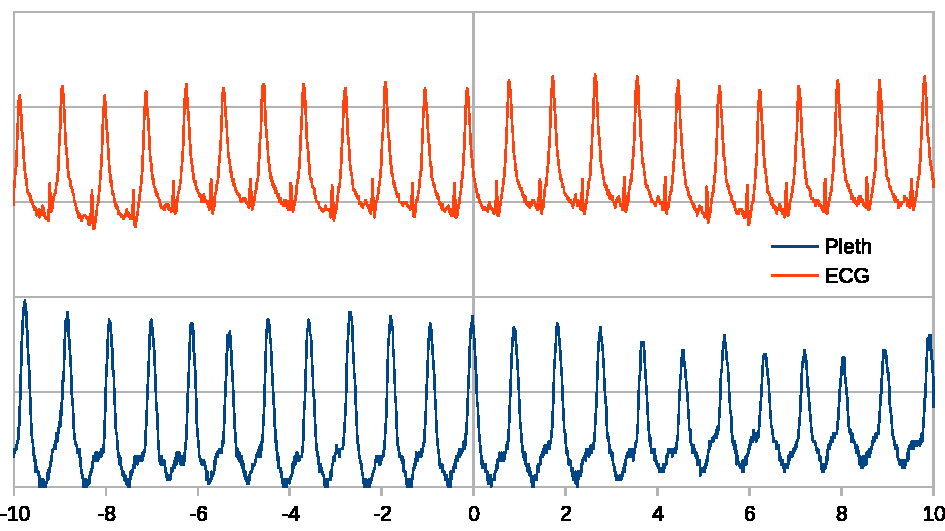
\includegraphics[scale=1,width=0.9\textwidth]{Images/20second.pdf} 
		\caption{Twenty Second Captured Trace of WHIPPED Version2 ECG and SpO2 waveforms}
	\end{center}
\end{figure}


\subsection{Sensors}
\label{subsec:Sensors}
When examining relevant research in sensors we focus on only sensor technology related to specific biometric measurements requirements. The focus of our research efforts is not in analog transducer front-end research, but in smart sensor research design, development, and implementation to meet requirements of a SWaP-C smart patch. If we took the traditional hospital sensor suite from a trauma ward, then number of discrete measurements and required footprint of the hardware would far exceed the SWaP-C goals upon which our research was initiated.

Several metrics, such as: ECG, O2-Saturation (\spo2), Blood pressure(BP), pulse rate, respiratory rate, blood flow rates, and temperature are considered when evaluating the health of a patient's heart. The patient's ECG reading and their O2 Saturation are of key importance. A sample recording of an ECG and \spo2 waveform is shown in \ref{fig:20SecondEcg}. Remaining required heart metrics can be derived from the ECG and \spo2, as will be discussed in the synthetic sensor section. By focusing on only a few transducers, space, weight and power with respect to cost (SWaP-C) can be minimized. Fewer sensors mesh with the project research goals of an easy to use, and cost effective, device that requires little or no medical knowledge to use.

\subsubsection{Electrocardiogram (ECG)}
\label{subsubsec:Electrocardiogram}
Electrocardiography (ECG) is used to measure the electrical activity of the heart. By monitoring a patient's ECG clinicians are able to detect abnormalities such as tachycardia, bradycardia, and atrial and ventricular fibrillation among others. Traditional techniques measure the potential of between 2-12 electrodes, or leads affixed to a patient. These signals have very small potentials between them and require an analog front end to produce readings, which can be easily digitized. Numerous techniques for acquiring an ECG signal have been presented in the literature \cite{Kim2011} \cite{Yan2011} \cite{Faggion2011} \cite{Secerbegovic2011}.  When considering a compact sensor device, the number of leads is a prime concern. Therefore, many two and three lead device designs were considered. Two leads are the minimum required to detect potential voltage across the heart. The third lead is used to inject a small current back into the patient as active noise cancellation. The three-lead technique is used in current reference designs \cite{TI2006} . Another novel approach detected a patient's ECG from a distance using two aluminum discs \cite{Belgacem2011}. However, detecting an ECG, from a distance, applies only to immobile patients. Variations in the distance to the patient yielded unpredictable results, which precludes it from use in ambulatory patients and in mobile home-care patients. 

Capturing an ECG signal is the first step in assessing patient health. For each heartbeat, a healthy ECG signal will demonstrate several peaks and valleys. Each of these Principally Important Points (PIPs) represents an action happening in the heart. The PIPs are labeled PQRST. The P wave represents depolarization of the upper part of the heart, called the atria. A normal maximum P wave duration is ~100 mS. The time between the beginning of the P wave and the peak of the R wave represents the time required for an electrical impulse to depolarize the atria and reach the electrical conduction system of the lower part of the heart, called the ventricle. The normal P-R interval in a healthy adult is 120 mS to 200 mS. Together the QRS PIPs are called the "QRS complex" and they represent ventricular depolarization. Finally, the T wave represents ventricular re-polarization. The time between the Q and T waves, the Q-T interval, represents the time when the heart is unable to be depolarized \cite{Khorovets2000}. Deviations from these accepted norms represent a problem with the normal sinus rhythm. Additional processing of the raw ECG waveform can identify these abnormalities.

For our research, we do not seek to revolutionize the acquisition of the ECG waveform. Rather we seek a robust method using a minimum of leads and components. Based on the results indicated in the literature surveyed, our research will more closely follow a two lead approach. For our analog front-end component, we will seek to use minimal gain and filtering components opting instead to use a high accuracy Analog to Digital Converter (ADC) and minimal gain. Our proposed approach simplifies the system design and allows for a high enough resolution to detect small artifacts in the signal and preserve the baseline drift for our synthetic sensor measurements. A more detailed approach to ECG capture can be found in \namecref{sec:ResearchDoneToDate}



\subsubsection[Photoplethysmograph(PPG)]{Photoplethysmograph (PPG)/ Oxygen Saturation (\spo2)}
\label{subsubsec:Photoplethysmograph}
The second transducer researched is used in measuring patient oxygen saturation (\spo2). The respiratory system of a human body takes in oxygen from the air into the lungs where oxygen is extracted. The absorbed oxygen is transferred to the blood cells for distribution to the rest of the body. Depending on the health of a patient, the level of oxygen in the blood at any moment can vary. \spo2 is a percentage of oxygenated blood cells versus non-oxygenated blood cells. The \spo2 metric does not identify the number of oxygenated cells; only the ratio of oxygen carrying cells (HbO$_2$) to the non-oxygen carrying cells (Hb). The absorption spectra of the two types of cells are different as shown in \cref{fig:Hemoglobin}\cite{Prahl1998} can be used to identify the ratio. By exposing the body to two different wavelengths 660 nm (Red) and 940 nm (Infrared) and measuring either the transmittance or reflectance of the patient two waveforms are acquired. These signals can then be used for additional processing. Pulse rate, \spo2, and respiration rate all require the PPG waveform \cite{Scully2012} \cite{Kraitl2011}.  Some research has suggested it is possible to measure blood perfusion based on a PPG however, this approach has only been tested on babies \cite{Noor2011}.


\begin{figure}
	\begin{center}
		\label{fig:Hemoglobin}
		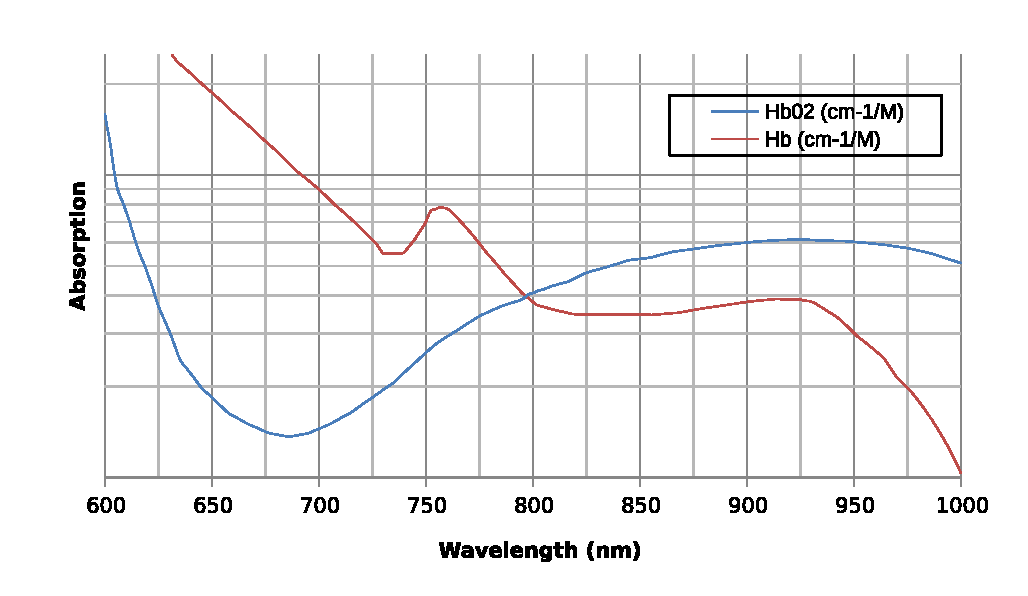
\includegraphics[scale=1,width=0.9\textwidth]{Images/hemoglobin.pdf} 
		\caption{Absorption Spectra of HbO2 (dashed) vs. Hb (Solid) }
	\end{center}
\end{figure}

For a single transmittance, measurement of a single light wavelength the resulting value depends on several factors. First, the reading will fluctuate based on the amount of tissue the light must pass through. However, the amount, and density, of tissue varies with time. To further accentuate the problem, the most important component of the signal accounts for only 2\% of the magnitude of the signal. Front end processing usually removes the non-pulsatile part of the waveform leaving only the pulsating part, called a plethysmograph. The resulting graph shows only the time varying signal, allowing for larger magnification of features [31].

One goal we have is an integrated smart patch located in one area of the body. The optimal location for measuring ECG is over the heart, while for O$_2$ Saturation the optimum location for a transmitve sensor is a finger or earlobe. Reflectance sensors do not have such limitations. Part of our research is to determine alternate sites for PPG measurement with a reflective sensor near the heart that provides adequate resolution.

\subsection{Accelerometers}
\label{subsec:Accelerometers}
An accelerometer is a small device capable of measuring changes in acceleration. In recent years, cost and size of these devices have resulted in Micro Electro-Mechanical Systems (MEMs) devices capable of measuring the acceleration an object is undergoing. Previous group research has shown it is possible to use acceleration data to augment our classifier algorithms to adjust for changes in motion \cite{Shannon2012}.  Outside research has also presented methods for on body device localization \cite{Vahdatpour2011}. 

Part of our proposed research is to integrate acceleration data into our calculations for our metrics. Combating noise  and motion artifacts is a prime concern since, in the research, clean waveforms for ECG and PPG are required to provide meaningful data.

While some methods focus on noise removals through activity-unaware means such as wavelet transforms \cite{Liu2011} we propose using the accelerometer data in two ways. First, minimally, the acceleration data can provide a confidence level to our acquired waveforms. In a binary movement analysis, where the result is either “moving” or “not moving”, we can choose to accept or discard our readings. With a more fine tuned approach, we can begin to associate movement with correlated changes in the ECG and PPG waveforms. Ultimately, we hope to use the accelerometer data to filter waveforms even in the event of extreme movement such as running. Second, the accelerometer data can be processed to determine the current level of patient activity and feed into our classifier algorithms. By providing and activity metric, our classifiers become more accurate. For instance, a 27-year-old healthy individual may have a normal heart rate of 63 BPM. Feeding a reading of 120 BPM into the classifier for such an individual could indicate some type of tachycardia. However if we add the processed accelerometer data showing the individual is stepping at 2.5 Hz, indicating a fast run, we can adjust our classifier to conclude that heart rates of 116 to 164 BPM could be considered normal.

\section{Data/Sensor Fusion}
\label{sec:DataFusion}
Thus far, the three primary sensors have been discussed separately. However, when information from all sensors is combined intelligently additional useful data can be derived than if only one sensor is available.  Combining sensor data intelligently is referred to as Data Fusion. Data Fusion can be defined as combining data from multiple sensors, and related information from associated databases, to achieve improved accuracy and more specific inferences than could be achieved by the use of a single sensor alone \cite{Hall1997}.  “Data fusion”, “Sensor fusion”,  ”multi-sensor fusion”, and “information fusion” have been used in the literature interchangeably \cite{Crowley1993} \cite{Ceruti2006} \cite{Dantu2006} \cite{Dong2006} \cite{Durrant-Whyte2005} \cite{Qi2001} \cite{Stanley2007} \cite{Wu2002}. For the rest of the dissertation the term data fusion will be used since not all of our data comes from sensors, as in the case of the DASI, MLHF, and HFSA questionnaires.  Some challenges of data fusion stem from the types and rates of data collected from dissimilar sensor types having different resolutions and accuracy \cite{Wu2002}.  Stanley discusses three distinct levels of data fusion: Raw Sensor data fusion (RSDF), Feature Level Data Fusion (FLDF), and Decision level data Fusion (DLDF) \cite{Stanley2007}.  

Raw Sensor Data Fusion is defined as multiple sensors measuring the same physical phenomenon. All the real sensors discussed (Accelerometer, ECG, and PPG) are observing and measuring the activity or movement of the patient and their heart. By using RSDF, additional data about the activity of the heart can be derived. RSDF is the core of our synthetic sensor concept and is applied to gain information about the patient's blood pressure (BP), heart rate (HR) and respiratory rate. RSDF is performed at the hardware level as sensor data is recorded. Each of the physical sensors can be evaluated on a beat-by-beat basis, to determine the physical phenomenon being observed. The Blood pressure (systolic and diastolic) is derived, on a single beat of the heart \cite{Poon2005}. The heart rate is simply a function of the time between beats, the R-R interval converted to beats per minute (HR=1/T$_{R-R}$). Oxygen Saturation is derived as a ratio of the Oxygenated versus the deoxygenated blood pumped to the body per heartbeat. The patient's respiration is a derived of the baseline drift of the ECG waveform. 

Feature level Data Fusion is defined as descriptive features extracted from multiple sensors measuring similar or dissimilar physical phenomenon, combined into a single feature vector,  processed using pattern recognition methods \cite{DaSilva2012}. WHIPPED takes full advantage of FLDF to derive more meaning from the raw sensors and synthetic sensors. Some analysis takes place at the hardware level with the rest performed on the mobile device level due to its higher processing power. Previous work has been done to create discretized and classify our sensors measurements \cite{Chaiyasucheeva2012} \cite{DaSilva2012}. Different classifications for the ECG waveform are extracted based on the timing of the principally important points (PIPS).  The waveform is then classified as Normal, Slow-fast heart rate, irregular rhythm, P wave abnormality, QRS Complex abnormality, and both P and Q wave abnormality. 

Traditional methods of detecting cardiac abnormalities rely on a “clean” waveform, one with very little noise. However, with ambulatory and mobile home-care out patients using a long term monitoring device movement artifacts ,such as signal noise due to patient movement, are not only likely, they are to be expected. Furthermore, one of the most common things a patient can do to improve their wellness is perform regular exercise, presenting an additional complexity to the reading and interpreting the ECG waveform. One of our classifications for an ECG waveform is “slow-fast heart rate” which can indicate a bradycardia (slow rate) or a tachycardia (fast rate). However, if a patient is exercising, a “fast heart rate” classification is not accurate. The rate may be faster than the patient's resting HR, but it is a normal HR for a patient who is exercising; and should therefore be classified as normal. Fusing the data from the accelerometer and ECG can solve both issues. Research has shown techniques to compensate the ECG signal for movement artifacts using an accelerometer. Furthermore, by classifying the movement types of a patient the bounds for “normal” heart rate can be adjusted \cite{Shannon2012}.

Decision Level Fusion, defined as fusion of sensor information using preliminary decisions/assessments for individual sensors, lies at the heart of our patient wellness concept. Using all the data gathered from a patient not only can the current state of the patient be analyzed, but also the trend of the patient's wellness, given all the temporal data collected. Temporal analysis can be performed by the BKE based on the information received from mobile communication device. The server can then analyze the biometric readings and validate them by using the psychosocial questionnaires to infer additional meaning. Finally, by consulting the cardiac ontology and the patient's history or EHR, including any co-morbidities, the patients can be informed of their own wellness measurement and offer interventions on an as needed basis. 

We conclude, based on available literature, extracting knowledge from our sensor patch, psychosocial and symptom instruments, and medical ontology subset can generate a relevant wellness metric for patients. Using an integrated, wireless, mobile sensor patch affords the possibility of generating additional metrics such as respiration rate and blood pressure that would not be possible with individual sensors.

\begin{figure}
	\begin{center}
		\label{fig:HR69}
		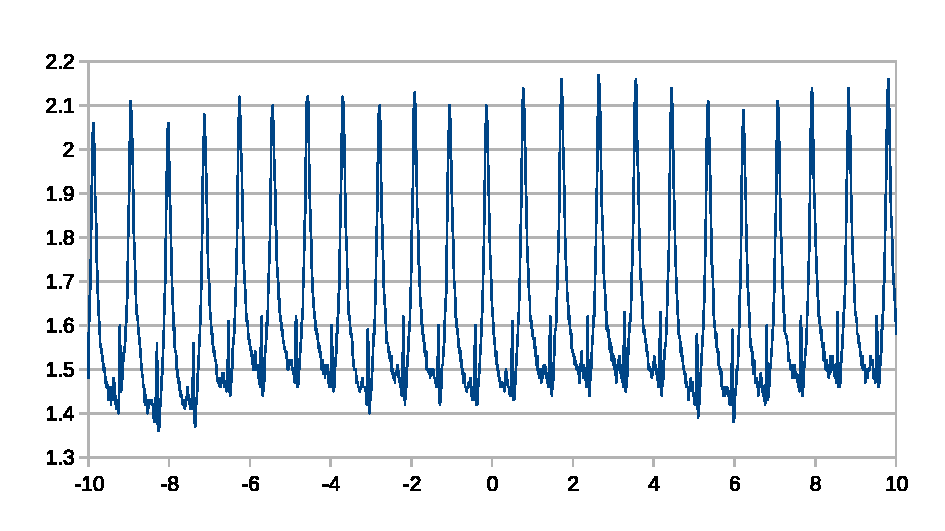
\includegraphics[scale=1,width=0.9\textwidth]{Images/HR69.pdf} 
		\caption{Sample Trace of ECG waveform with Heart Rate = 69}
	\end{center}
\end{figure}

\section{Synthetic Sensors}
\label{sec:SyntheticSensors}
By analyzing the two primary sensors, additional sensor data can be derived.  These derived measurements are called “synthetic sensors”. A synthetic sensor aggregates the data from other “real” sensors and calculates a measurement for a sensor type normally requiring additional hardware \cite{Fortier2009}. The synthetic sensor concept is illustrated in \cref{fig:SyntheticSensor}.

\begin{figure}
	\begin{center}
		\label{fig:SyntheticSensor}
		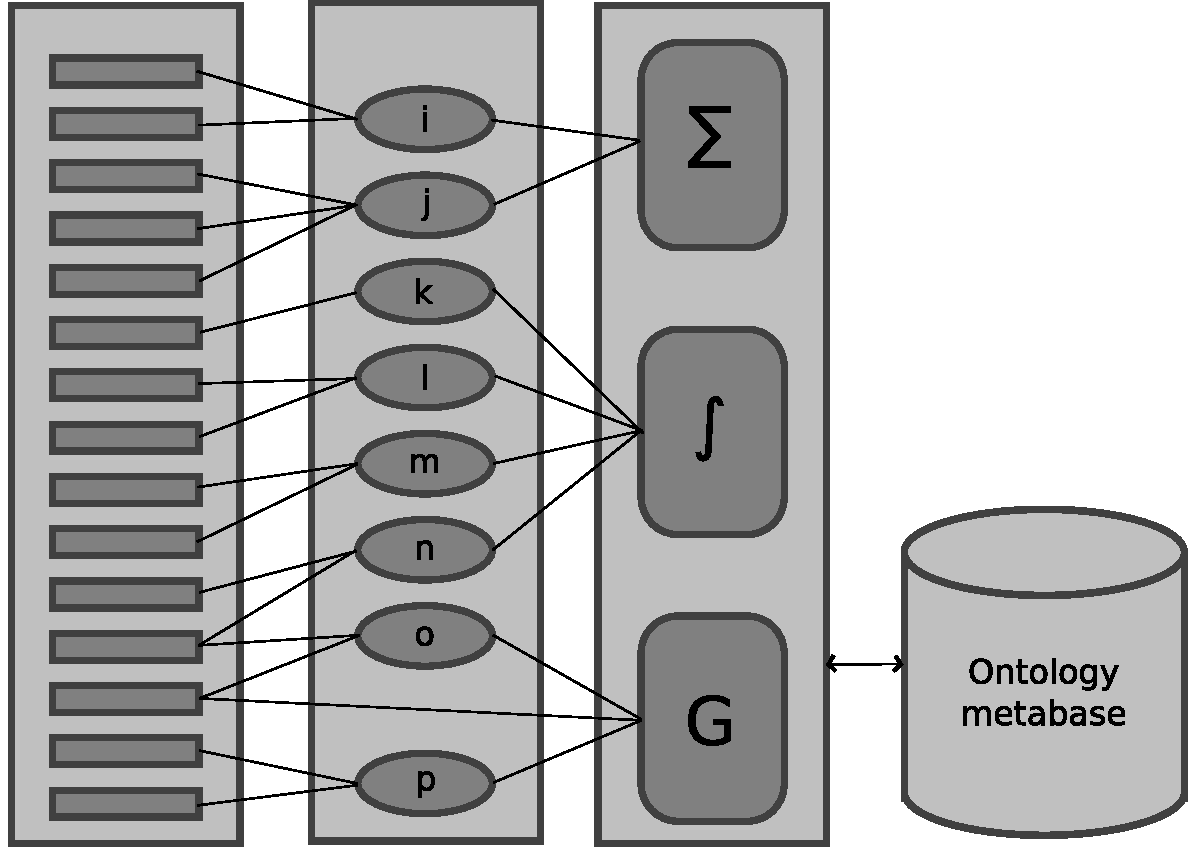
\includegraphics[scale=1,width=0.9\textwidth]{Images/syntheticSensor.pdf} 
		\caption{Synthetic Sensor Concepts for the Medical Domain}
	\end{center}
\end{figure}

\subsection{Pulse Rate}
\label{subsec:PulseRate}
The first and simplest synthetic sensor to construct, given our real sensors, is a pulse rate sensor. To derive the pulse rate a combination of signal processing techniques are used to identify the QRS complex of an ECG signal \cite{Chaitanya2011}. The number of QRS complexes per minute is the derived measurement of pulse rate, in beats per minute \cite{Scully2012}. Examining \cref{fig:20SecondEcg} shows a twenty-second ECG trace. \cref{fig:PulseRateCalc} shows the calculations necessary to determine heart rate.
\begin{figure}
	\begin{center}
		\label{fig:PulseRateCalc}
		$\frac{23 R-waves}{20 seconds}*\frac{60 seconds}{1 minute}=69 \frac{beats}{minute}$
		\caption{Basic Pulse rate calculation}
	\end{center}
\end{figure}

However, it is also possible to calculate the pulse rate on the R-R interval as shown in \cref{fig:RR_PulseRateCalc}. Calculating the heart rate in this way can produce fluctuations and a moving average based on the R-R interval can provide a more stable result.

\begin{figure}
	\begin{center}
		\label{fig:RR_PulseRateCalc}
		$\frac{1 beat}{T_{R-R} seconds}*\frac{60 seconds}{1 minute}=\frac{beats}{minute}$
		\caption{Heart Rate calculation from R-R interval}
	\end{center}
\end{figure}

The heart rate of a patient can be a primary indicator of heart health. If a patient's heart rate is elevated, barring other factors discussed in \nameref{sec:DataFusion}, it can be an indication of tachycardia. The heart rate is a principal input into the wellness metric calculation.

\subsection{Blood pressure}
\label{subsec:BloodPressure}
\begin{figure}
	\begin{center}
		\label{fig:BP_cuff}
		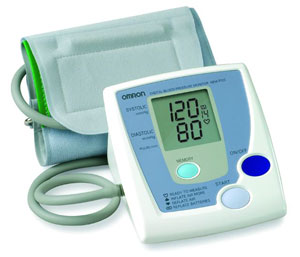
\includegraphics[scale=1,width=0.9\textwidth]{Images/BPCuff.png} 
		\caption{Commercially available blood pressure meter with auto-inflating cuff}
	\end{center}
\end{figure}

Blood pressure (BP) is a measure of the pressure exerted on the walls of the blood vessels, divided into systolic and diastolic pressures. BP is normally measured using an inflatable cuff (\cref{fig:BP_cuff}). The highest pressure occurs when blood travels through the arterial circulation by the contraction of the heart,  known as the 'systolic' blood pressure (SBP), while the 'diastolic' blood pressure (DBP) measurement is taken when the heart relaxes between beats and the pressure in the arterial circulation falls to its lowest level \cite{NOORDIN2009}. 

\begin{figure}
	\begin{center}
		\label{fig:PTT_calc}
		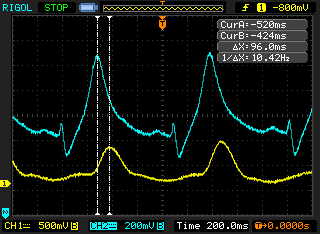
\includegraphics[scale=1,width=0.9\textwidth]{Images/PTT_Calculation.png} 
		\caption{Example calculation of Pulse Transit Time $ \Delta X $(PTT)}
	\end{center}
\end{figure}

Modern techniques for blood pressure calculation utilize a data fusion of the ECG waveform and the PPG to derive pulse wave velocity (PWV), inversely proportional to Pulse Transit time (PTT), to derive BP without the need for an inflatable cuff.  PTT is defined as the time between the detection of the pulse pressure wave in two locations on the body, usually the heart and the finger. Peak detection on the ECG and PPG trace result in two detection points (\cref{fig:PTT_calc}). Subtraction yields the PTT. In the figure, pulse transit times for the two heartbeats are 1.82-1.72=0.10 seconds and 2.76-2.64=0.12 seconds. Using such a synthetic sensor has several advantages, most notably a reduced impact on the user and no moving parts. Additionally, taking BP readings with a cuff can only be performed intermittently \cite{DeMey1995}. New non-invasive techniques allow BP to be recorded for each heartbeat allowing for continuous BP monitoring \cite{Gesche2012}. 

Calculating mean BP requires a per user calibration. During the patient's hospitalization, their blood pressure will be monitored. Each time a BP reading is taken the PTT will also be recorded. A regression can be performed since research has shown that PTT is highly correlated to BP \cite{Chan2001}. Once discharged, the calculated regression will be stored in the patient's WHIPPED system. For each heart beat the patient's BP can now be estimated.  

Further research has shown how to calculate SBP and DBP from a calibration measurement \cite{Poon2005}. A single measurement of a patient's PTT and a corresponding measurement of the patient's SBP and DBP are collected under clinicians care. Further BP readings can be collected every time a PTT is calculated using the formulas shown in \cref{fig:BPCalc}.\cite{Poon2005} Poon's method simplifies the application of the WHIPPED system.

\begin{figure}
	\begin{center}

		\label{fig:BPCalc}
		
		$DBP=\frac{1}{3}*SBP_{0} + \frac{2}{3}DBP_{0} + A*ln(\frac{PTT_{w_{0}}}{PTT_{w}})l-\frac{SBP_{0} - DBP_{0}}{3}*\frac{{PTT_{w_{0}}}^{2}}{{PTT_{w}}^{2}}$
		
		$SBP=DBP+(SBP_{0}-DBP_{0})*\frac{{PTT_{w_{0}}}^2}{{PTT_{w}}^2}$
		\caption{Blood pressure calculations, given pulse transit time }
	\end{center}
\end{figure}

For our research, we choose a cuff-less measurement algorithm, since it more closely matches our SWaP-C system goals. We will use a PTT method to eliminate the need for additional physical sensors while still achieving acceptable results. As an added benefit, we can monitor BP for every heartbeat without disrupting blood flow. Monitoring BP is important for patient health since high BP can cause harm to the body's blood vessels.

\subsection{Respiration Rate}
\label{subsec:RespirationRate}

Respiration is the number of breaths you take per minute. Traditional techniques in a hospital environment attached a strap across a patient's chest and based on the amount the strap was stretched the respiration rate could be calculated as the number of stretches per minute. Finding a way to derive the respiration rate with the need to attach a chest strap to a patient is necessary, since a chest strap is undesirable for the same reason an inflatable cuff is undesirable (SWaP-C). Modern hospital devices can derive the respiration rate from an ECG or PPG trace. Numerous methods have been documented such as the R-S Amplitude modulation method \cite{Dziuda2011} \cite{Noor2011} and the baseline wander method \cite{Scully2012} \cite{Ponomarenko2005} to derive the respiration signal from the ECG. A simpler band pass filter on the PPG waveform has also been used \cite{Scalise2011}. Scalise's approach has been augmented by adjusting the band pass filter based on the calculated heart rate \cite{Mason2002}.

Our literature review demonstrates that additional hardware is not needed to measure the respiration waveform of a patient. It is important to monitor respiration for CHF patients, especially in conjunction with Oxygen saturation. We seek to identify such events as apneas, and hyperventilation, and, using accelerometer data, aid in determining patient motion.

\chapter{Trial Results} 
\label{chap:trialResults}
%in this section i will first discuss the raw results of the trial, then discuss both the primary results (the raw data) and the secondary results (lessons on how the trial was run)

\section {Limitations of Trial}
The scope of the exploratory trial was limited after the Dissertation proposal due to timing of applicable grants. Some parts of the proposed design, including detection of PIPs, generation of targeted interventions, and wireless data delivery were reduced as a result, in scale in order to comply with the timing demands enforced by the supporting grants. The project was refocused on collecting physiologic and psychosocial data and post processing that data. The BKE was scrapped as a live updating entity, eliminating the requirement for a medical ontology.

The goal of the trial, was now to build and implement a system for data collection consisting of a non-intrusive sensor apparatus to collect psychometric data and a cellphone application to accumulate psychosocial data. The sensor would need to have its data manually downloaded each week by a visiting clinician. Detailed information about the sensor package can be found in \cref{chap:ProtoTypeBuildTest} : \nameref{chap:ProtoTypeBuildTest} .


\section{Exploratory Trial Initial Description}

Sethares et al. proposed a trial to assess the usefulness of the sensor design concepts including both the new sensor hardware and the cellphone application to collect somatic awareness data.  The trial was originally proposed to run from November 2013 through August 2014 \cite{KristenASethares2013}. Due to issues unrelated to research the first patient was not equipped with sensors until May 2014.

\begin{figure}
 \begin{center}
  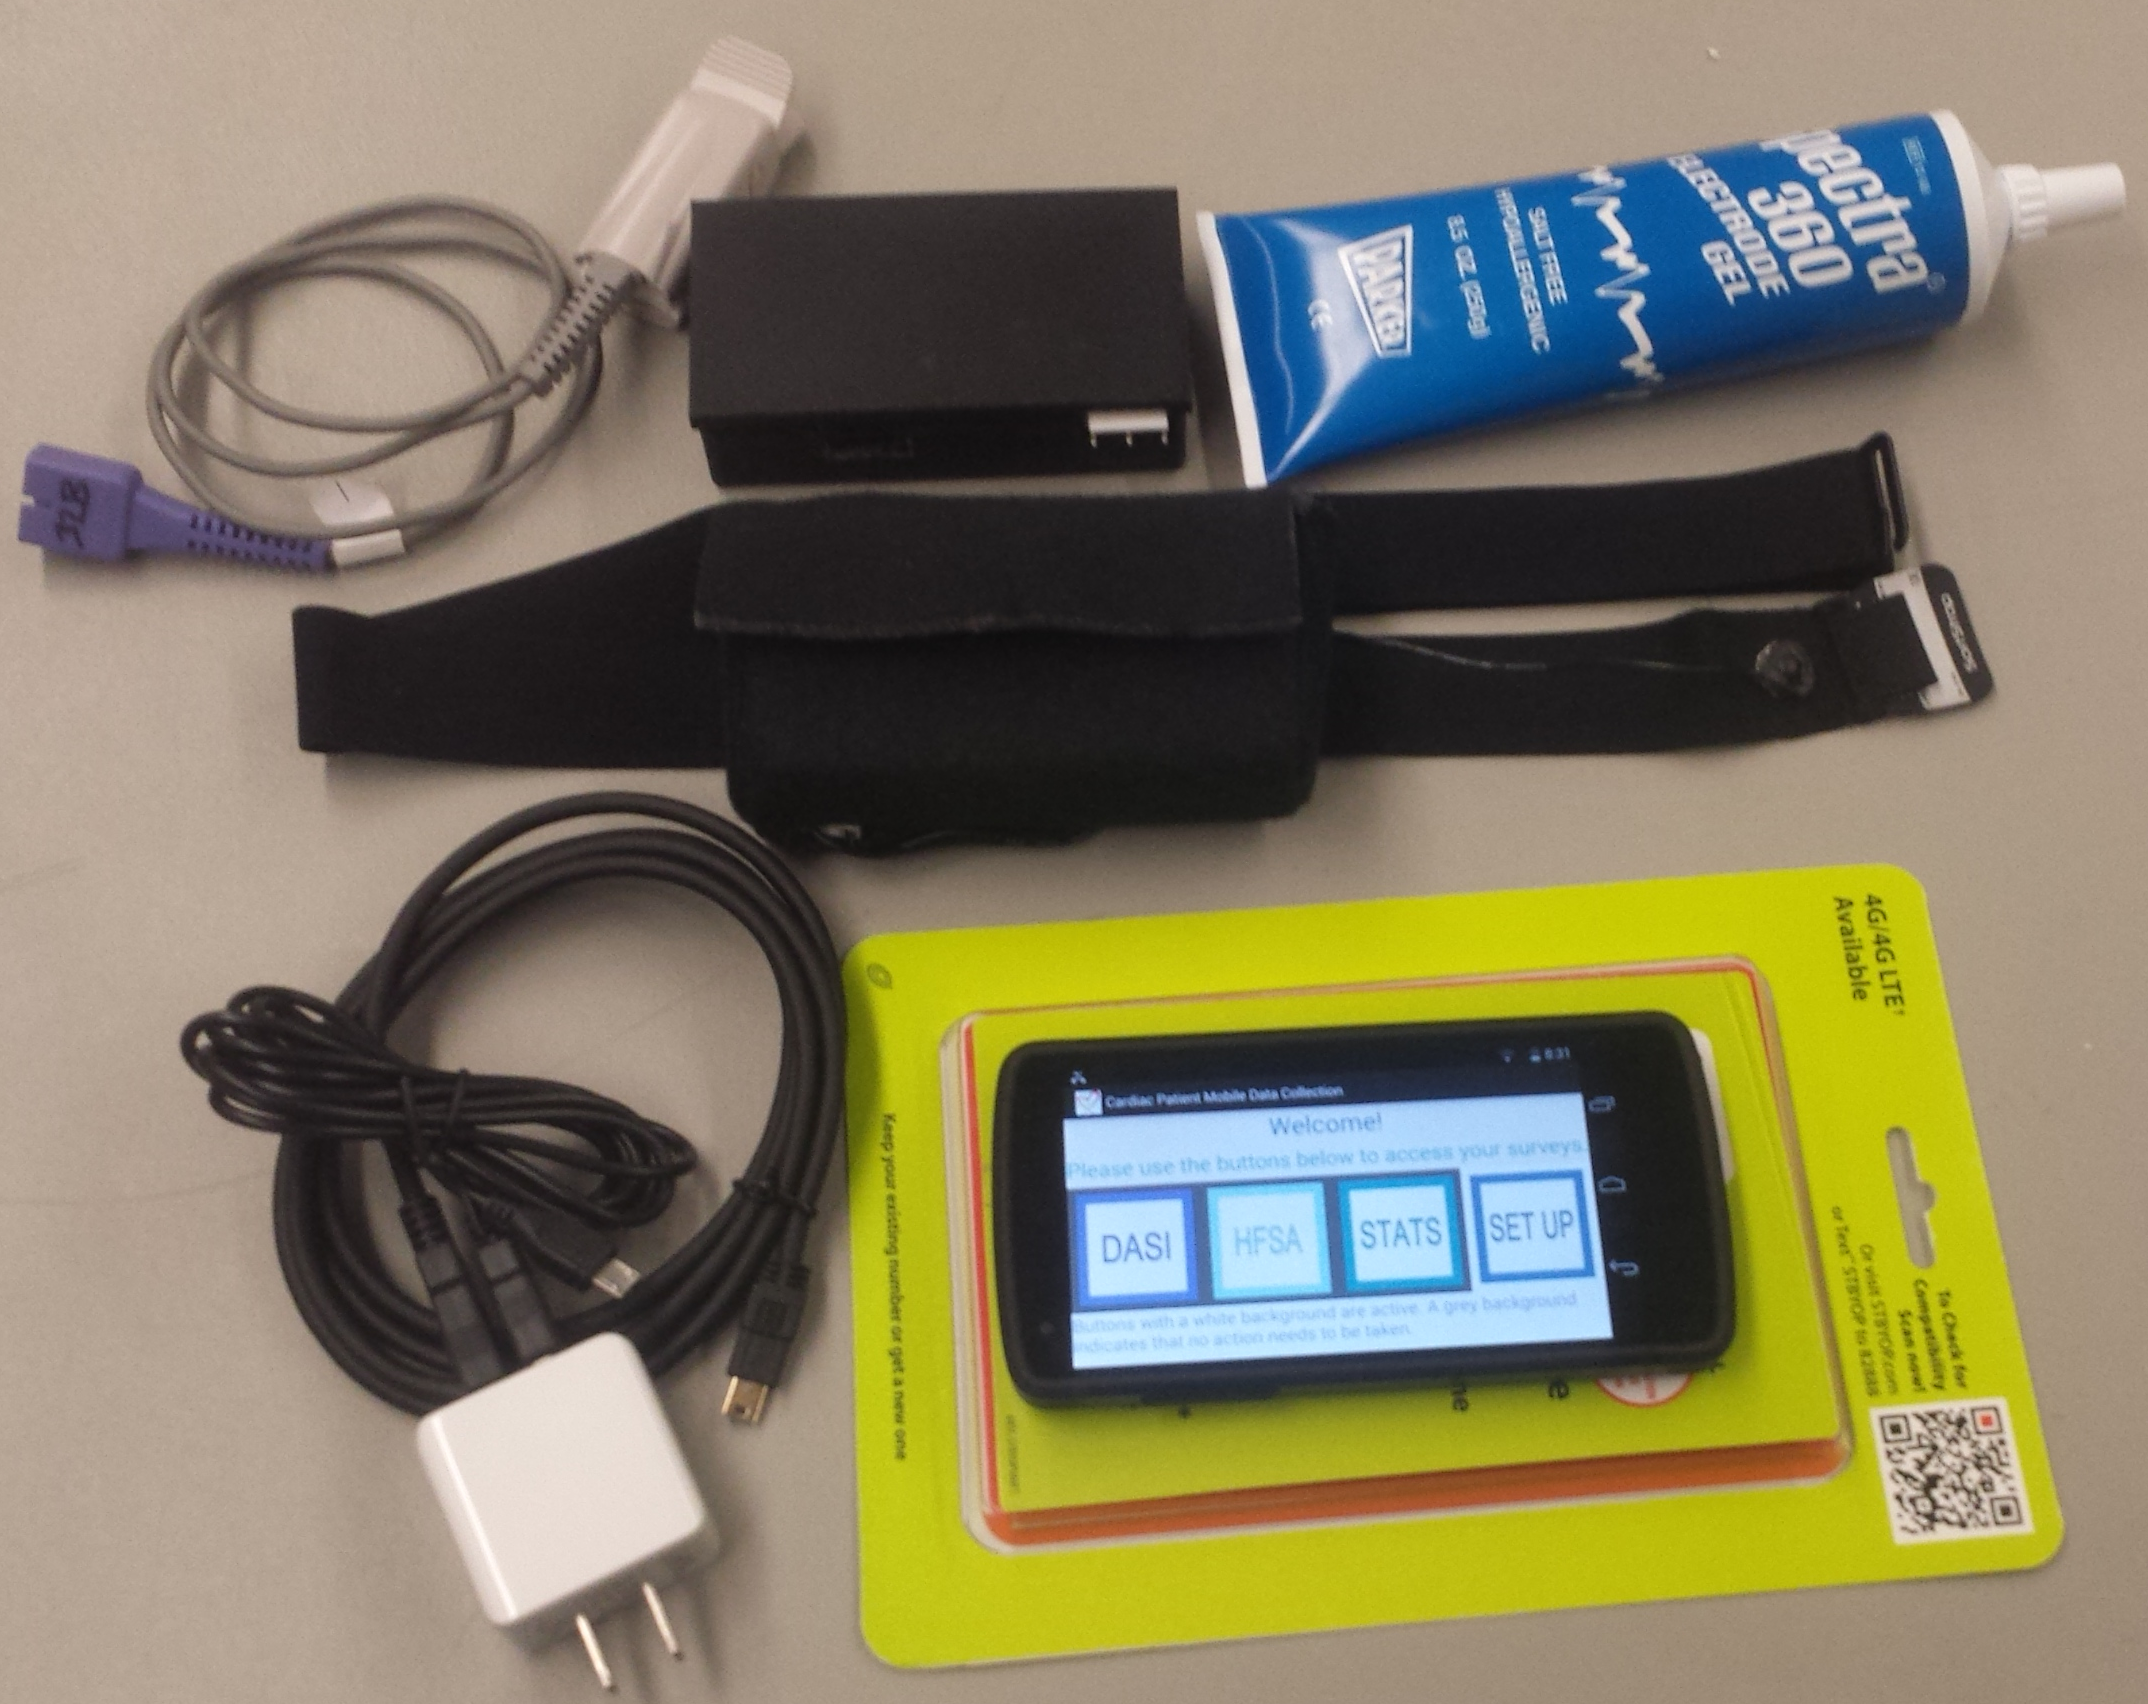
\includegraphics[scale=1,width=0.75\textwidth]{Images/carePackage.png} 
  \caption{Care Package for each Participant.} 
  \label{fig:CarePackage}
 \end{center}
\end{figure}



Each participant was provided with a package as shown in \cref{fig:CarePackage}:
\begin{itemize}
\item An lg nexus 5 cellphone with the heart monitor application
\item a sensor assembly
	\begin{itemize}
	\item a 3d printed enclosure
	\item a sensor board
	\item a modified polar(r) brand chest strap
	\item a fabric pouch
	\end{itemize}
\item a tube of electrode gel
\item a two port USB charger
\item a USB A to USB mini cable
\item a USB A to USB micro cable
\end{itemize}

The patient was instructed to wear the device during the day and to wear the finger clip, when convenient. The patient was instructed to take off the device and plug it in to charge at night . Additionally, the patient was given a smartphone, with a data plan, and shown how to use the survey application (app). 

\begin{figure}
 \begin{center}
  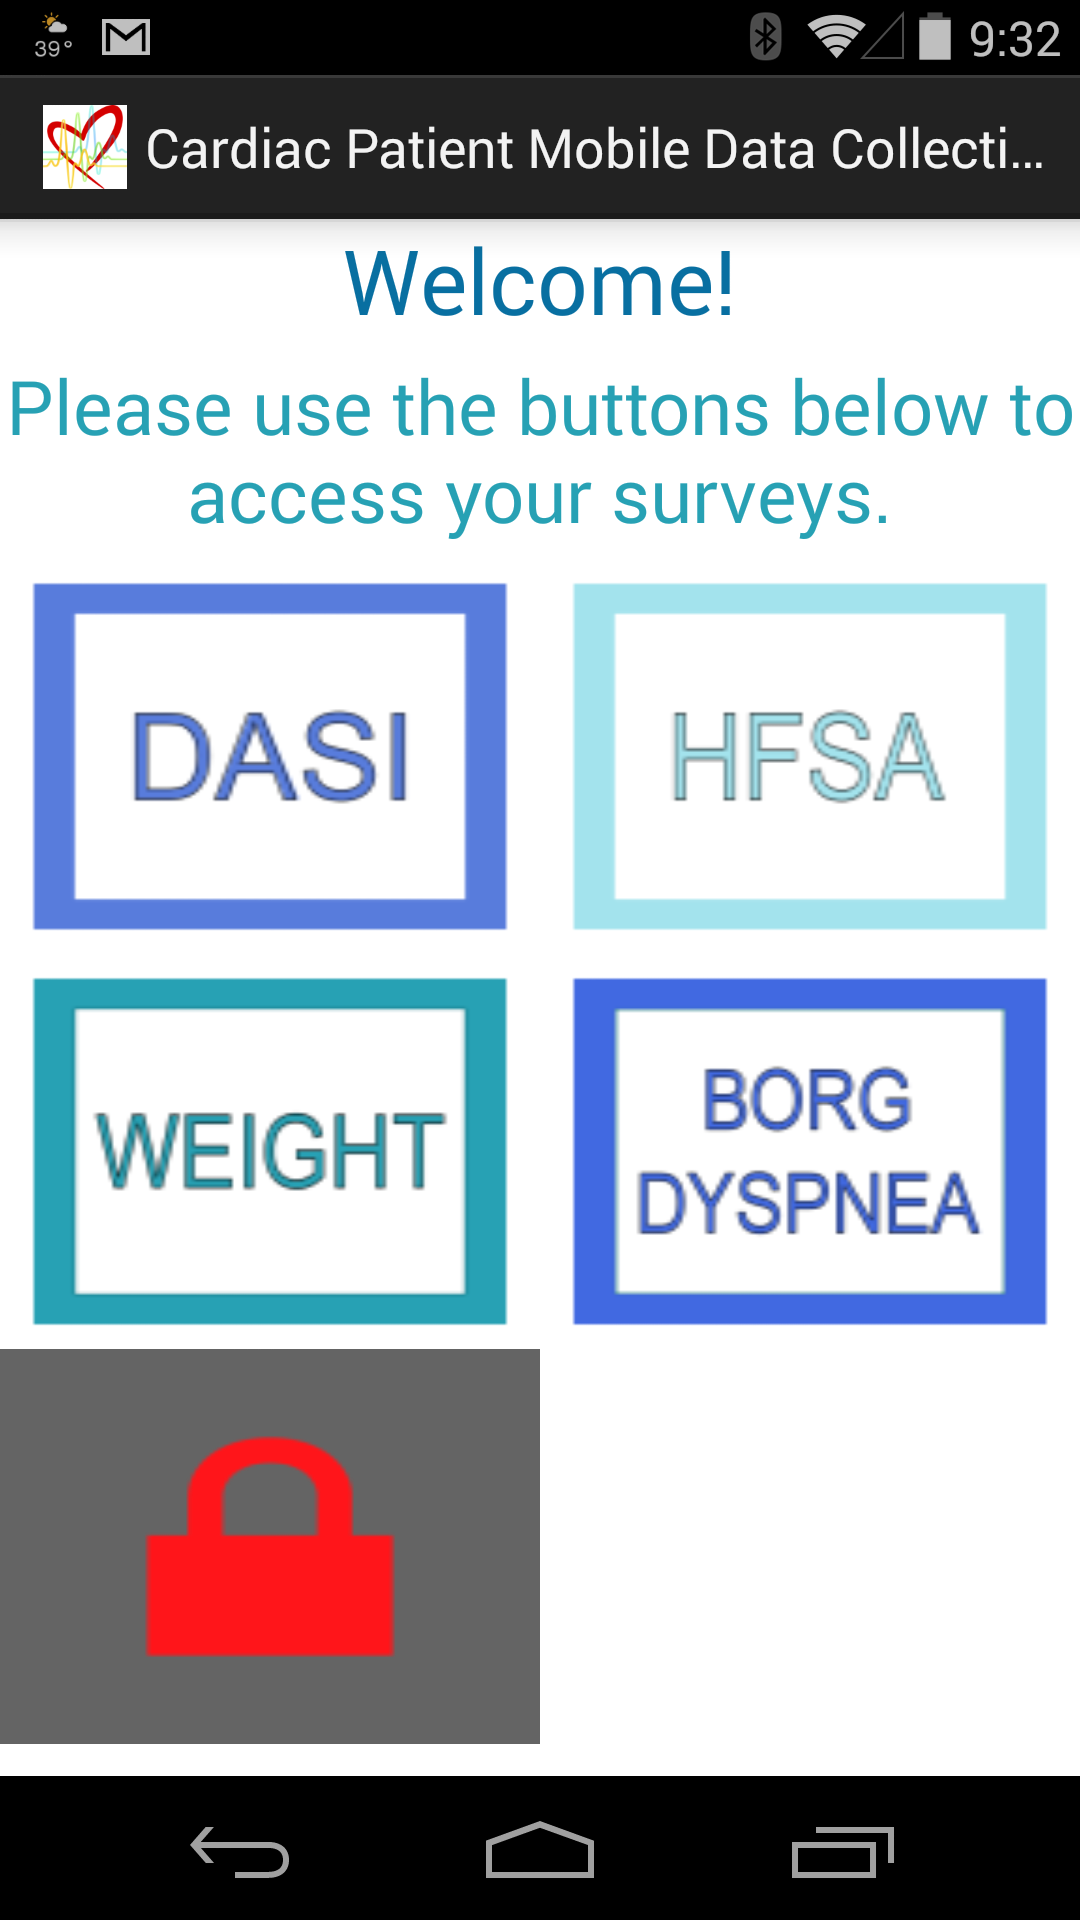
\includegraphics[scale=1,width=0.3\textwidth]{Images/AndroidSplash.png} 
  \caption{Main Screen for Smartphone Apps} 
  \label{fig:AndroidSplash}
 \end{center}
\end{figure}

\section{The Phone Application}

The smartphone application was written in Java by an undergraduate researcher, based on previous masters projects in the MCHM research group \cite{Louro2013,Putin2011}. The application underwent several revisions over the course of the trial. \cref{fig:AndroidSplash} shows the initial screen presented to enrolled patients when they started the app. allowing for weight and dispnea data entry or to trigger a psychosocial survey.

The first iteration implemented a different version of one of the psychosocial assessment tools, using a 1-4 lickert scale, the instrument was supposed to have 0-5 with 0 indicating ``I did not have that symptom''. It also did not have the self reporting behaviors for COPD patient. Last, there was no alarm feature implemented inside the survey application to remind the patients to participate in the self care instruments.

\begin{figure}[ht]
\centering
  
  \begin{subfigure}[b]{0.3\textwidth}
  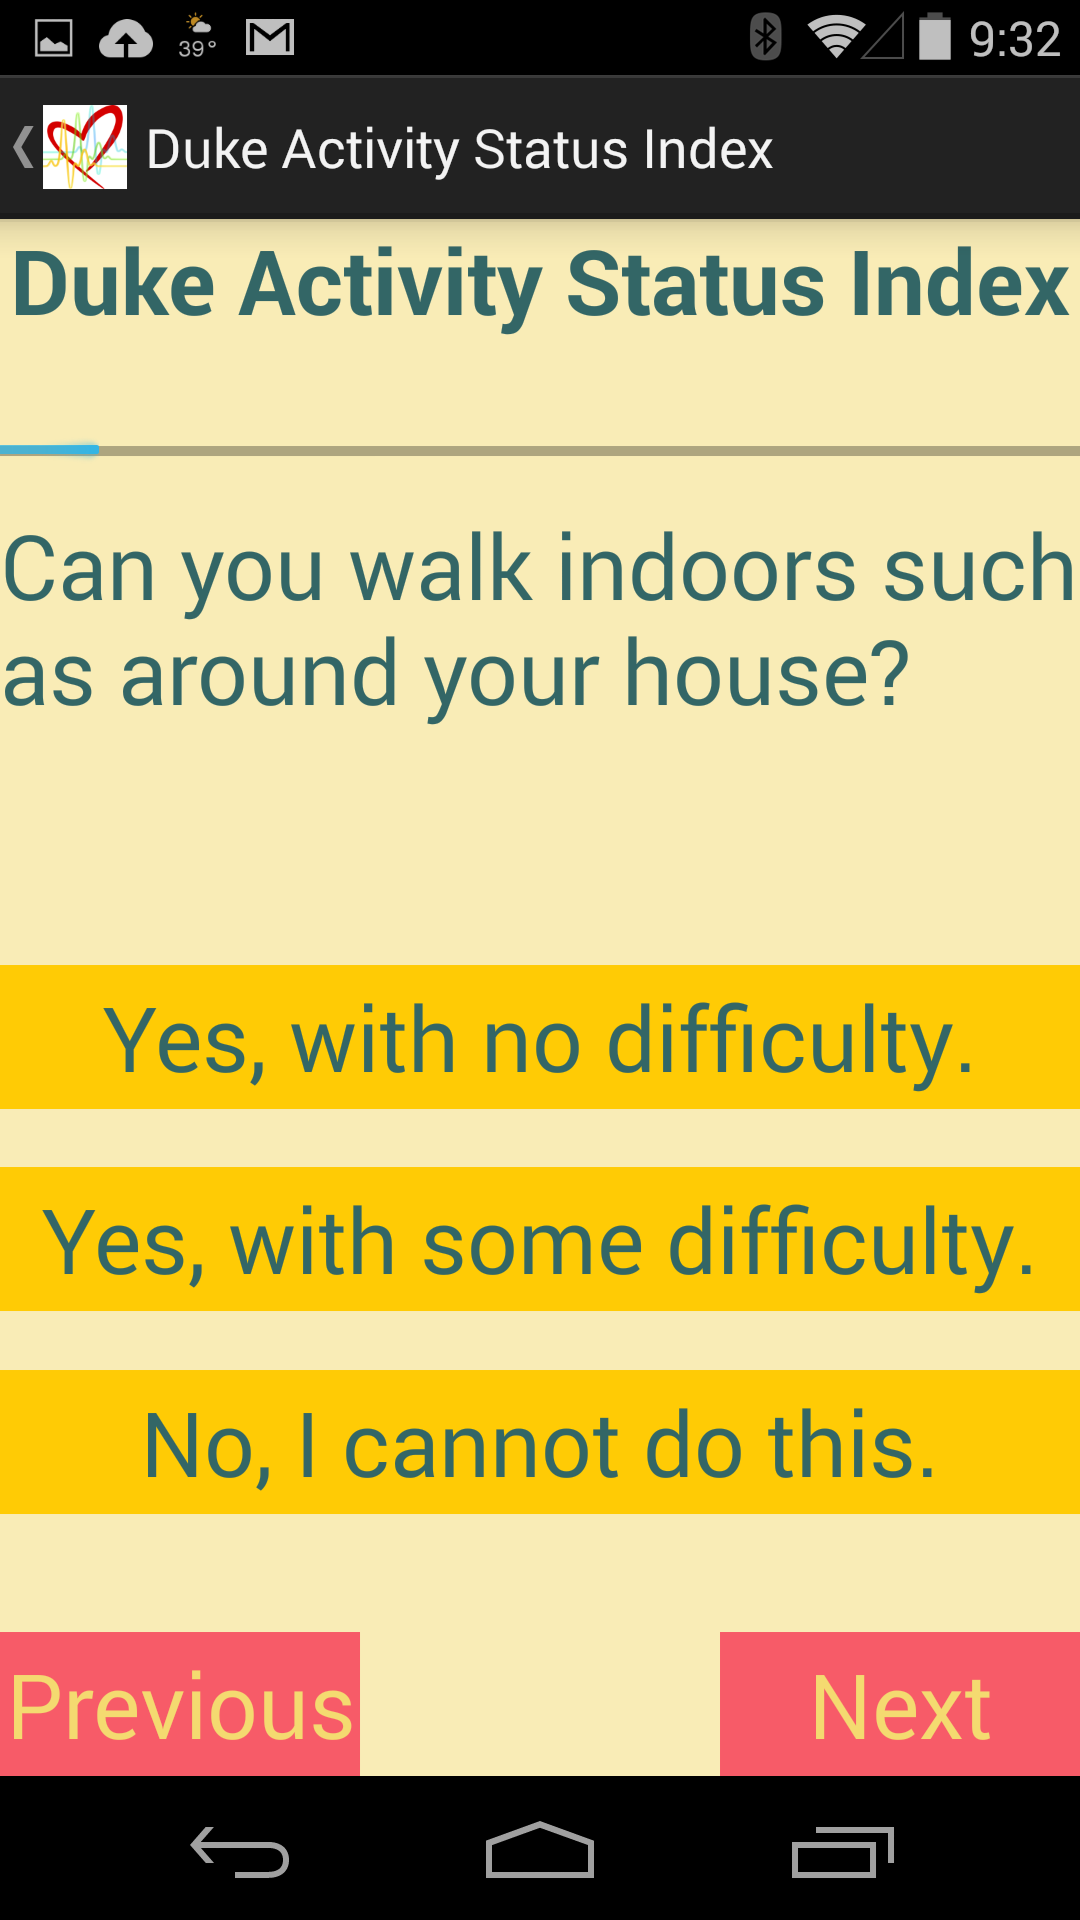
\includegraphics[scale=1,width=\textwidth]{Images/DASI.png}
  \caption{DASI Survey}
  \label{fig:DASI}
  \end{subfigure}
  ~
  \begin{subfigure}[b]{0.3\textwidth}
    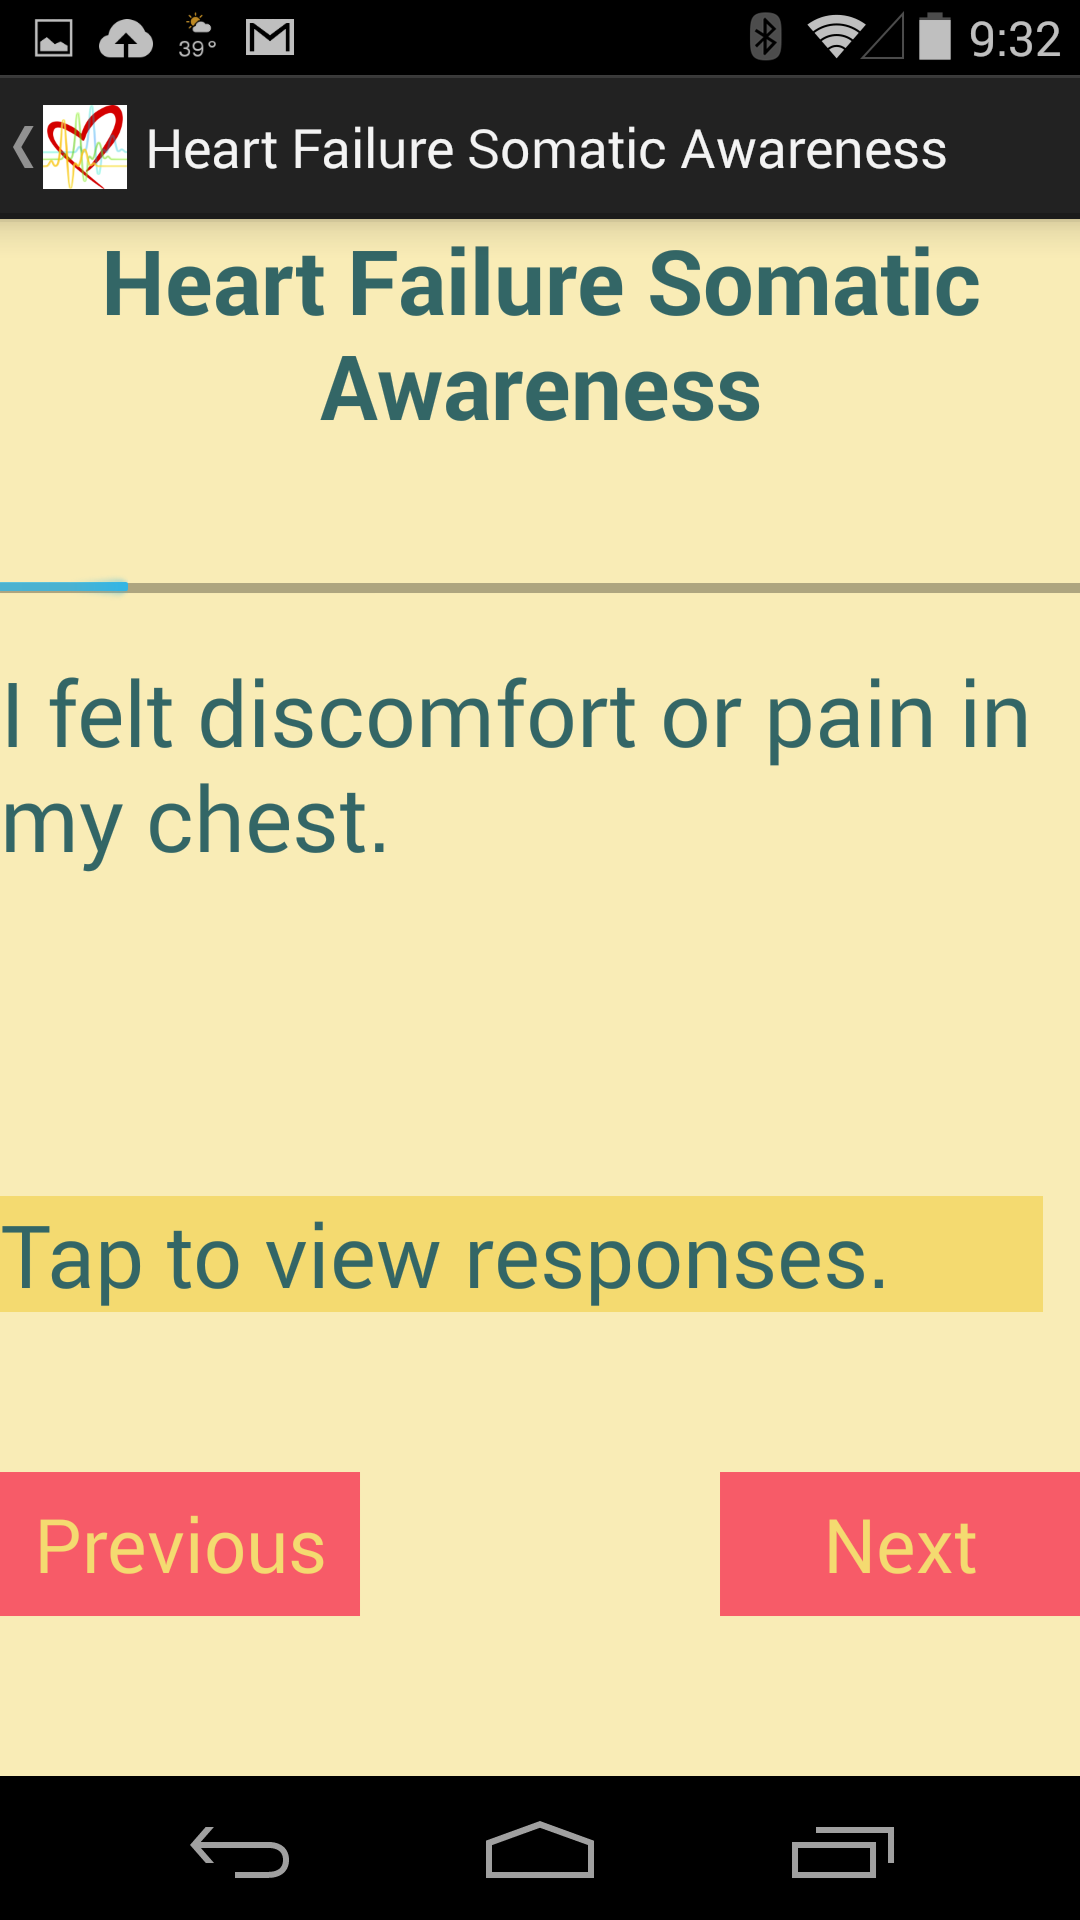
\includegraphics[scale=1,width=\textwidth]{Images/HFSA_question.png}
	\caption{HFSA Question}
  	\label{fig:HFSA_Q}
  \end{subfigure}
  ~
  \begin{subfigure}[b]{0.3\textwidth}
    	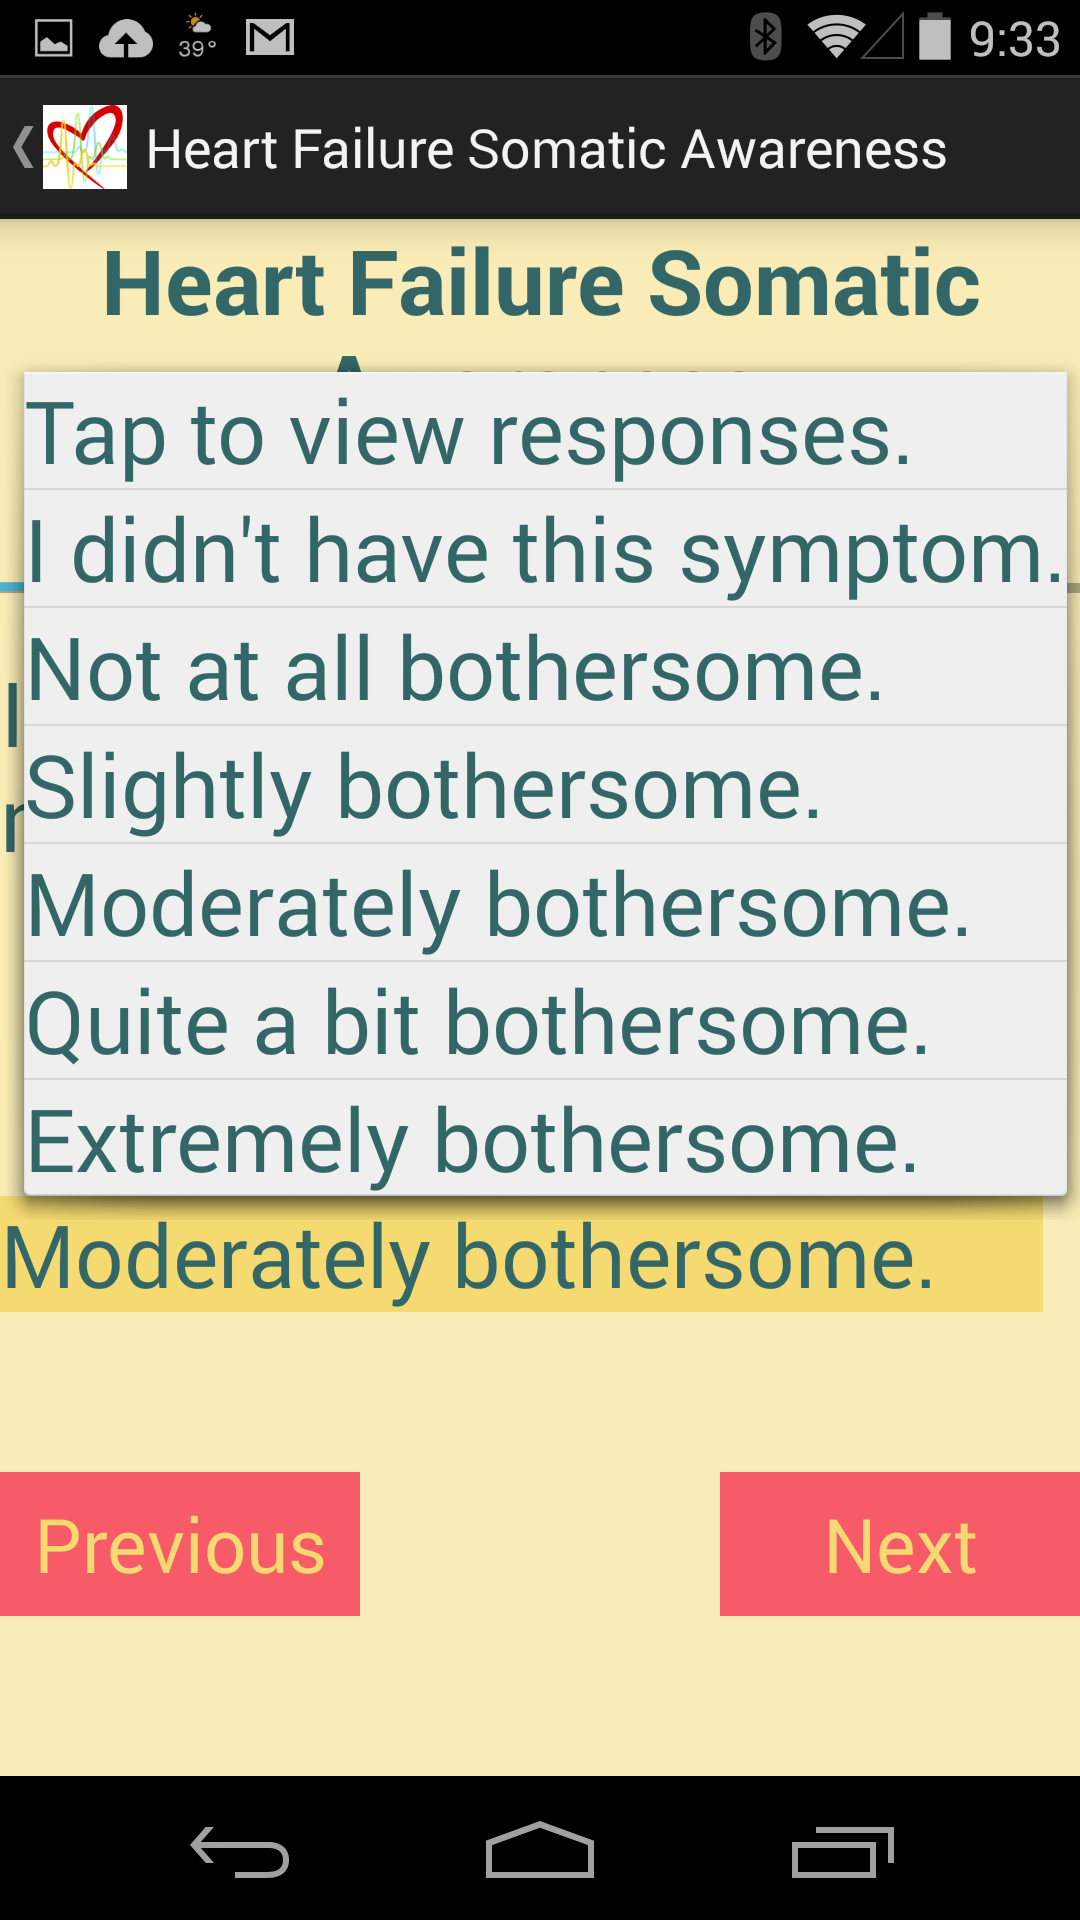
\includegraphics[scale=1,width=\textwidth]{Images/HFSA_answer.png}
  		\caption{HFSA Responses}
  		\label{fig:HFSA_R}
  \end{subfigure}
  \caption{Psychosocial Entry Screens} 
  \label{fig:AndroidSurveys}
\end{figure}

The timing of when the surveys should be administered was a reoccurring problem. Initially the phones clock alarm was used to remind the patients of when the surveys should be taken. This came to a sudden halt when one patient was unable to deactivate the alarm, only snooze it for 15 minutes at a time, for 3 days. The decision was made to remove the alarm feature from the protocol after this patient. Additionally, at the start of the trial, the patients were not allowed to take the survey instruments more than 3 times a week, as indicated by the initial proposal. However, the resulting user experience was suboptimal, the prevailing reaction to being unable to take a survey was the perception the patient had done something wrong, resulting in frustration. A modification was made to allow the surveys to be taken at any time.

Unfortunately, integrating the required fixes for the changed lickert scale introduced an error in the submission process for the HFSA instrument that went unnoticed for several months. It was ultimately fixed but the patient information was un recoverable.

Each survey was administered one question at a time, the different types of surveys each required a unique data entry technique as seen in \cref{fig:AndroidSurveys}. For the DASI, \cref{fig:DASI}, three buttons were available, pressing one, both chose the answer and advanced to the next question. For the HFSA, \cref{fig:HFSA_Q}, a dropdown box would be available to select an answer, \cref{fig:HFSA_R}, then the user would have to manually advance to the next question. 



\section{Trial Lessons Learned}

While the WHIP sensor system was the primary focus of the dissertation, the information gathered during the exploratory trial was just was important. Recording what went wrong is just as important as recording the primary data. The primary data collected was the biometric data, consisting of ECG and \spo2, and the psychosocial data, consisting of the DASI and HFSA instruments. 

\subsection{Lack of Time}
The largest obstacle present during the pre-study period, was time. Due to the urgency of the funding situation, several parts of the system were scaled back.  First, there was not time to integrate live result uploads into the WHIPPED system. Therefore, no back-end processing was performed on the real time data. Also, by not taking advantage of the wireless link between cellphone and WHIP sensor, the trial protocol was modified to include weekly visits to the patients to collect data on SD cards and replace them with empty cards. Additionally, the wireless link was supposed to allow for firmware updates of the WHIP sensor if needed. Removing the wireless link these features were deferred for the exploratory study.

In a traditional design cycle for a product, testing, or validation, may be the last step; but, it is the most important. Most designs go through several stages of testing. Alpha testing usually occurs in a lab setting where environmental factors are carefully controlled. Logical errors can usually be spotted and eliminated, in alpha testing. Beta testing widens the scope of tests, bringing the Device Under Test outside of the lab but controlling the population; limiting the population to participants who are familiar with the technology. Beta testing can be a much longer test procedure. However, to comply with the grant timing requirements. Both the device and the smart phone application were pushed into service without any beta testing. 

Another piece of the design which needed to be rushed was the wearable design. Using the polar heart strap was a decision born of expedience. It was faster to buy off the shelf straps and modify them to fit the needs of the grant. A less polished physical design was the result.

\subsection {Lost Data}
The primary goal of the WHIPPED system, after adjustments due to grant timing, was data collection. Several lessons were learned during the study. The sensor system was designed to record a theoretical maximum of eight-twelve-hour days. Originally, this was viewed as a comfortable margin of error since a nightly wireless data dump was envisioned at design time. Once the wireless link was removed from the study, a new protocol was put in place, data would be downloaded via the USB interface of the WHIP sensor. Someone would go to each participant each week with a computer and manually download the data.

The USB approach was quickly abandoned, due to speed. The USB hardware interface was only capable of full-speed USB (12 Megabits (Mb)/sec). Given that each 2 hour ECG and \spo2 datafile was approximately 100 MegaBytes (MB), one weeks worth of data would have taken $ 7 \frac{days}{week} * 8 \frac{hours}{day} * 100 \frac{MB}{2 hours} * 12 \frac{Mb}{Second} = 31.1 \frac{minutes}{week}$ to transfer data. In the future, if a microcontroller with a hi-speed USB interface is used, the same transfer would only take $ 7 \frac{days}{week} * 8 \frac{hours}{day} * 100 \frac{MB}{2 hours} * 480 \frac{Mb}{second} = 47 \frac{seconds}{week}$.  

Regardless of future implementations, the end result for the exploratory study, was that the SD cards were exchanged each week. 
Exchanging SD cards weekly led to a new set of problems. First, the one week limit on data storage was not explained to the study administrators, as a result, some patient data was lost when more than eight days elapsed between visits and the starting data was over written. This was later explained in more detail, and rectified, but the data was irretrievable. 

SD cards proved to be not able to handle the frequent handling and travel the exploratory study required. Two major sources of lost data involved the excess handling of sd cards and handling of the SD card to USB adapter used to download data from the sd card to a computer.

SD card readers require an external interface to transfer data to a computer. Several SD-to-USB converters were purchased for the purposes of the exploratory trial. At some point of during the trial one converter suffered a failure that went undiscovered for several weeks. Data files were transfered but files contained random data. When the same SD card was put into a different reader, the data was valid. To keep things as simple as possible the decision was made to no, longer use sd card adapters to download data, instead data cards would be exchanged for fresh cards and delivered for transfer where the data could be verified. This led to another problem related to the SD cards.

Like most electronic devices sd cards are sensitive to electro-static discharge (ESD). SD cards should be kept in a ESD-safe case when not inserted into a device. During the exploratory study, that was not always the case. 
As a result, entire sd cards worth of data were corrupted.

In future iterations, if wireless transfer is not available, the SD card protocol should be clearly documented. Additionally, a utility to visualize the data immediately after download would add a confidence factor for the study workers during home visits.


%\paragraph {too long between visits}
%\paragraph {bad SDcard adapter}
%\paragraph{excessive SD card handling}

\subsection{Lack of Documentation}
Lack of time had the additional effect of leaving no time for writing documentation for either the nursing faculty or the patients who would be using the device. All training was done in person. Future studies should have at least:
\begin{itemize}
\item a smartphone user manual.
\item a WHIP troubleshooting guide
\end{itemize}

A manual could take the form of written booklet, on-line video, or both. 
While the focus of the aforementioned items is on the patient and clinician, the need for manuals for engineers engaged in multidisciplinary work is even more acute. Specifically, when implementing the psychosocial instruments, great care was taken to ensure that data was validated before being inserted into the database. However, the sample space of possible answers was not made clear from the sample form provided. The one-to-five lickert scale could also contain responses such as ``does not apply'' or fractional values, such as ``0.5''. This lack of documentation resulted in many patches to the smartphone application, slowing down the trial. In the future it may be useful to have engineers that will be instrumenting similar psychosocial instruments follow on with clinician as they administer the surveys. If it is not possible to accompany clinicians, it may also be beneficial to collect a large dataset of filled in forms. Analysis of collected forms may also avoid confusion.

%\paragraph{cellphone user manual}
%\paragraph{WHIP troubleshooting guide}
%\paragraph{ digital surveys vs soft surveys}

%\subsection{Communication Problems}

%\subsubsection{patient - nurse communication}
%\paragraph{cellphone usage}
%\paragraph{proper strap placement/usage}

%\subsubsection{Feature creep}
%\paragraph{COPD - Borg Dispnea}
%\paragraph{modified likert}
%\paragraph{survey alarms}
%\paragraph{strict survey -> anytime survey}

%\subsubsection{nurse - engineer communication}
%\paragraph{delay between problem observation and problem reporting}
%\paragraph{no timely feedback on collected data}


%\subsection{Loose protocol adherence}
%\paragraph{ changes in survey protocol, database changes}
%\paragraph{ changes in sensor useage (finger clip)}
%\paragraph{ no calibration measurements}
%\paragraph{ ECG Disconnected}

\chapter{Prototype Construction and Testing}
\label{chap:ProtoTypeBuildTest}
%This chapter will detail the process of integrating the three parts of the WHIPPED system together to make an end-to-end application. I will first discuss integrating the smartphone and sensor suite to gather physiometric data. Then discuss the integration of the smartphone and BKE, separate from the sensors, to communicate psychosocial information. Finally, I will discuss the BKE‘s integration of all knowledge from both the sensors, via the smartphone, and the psychosocial data to calculate wellness and provide interventions.

%i apologize for the 62 times i use the word module.

This chapter covers the Hardware design and unit testing of the Wireless Health indicator patch (WHIP) and its initial construction. The different modules of the final prototype are outlined and their overall integration discussed, Procedures for testing the functionality of the design in a laboratory environment are discussed. Next, the physical design of the sensor apparatus is covered.

\section{Electronic Design}


The core of the dissertation is the Wireless Health Indicator Patch (WHIP). This device, if properly connected to a patient, records all the needed data to derive the metrics described in \nameref{chap:SensorConcepts} and stores this data to a Secure Digital (SD) card for later retrieval. Additional functionality is offered via a Bluetooth (BT) connection. The final device used for the trial is the fifth revision of designs dating back to 2011. Details on previous versions can be found in \nameref{sec:ResearchDoneToDate}. The remainder of this section focuses on the final prototype.

The WHIP device consists of several modules, interacting across a standard communication buses. Each device is discussed including the power-module, the Memory-module, the ECG-module, the \spo2-module, the Communication-module, and finally the control-module. Once each module is fully defined the methods for integration are covered. Many of the modules have evolved from the first prototype, starting as simple fixed modules and becoming more configurable at the expense of an increased component count and complexity. The final prototype consists of many modules with only a singe chip or device handling all the details of the module internally, as in the case of the ECG, \spo2, SD card, and Bluetooth modules. The important part of defining each module is to specify the inputs and outputs of each module as well as any protocols used to communicate with the device.

\subsection {The Schematic Capture}
The following sections discuss different modules that were synthesized for the Whip sensor. These schematics were created in Cadsoft eagleCAD (Eagle)\cite{Eagle2017} a schematic capture and layout program. Eagle was used to both layout the schematic and PCB. The full schematic is included in \cref{chap:PCB_Schematics}, however, figures for each module are included below.

\subsubsection {The Power Module}
\begin{figure}
	\begin{center}
		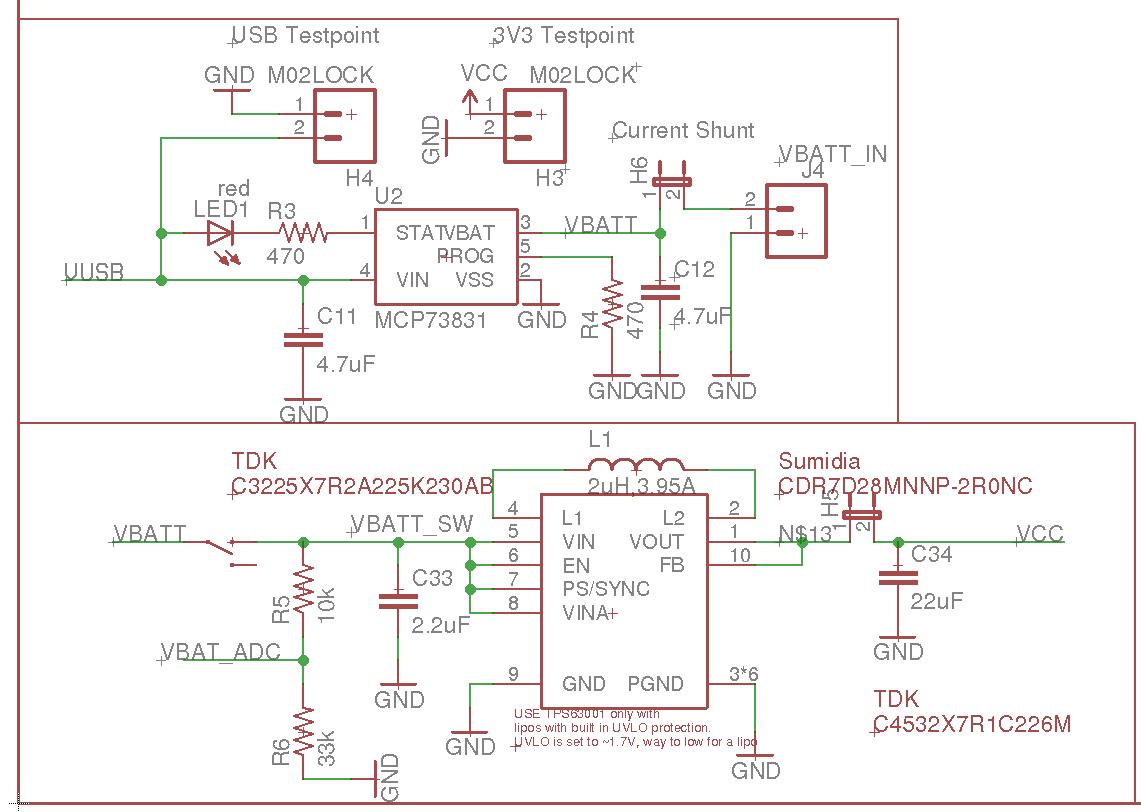
\includegraphics[scale=1,width=0.9\textwidth]{Images/Rev5_PowerSch.png} 
		\caption{Power Supply and Charging Circuit for Whip Sensor}
		\label{fig:Rev5_power}
	\end{center}
\end{figure}

\Cref{fig:Rev5_power} shows the schematic for the power module, responsible for providing power to all other modules. All modules are configured to operate at 3.3 Volts to simplify design. The other requirement for the power module is the ability to operate from, and charge, a single cell lithium polymer (LiPo) battery. Ultimately a design based on an existing open source power module was constructed \cite{Sparkfun2012}. Modifications to the Open Source HardWare(OSHW) design increased the current carrying capacity, and inflated the charging rate.

The power and charging design was featured on every WHIP prototype starting with version 1. The regulator circuit is based around the TPS61200 family of Buck/Boost regulators\cite{TPS610X}, this IC will provide a regulated 3.3V output over the entire range of a LiPo's voltage range, roughly 4.2 to 2.9 volts. Battery charging is handled by the MCP73831, a monolithic charge handler\cite{MCP73831}. The MCP73831 converts USB power, when available, to an appropriate charge voltage. The module uses a two pin keyed JST connector for connection to the battery and mini USB is used to provide power to charge the battery. Mini-USB was chosen over Micro-USB with the assumption that it would be easier for sight impaired users to correctly plug the device in. the power module also provides informational signals to the control module about battery health and charge status.

%JST doesnt stand for anything its the name of the company... %

\subsubsection {The Memory Module}
\begin{figure}
	\begin{center}
		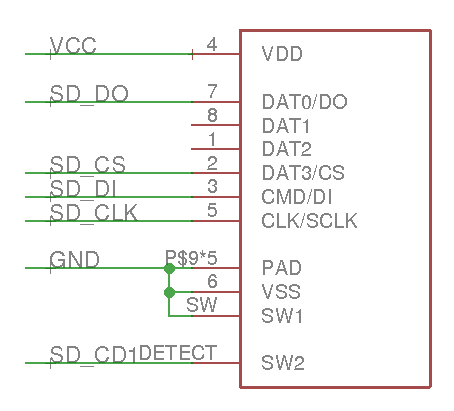
\includegraphics[scale=1,width=0.5\textwidth]{Images/Rev5_SDCARD.png} 
		\caption{Memory Circuit Connections for Whip Sensor}
		\label{fig:Rev5_SDCARD}
	\end{center}
\end{figure}
The Memory module is responsible for saving all patient biometric data. The device chosen was a micro SD card. The first revision of the WHIP board included a full sized SD card was as a trial of the technology. A micro SD card was used in the final prototype to reduce device size. The interface, shown in \cref{fig:Rev5_SDCARD}, remains the same regardless of card configuration. SD cards can communicate using the Serial Peripheral interface (SPI). SPI is a de facto standard, no standards body maintains the specification of SPI. SPI uses 4 wires to provide a full duplex synchronous communication channel. The memory module for the WHIP is actually the SD card, the only other part of the module is the card socket. All read and write logic is handled by the circuitry on the card. Offloading the flash algorithms to an sd card greatly simplifies the board design. However, SD cards are not 5 Volt tolerant this was part of the reason the power module provides 3.3V. The SPI bus for the memory module allows the control module to use a full FAT32 file system on the SD card using only the SPI interface.

In the Eagle the SD card device was created as a custom component and footprint. Then, to simplify the schematic diagrams off-page connectors were used to create a logical connection to the processor unit without cluttering the system diagram with excessive net wires.

\subsubsection{The ECG Module}
\begin{figure}
	\begin{center}
		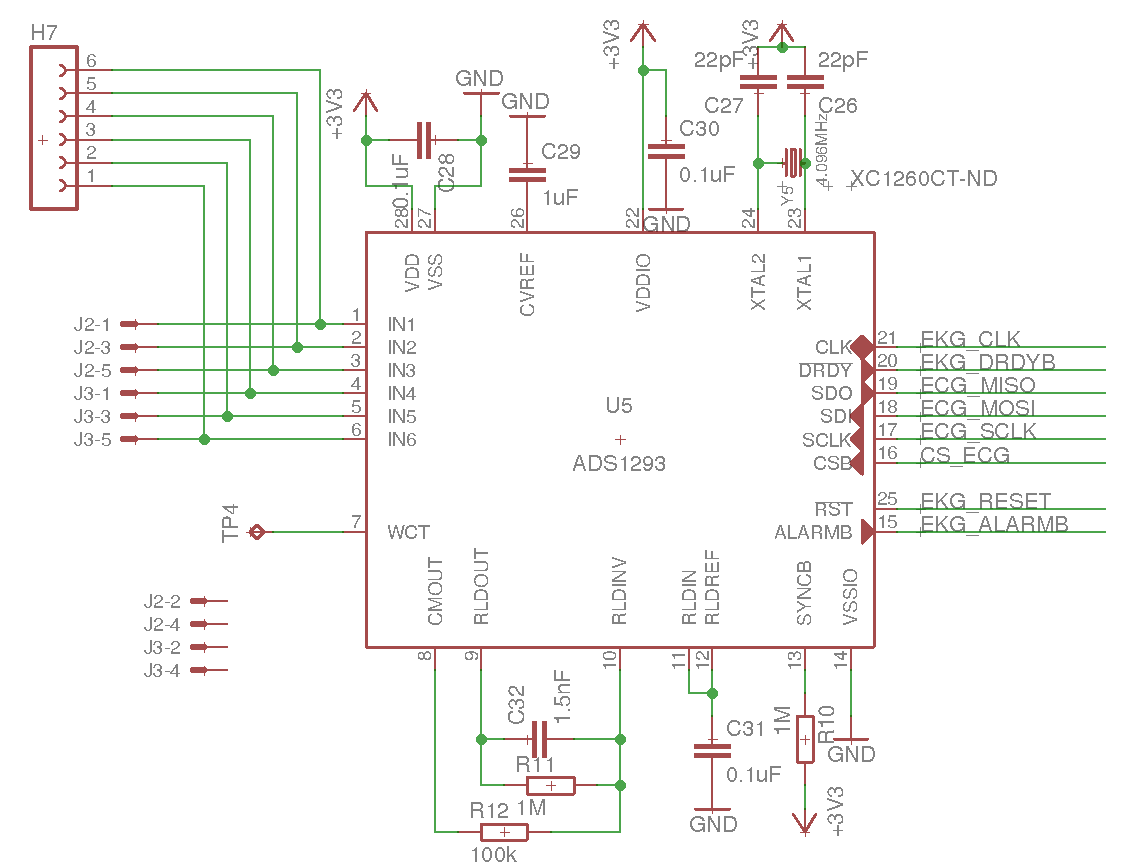
\includegraphics[scale=1,width=0.8\textwidth]{Images/Rev5_ECG.png} 
		\caption{ECG Connections for Whip Sensor}
		\label{fig:Rev5_ECG}
	\end{center}
\end{figure}

The previous WHIP prototypes made use of instrumentation amplifiers and op amps. Designs had begun to allow for adjustable gain via digitally controlled potentiometers in the feedback circuit. However, as designs were progressing a monolithic IC was released that provided all the features required in a single IC package, the ADS1293.\cite{ADS1293} This ECG front-end provides a full analog solution with software adjustable gain for up to 5 leads with Right Leg Drive (RLD). The data interface is SPI compatible and fully interrupt driven with programmable data rates. The module does require its own crystal to operate correctly. ECG lead connectors were the only other module component. ECG connectors were chosen to interface with traditional hospital leads, but were ultimately removed in favor of the snap on solution discussed in \Cref{sec:EnclosureDesign}. Hospital leads were used heavily during prototyping and validation only. Software setup of th ECG module is provided in detail in \nameref{chap:SensorConcepts}, but results in an initial configuration by the control module at power up and then provides an interrupt driven stream of data to the control module until signaled to halt.

\subsubsection{The \spo2 Module}

\begin{figure}
	\begin{center}
		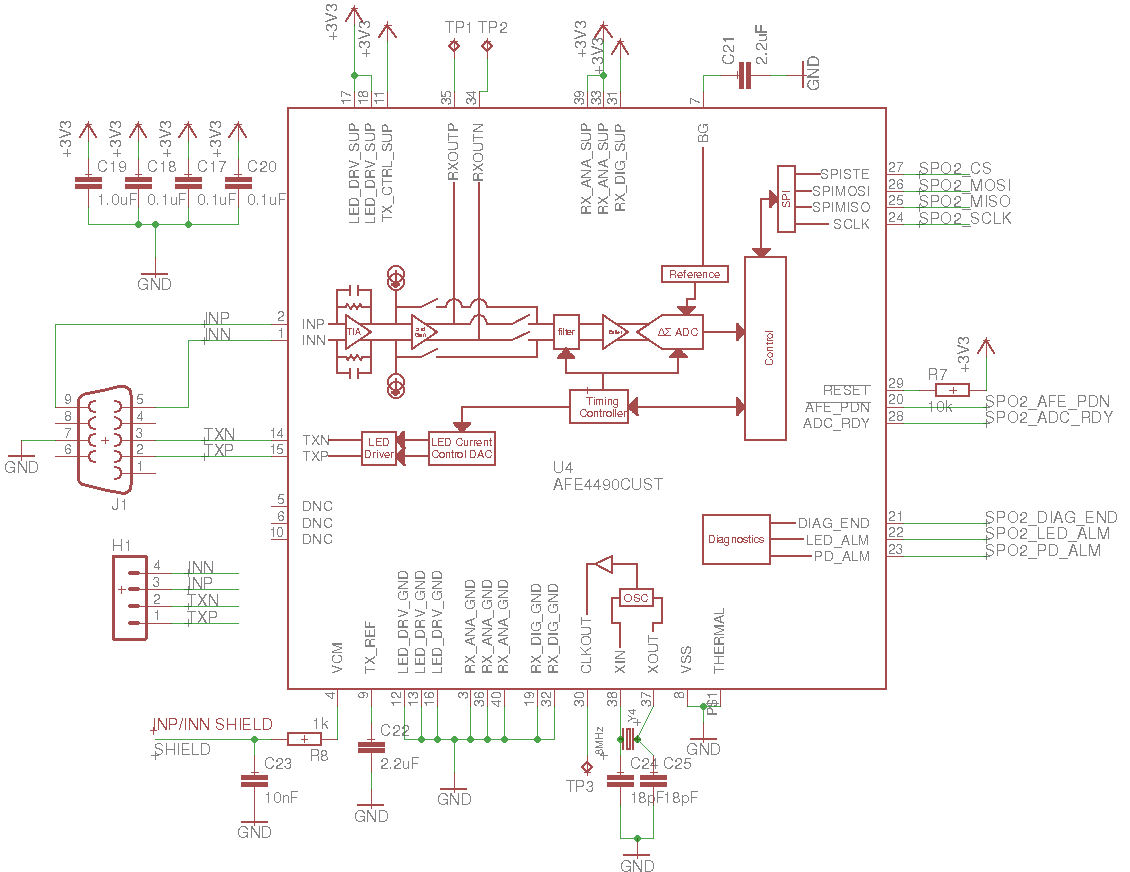
\includegraphics[scale=1,width=\textwidth]{Images/Rev5_SPO2.png} 
		\caption{\spo2 Connections for Whip Sensor}
		\label{fig:Rev5_SPO2}
	\end{center}
\end{figure}
Similar to the ECG module the discrete component implementation of the \spo2 module was replaced with a monolithic device, the AFE4490.\cite{AFE4490} The AFE4490 handles the signal multiplexing of both Red and IR LEDs, and allows software programmable gain, also over an SPI data bus. Also, like the ECG module IC the AFE4490 requires its own crystal. The last thing to mention about the \spo2 module shown in \cref{fig:Rev5_SPO2}, is the connector. The first analog PCB featured a through-hole DB9 connector was used to interface with the finger clip sensor, in subsequent designs a surface mount component was used instead. This introduced an unexpected point of failure when combined with the final PCBs and is addressed in \nameref{sec:EnclosureDesign}. The \spo2 module is provided an initial configuration by the control module at power-up and the provides and interrupt driven stream of data to the control module until told to halt.

\subsubsection{The Communication Module}
\begin{figure}
	\begin{center}
		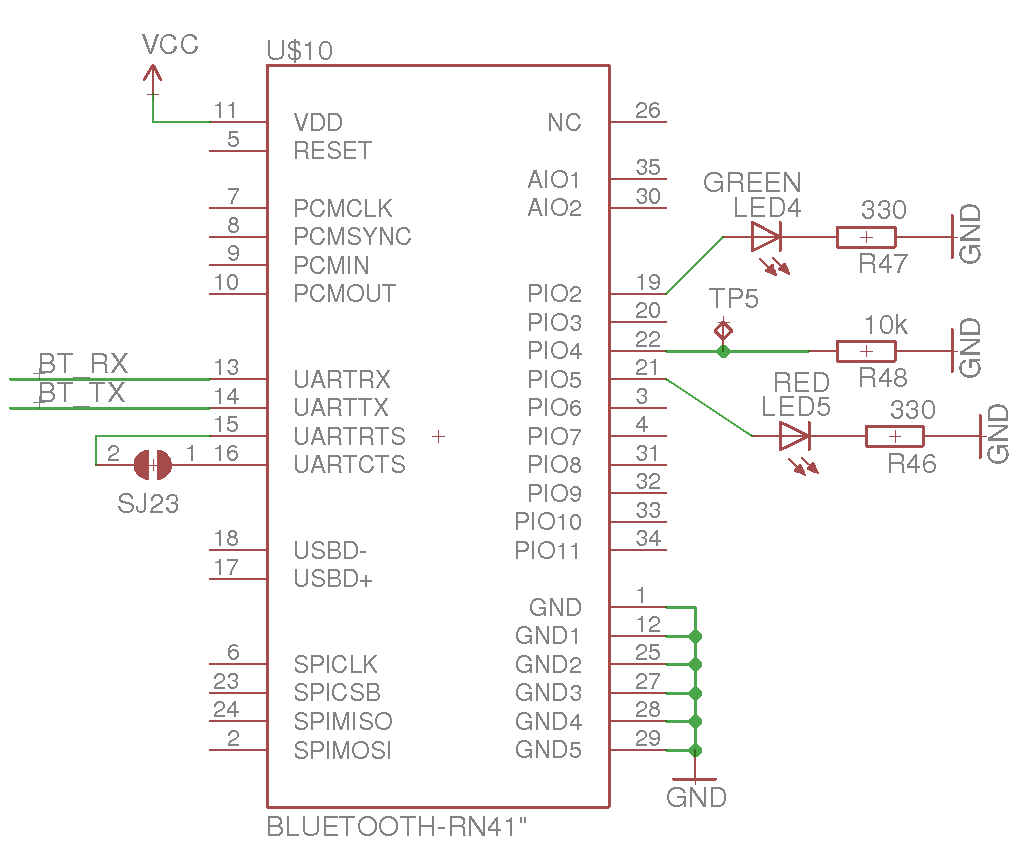
\includegraphics[scale=1,width=0.8\textwidth]{Images/Rev5_BT.png} 
		\caption{Bluetooth Serial Communication Connections for Whip Sensor}
		\label{fig:Rev5_BT}
	\end{center}
\end{figure}
The communication module implements a black box full duplex asynchronous serial connection with another device over Blue tooth. this modules design was validated in revision one and has remained unchanged since that time. 

\subsubsection{The Control Module}
% "of the Whip" - "of the Wireless Health indicator Patch"
The control module is the main brain of the WHIP. The Atmel AT32UC3B0512 provides multiple SPI channels with hardware DMA access, a full floating point calculation unit, full speed USB hardware stack, and a serial link for the communication module.\cite{AT32UC3B} The processor is new in this revision, but the UC3 family has been used for all prototypes. Additionally, since the firmware for this device was written using the Atmel Software Framework (ASF) as a hardware abstraction layer, almost all firmware code written previously was easily ported to the new processor. Due to size, the schematic for the control module has been put in \nameref{fig:FullSchematic_Sheet1}.

\subsubsection {Sub-Module Design and Testing}

\begin{figure};
	\begin{center}
		\includegraphics[scale=1,width=0.45\textwidth]{Images/ECGBreakout.png} 
		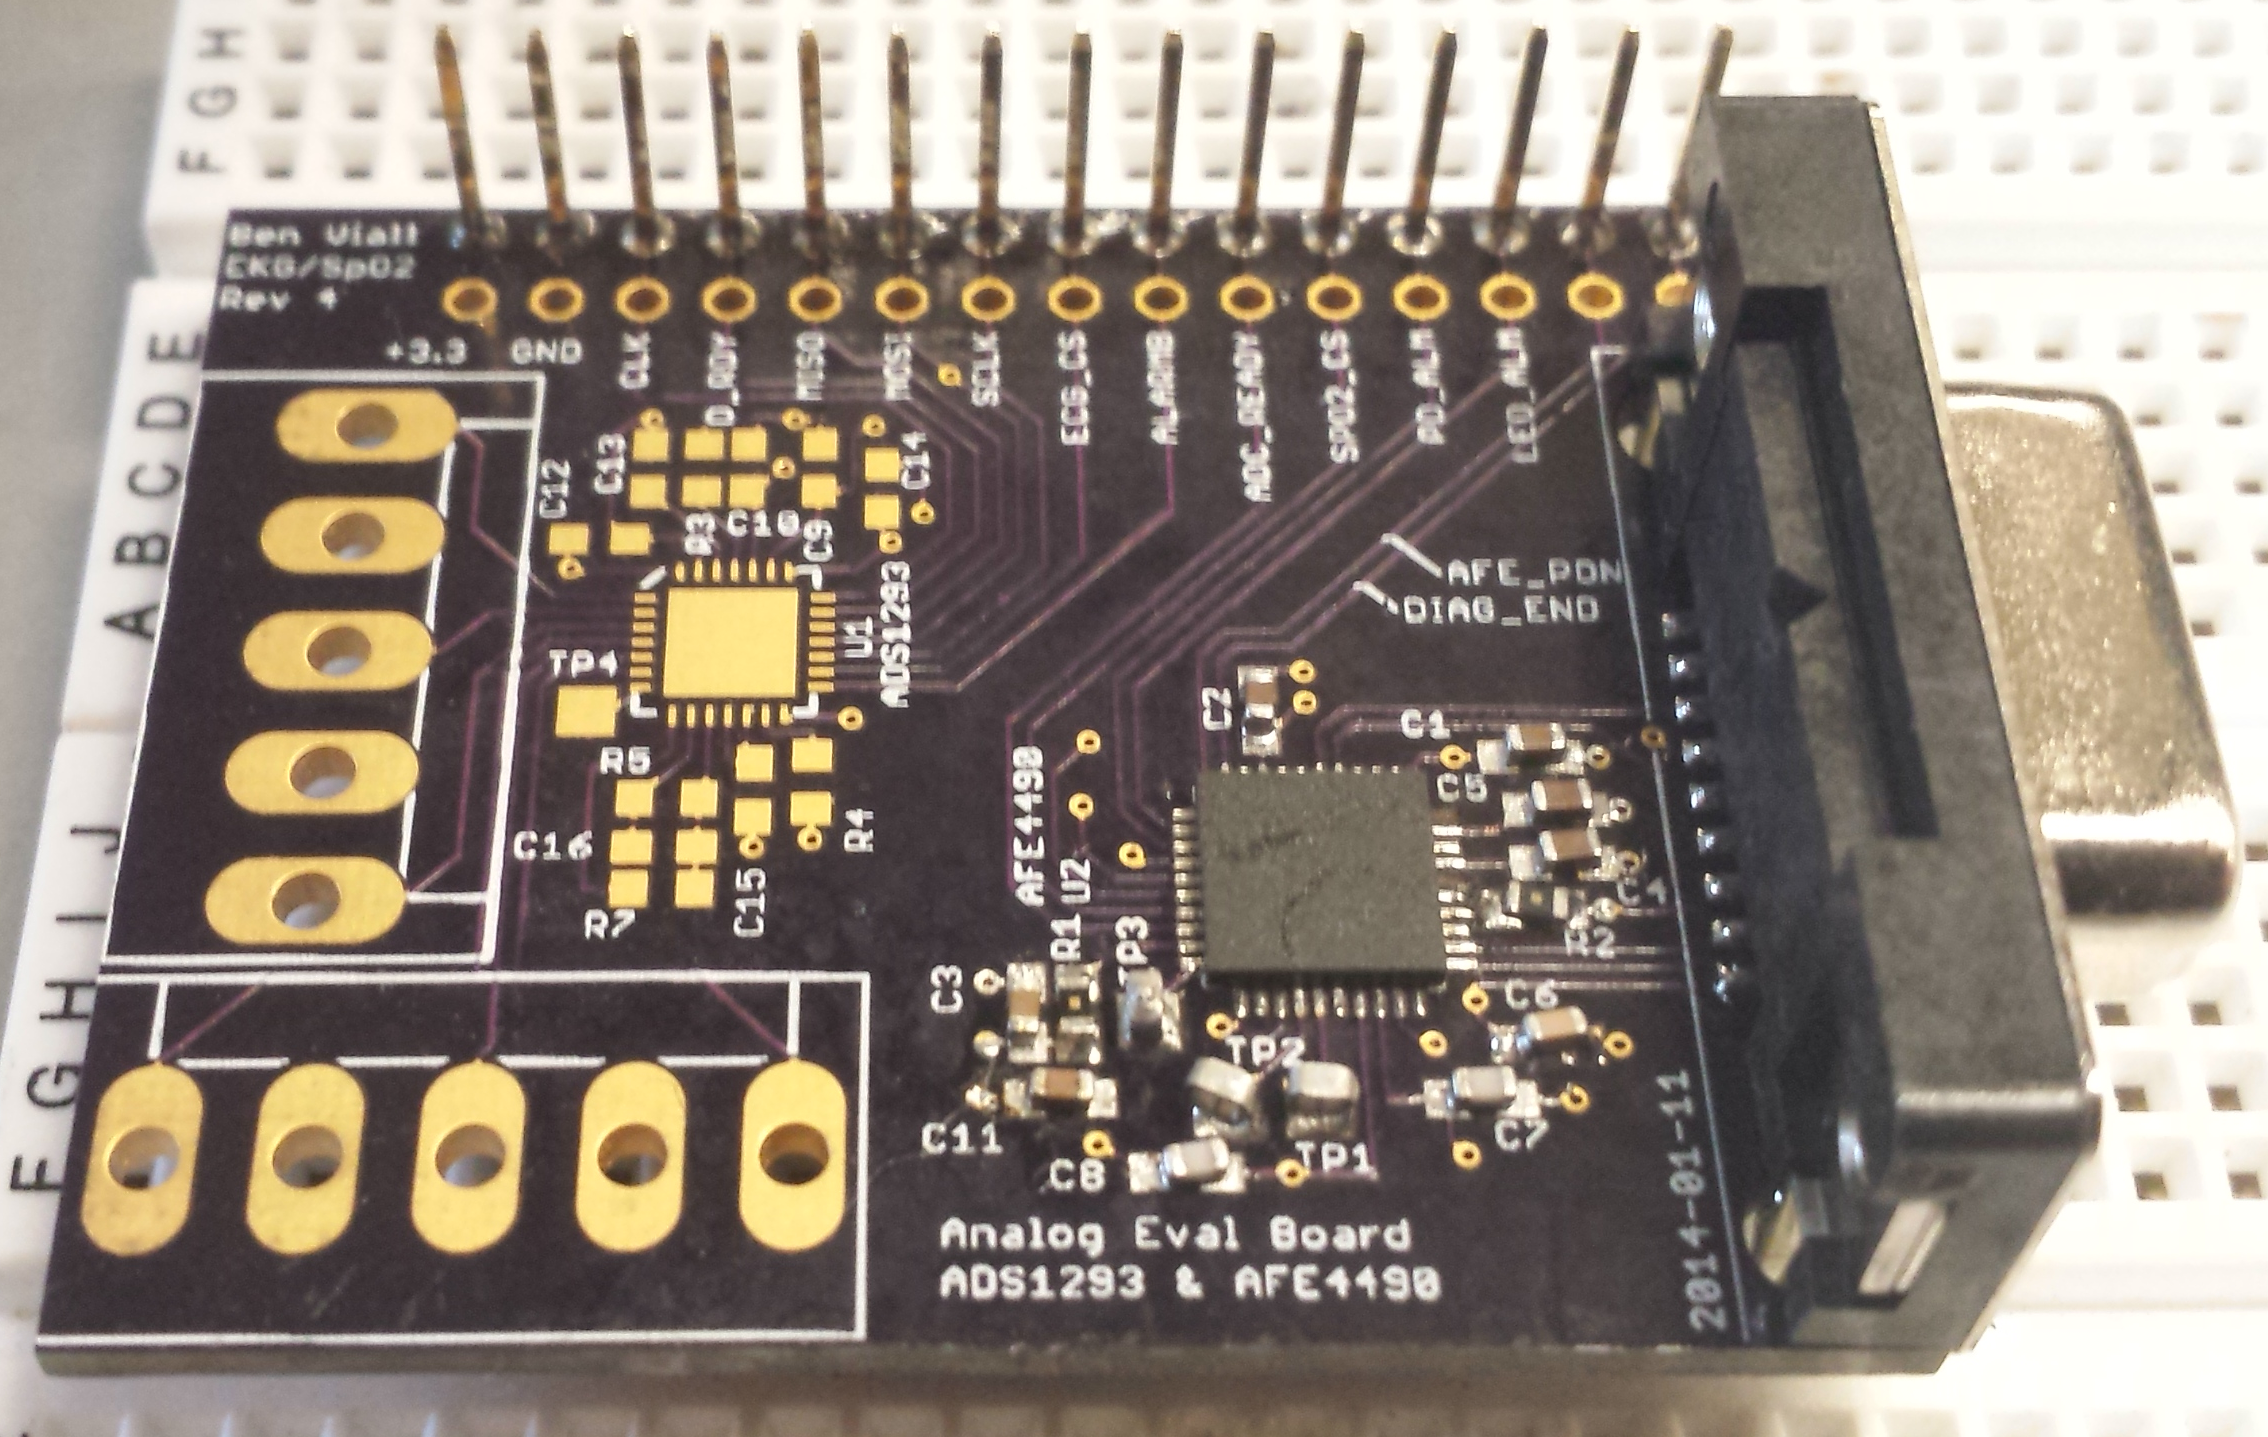
\includegraphics[scale=1,width=0.45\textwidth]{Images/SPO2Breakout.png} 		
		\caption{Populated Breakout Boards for ECG and \spo2 Devices}
		\label{fig:Breakouts}
	\end{center}
\end{figure}

Time is always a factor in any production, to start the trial as soon as possible integration was done in only two steps, first the ECG and \spo2 Modules were fabricated to a PCB and confirmed to meet requirements. This type of PCB is often referred to as a breakout board. The signals are brought from a tight pin pitch device to 0.100 inch headers for breadboarding. An ATMega32U4 \cite{ATMEGA32U4} was tasked with supplying configuration data to the analog front end chips, then consuming the data as it was delivered for basic testing of the design. A basic heart monitor was created as proof of concept to showcase the validity of the design by adding an OLED module to display a real-time EKG shown in \cref{fig:Breakout Test}. This design was brought to the UMASSD fitness center, where it survived a burn in test on a subject running on a treadmill for approximately 30 minutes. 
The treadmill test utilized version two of the breakout board since the first breakout PCB demonstrated a serious problem with the artwork for the \spo2 module; the AFE4490 chip didn't fit in the space provided. Another revision was sent for production while work continued with the ECG. The advantage of creating a breakout board for the two modules was in the freedom to confirm every connection. Several of the control and status signals were unclearly documented. Once the breakout board arrived, the signals could be experimented with, using hookup wire. Despite the problems with PCB artwork on the breakout board, ultimately fabricating breakout boards saved both time and money, because the footprint error was discovered earlier in the design process.

\begin{figure};
	\begin{center}
		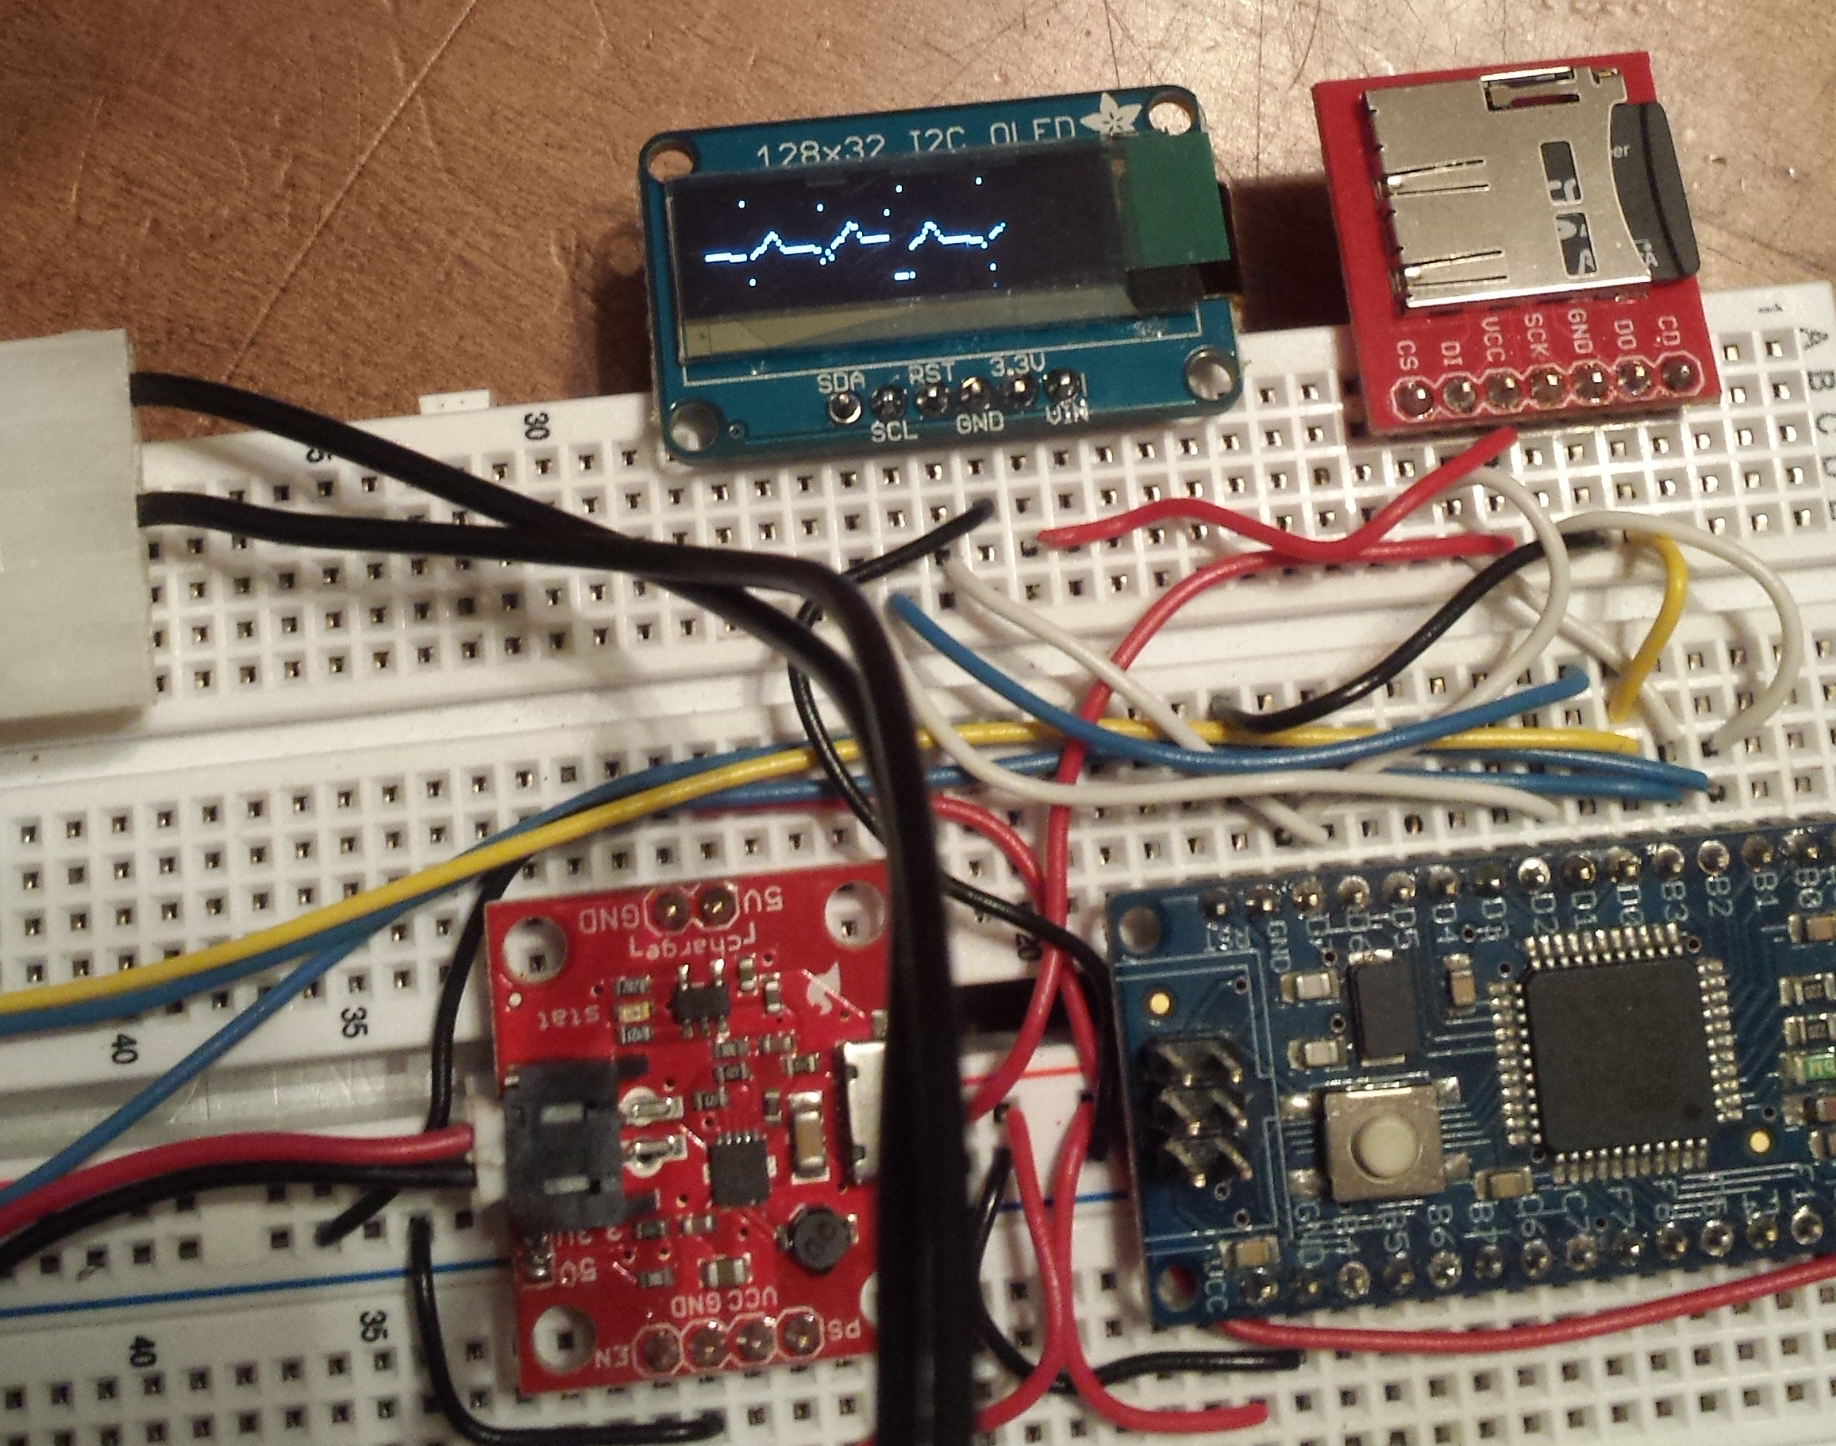
\includegraphics[scale=1,width=0.45\textwidth]{Images/BreadBoardTest.png} 		
		\caption{Test Rig for ECG and \spo2 Breakout Board Showing Real-time ECG Trace}
		\label{fig:Breakout Test}
	\end{center}
\end{figure}


\subsection{Printed Circuit Board (PCB) Layout}
After all modules had been designed in schematic capture, the design for the PCB began. The physical location of connectors was the driving force in the layout process. Given the board manufacturer in use at the time of production, the physical size of the board was set to 100 mm by 50 mm. The ECG and \spo2 transducer connections as well as the USB and SD card port were required to be on the board perimeter. Each module had its components grouped near each other and were routed to the module level. The modules were then positioned near their final destinations and inter-module routing occurred. the final Layout is shown in \Cref{fig:FullLayout}.

\begin{figure}[ht]
\begin{center}
	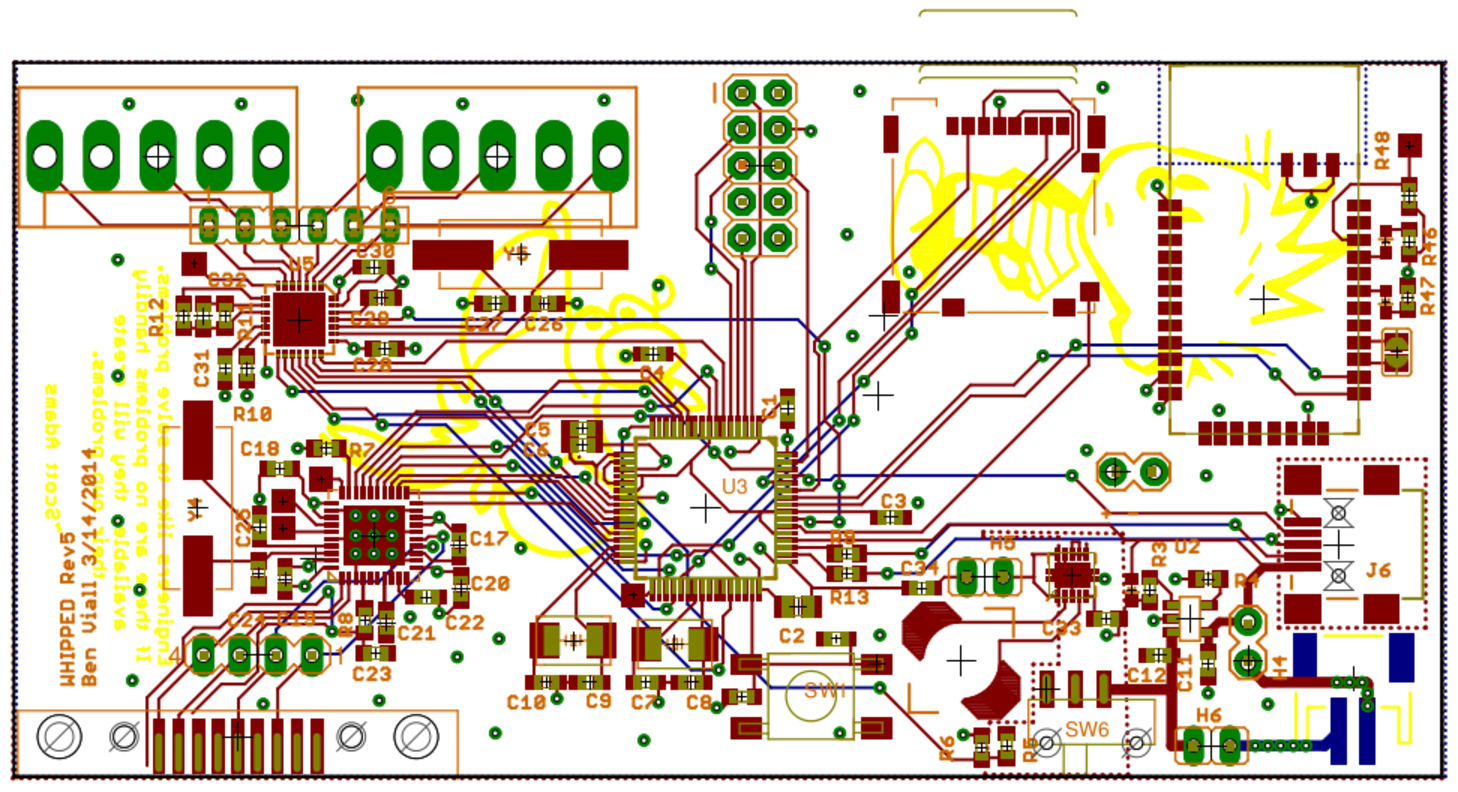
\includegraphics[angle=0,scale=1,width=1\textwidth]{Images/rev1D_PCB_cropped.pdf} 
	\caption{Full PCB Layout Top and Bottom}
	\label{fig:FullLayout}
\end{center}
\end{figure}

Some modules in the WHIP design required special consideration beyond what could be recorded during schematic capture. The bluetooth module required the antenna to have no traces or copper pour beneath it's antenna area. this pullback can be seen on the upper right corner of all gerber layers in  \Cref{chap:PCB_LAYOUT}: \nameref{chap:PCB_LAYOUT}. Also, the SD module's physical placement was very sensitive; and needed to be placed close enough to the edge of the board to allow for card ejection but far enough away to prevent accidental ejection. Finally, the \spo2 module application note recommended guard traces to prevent noise that were routed around the sensitive signal traces. 


\subsection {Final Prototype Construction}
The second stage of integration occurred on the final WHIP PCB. Unlike production PCB assembly, the first prototype was not assembled all at once. First the power module was soldered together, and tested with a multimeter. This supply must have a load to provide proper regulation, therefore a 10,000-Ohm resistor was bridged across VCC and GND. The power system was validated as working only after adding this load resistor and confirming 3.3 Volts. The charging system was then validated by plugging a partially drained LIPO battery into the board with a USB cable connected to a computer. If the indicator 'LED1' lights, the charging circuit is validated. 

Now that the entire power module is soldered all other tests are prefaced by an additional test. Before reapplying power after any soldering, a multimeter should be used to check for accidental shorts between VCC and GND. Additionally, it is often useful to perform the ``finger test'' when powering new peripherals. The finger test involves placing a finger on the top of an IC package as you power the PCB. If there is an error in soldering, or wiring, the chip will, more than likely, heat up, your finger can detect this thermal event and power can be disconnected, hopefully before any damage is done, either to your power supply,your finger, or your new component. These tests will not be mentioned in the descriptions below, but are still performed before power is applied during every test.

The communication module was next to be validated, after removing all power, the communication module is added to the PCB. When power was applied, an attempt was made to connect to the module using an android phone. If pairing is successful, an additional test is performed. Opening a serial communication terminal on the phone ``+++'' is sent across the link if the module responds with ``OK'' then the Bluetooth module has entered over the air (OTA) configuration mode. Power can now be removed and the control module and Memory Module can be soldered on. 

The remaining tests all involve running parts of a validation firmware. The firmware runs on the microprocessor and exercises each of the other modules and provides an automated readout on the serial port. The JTAG module inside the microprocessor must be running o run the remaining test. This is tested by attaching the JTAG programmer to the board and attempting to read the device ID. if the test fails there is likely a soldering error, such as two or more pins shorted together, or a pin the is not soldered directly to the pad. A multimeter in continuity mode can find these errors quickly. 

\begin{figure}[ht]
\begin{center}
	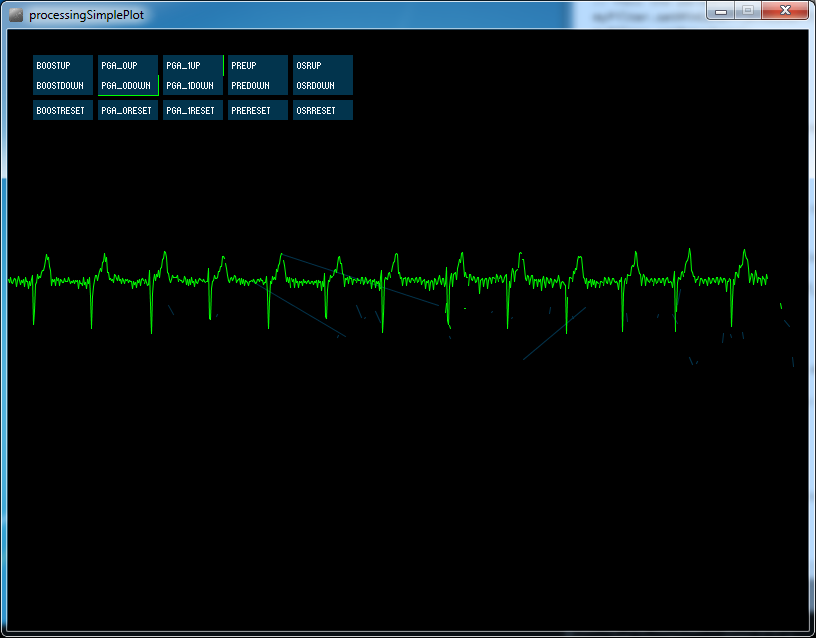
\includegraphics[angle=0,scale=1,width=1\textwidth]{Images/ECG_processingSketch.png} 
	\caption{Successful Test of `ECGcheck' Firmware}
	\label{fig:ECG_Test_Pass}
\end{center}
\end{figure}

Once firmware can be loaded into the microprocessor, insert an SD card into the device, power does not need to be removed. Run the SDcardcheck firmware and observe the serial output. The test will have PASS/FAIL result. Upon getting a PASS, disconnect the power and solder the \spo2 Module, and load the SPO2check firmware and the PC side software. Connect the finger clip to the board and affix it to your finger. Connect the PC software to the device via the local COM port and hit run. You should see a two graphs representing your Red and IR Photoplethysmograph. Finally, disconnect the power.

Finally, solder the ECG module to the PCB. Load the ECGcheck firmware and accompanying PC side software. Connect the 3 ECG leads to a patient or other signal source. Connect the PC software to the device via the local COM port and hit run. You should see a rolling graph of your ECG similar to \cref{fig:ECG_Test_Pass}. Now, all components should be on the board, and have been validated.


Once the first prototype was validated, six boards at a time were populated at once. First solder paste was applied to all boards using a stencil. Then, all components were manually populating. Finally, the boards were soldered in a custom made reflow oven. The results are shown in \cref{fig:ReflowedBoards}. Each board was then checked for shorts and reworked as needed.

\begin{figure}[ht]
\begin{center}
	\includegraphics[angle=0,scale=1,width=1\textwidth]{Images/BoardsSoldered.png} 
	\caption{Fully Populated Boards, Just Out of the Reflow Oven}
	\label{fig:ReflowedBoards}
\end{center}
\end{figure}


\section {Enclosure Design}
\label{sec:EnclosureDesign}
Part of the research component of this dissertation was to evaluate methods, and make design choices, to promote the usability of the  proposed technology; specifically to encourage adoption by people over the age of 65. The next step in the integration process was to create an apparatus, that could be easily put on by a patient and provide reliable positioning of the electrodes every time. An important requirement of the physical design was to provide long term wearibility, the device should be worn anytime the user is awake. One exception is any time the device may be exposed to water. Deciding the device not be waterproof for the current trial simplified the design. The first goal of the enclosure, then, was to make it as comfortable as possible while maintaining overall functionality. The apparatus was designed in two parts: the chest strap, and the electronics enclosure. 




\subsection {Chest Strap}
\begin{figure}[ht]
\begin{center}
	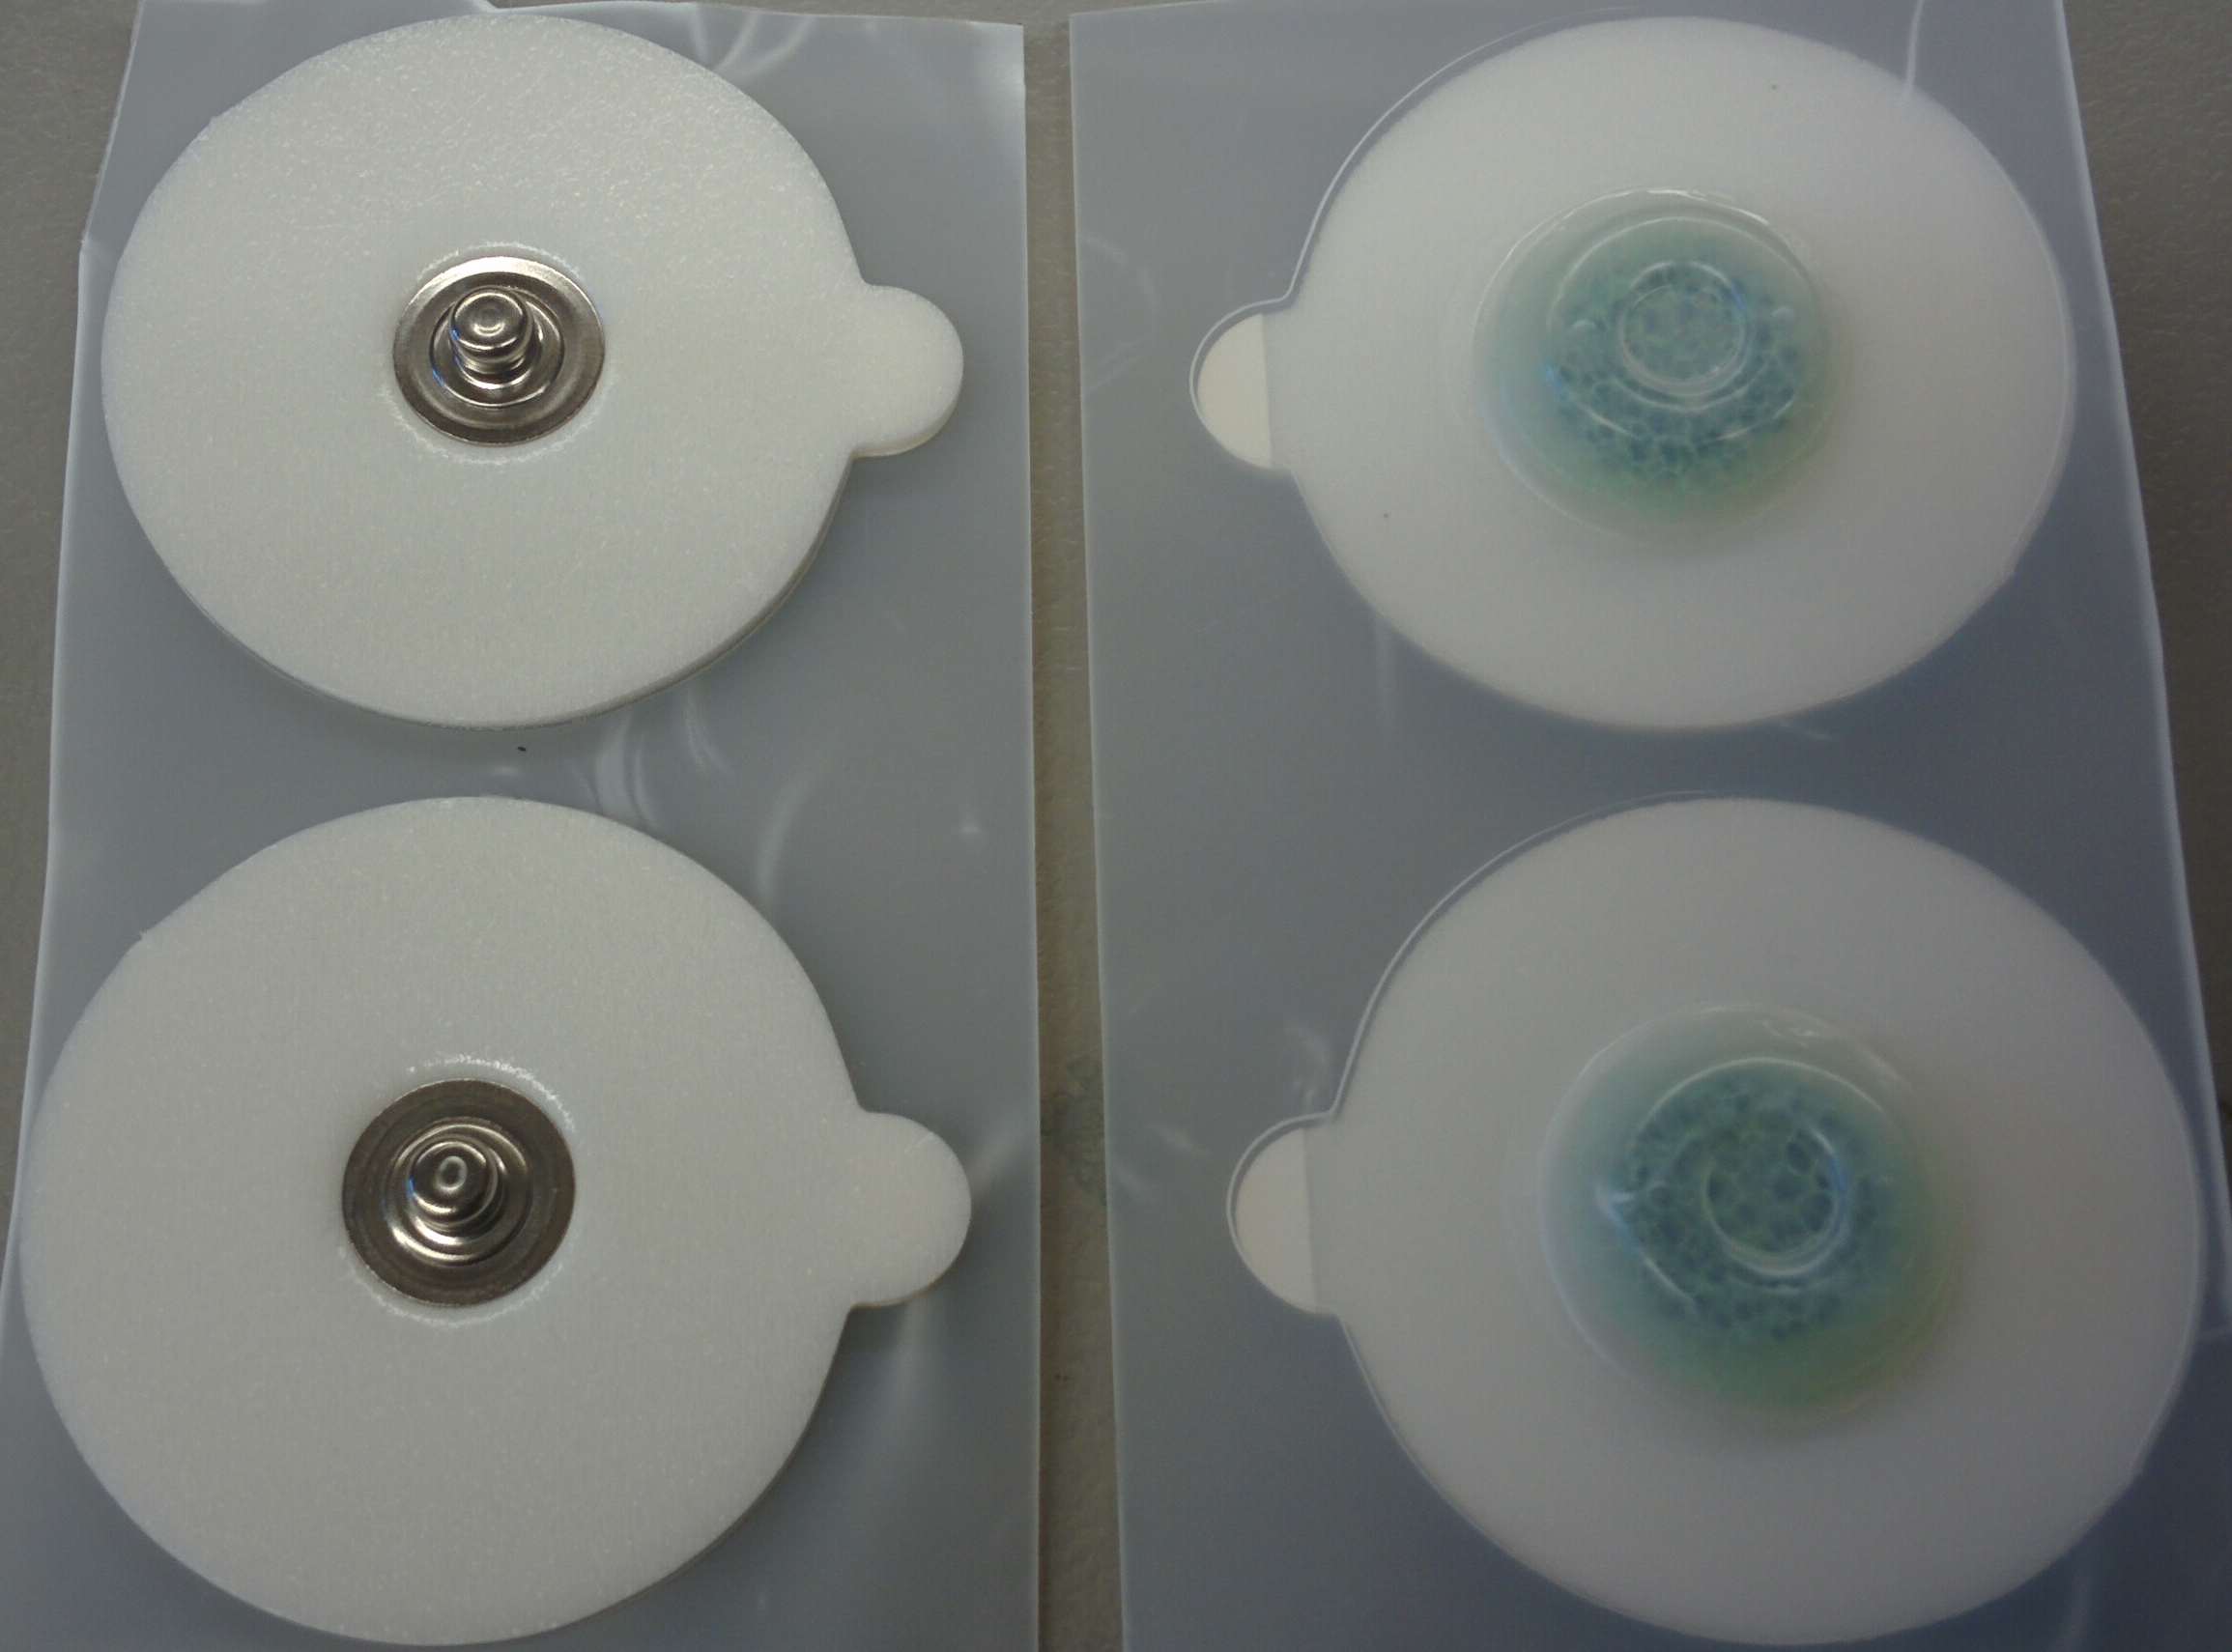
\includegraphics[angle=0,scale=1,width=.5\textwidth]{Images/Electrodes.png} 
	\caption{Sticky Electrodes, Top and Bottom}
	\label{fig:Electrodes}
\end{center}
\end{figure}
Initial testing of the device was performed in a laboratory setting using a sensor board equipped with rubber feet to prevent shorting any exposed traces on the underside of the PCB. A temporary cable was constructed the connected to traditional pre-moistened sticky electrodes shown in \cref{fig:Electrodes}. This design was scrapped after areas of irritation began to appear on the engineers after several days of ripping off and reapplying electrodes. It was clear that wet electrodes would not be appropriate for long term use.

The next design replaced sticky electrodes with dry contacts held in place by means of a stretchable fabric strap. Each strap was fitted with a buckle to make it easy to both put on and take off. Three electrodes, made of velostat, a conductive flexible material often found in commercial fitness bands, were sewn into the strap and connected with fabric snaps to the sensor board. This design functioned well electrically, however no fabric could be sourced that offered the correct combination of traits to make it both feel comfortable, and support the sensor board. This metric, of feeling comfortable, was qualitative only. No quantitative data on feel was collected during the design process.

After several iterations, that never produced a qualitative approval by testers, off the shelf straps designed for runners, specifically the polar heart rate monitor strap was used. The heart rate sensor hardware made by polar was not used, only the strap. The polar strap provided a comfortable feeling strap that could also support the weight of the sensor board and battery. However, these straps only provided two electrodes. A third electrode was added using the velostat material from the second prototype. The final strap connection is shown in \cref{fig:polar_3rdSnap}.

\begin{figure}[ht]
\begin{center}
	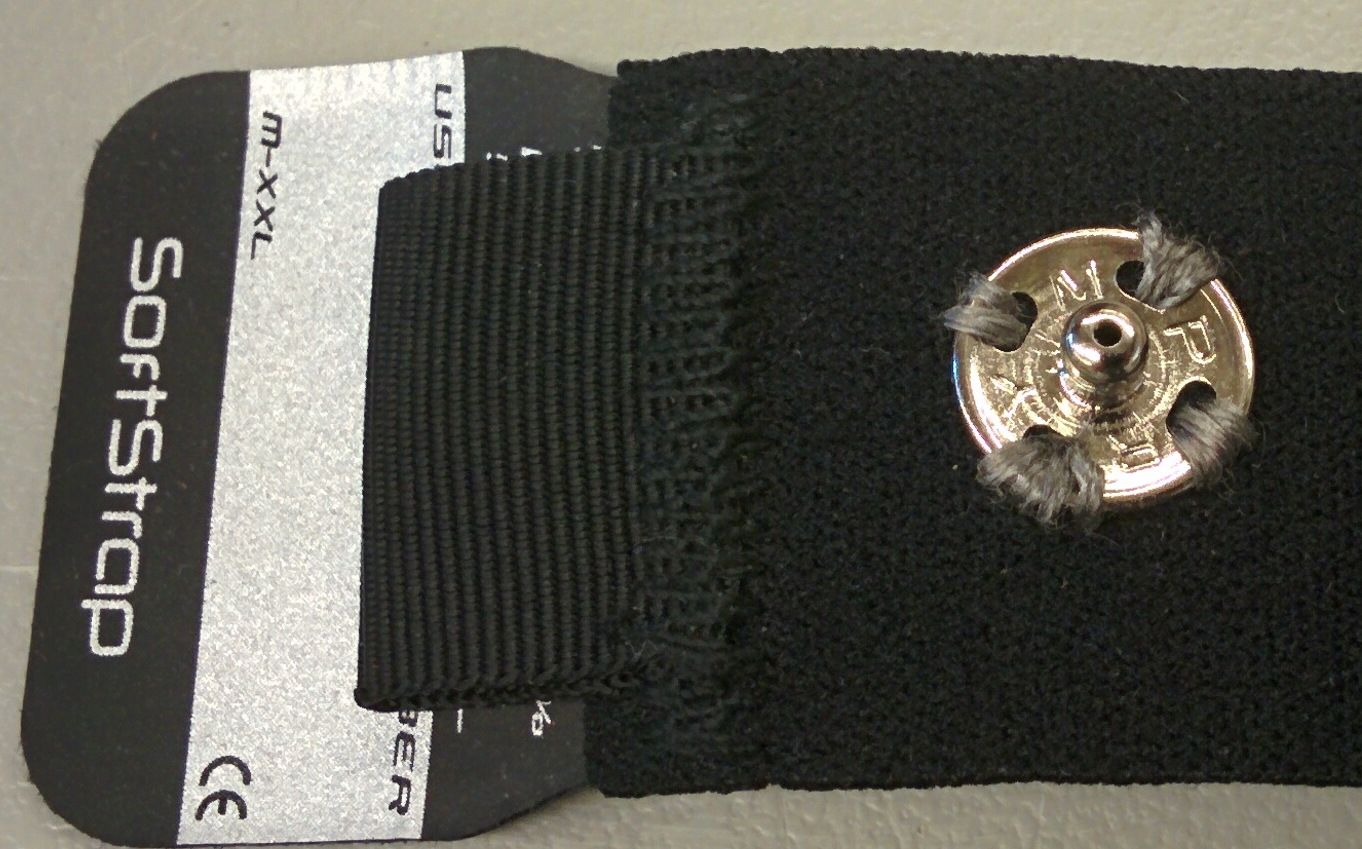
\includegraphics[angle=0,scale=1,width=.51\textwidth]{Images/Polar_top.png} 
	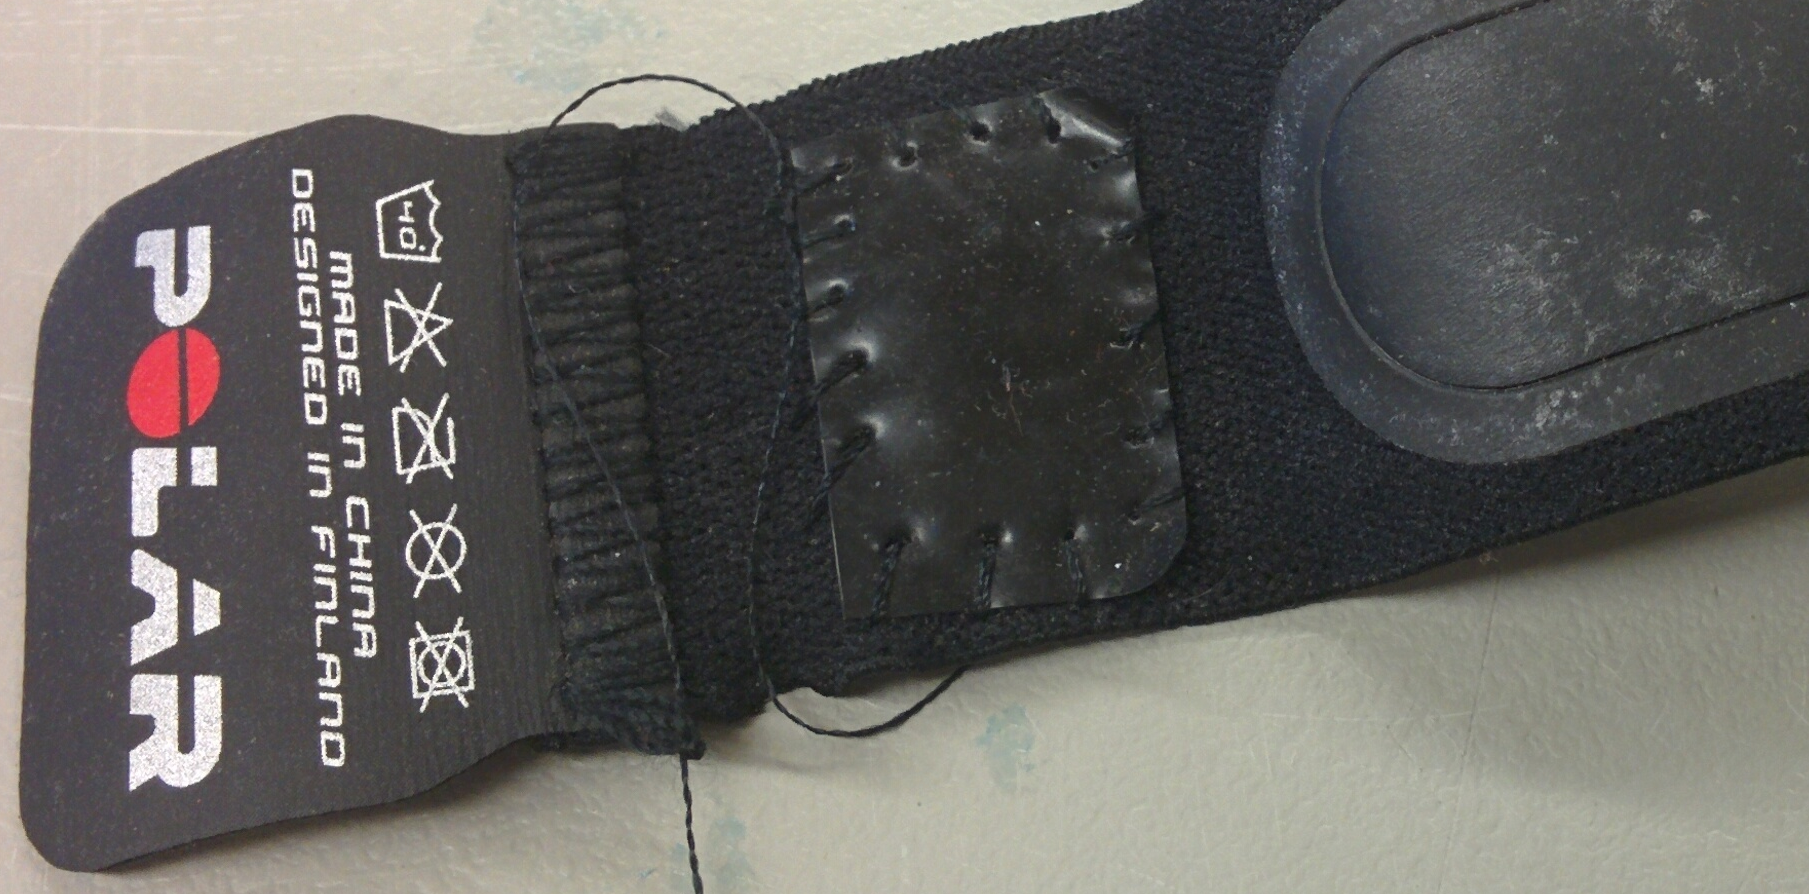
\includegraphics[angle=0,scale=1,width=.51\textwidth]{Images/Polar_bottom.png}
	\caption{Third Electrode, Sewn using Conductive Thread and Fabric}
	\label{fig:polar_3rdSnap}
\end{center}
\end{figure}

 

\begin{figure}[ht]
 \begin{center}
  \includegraphics[scale=1,width=0.8\textwidth]{Images/Rev5Assembled.png} 
  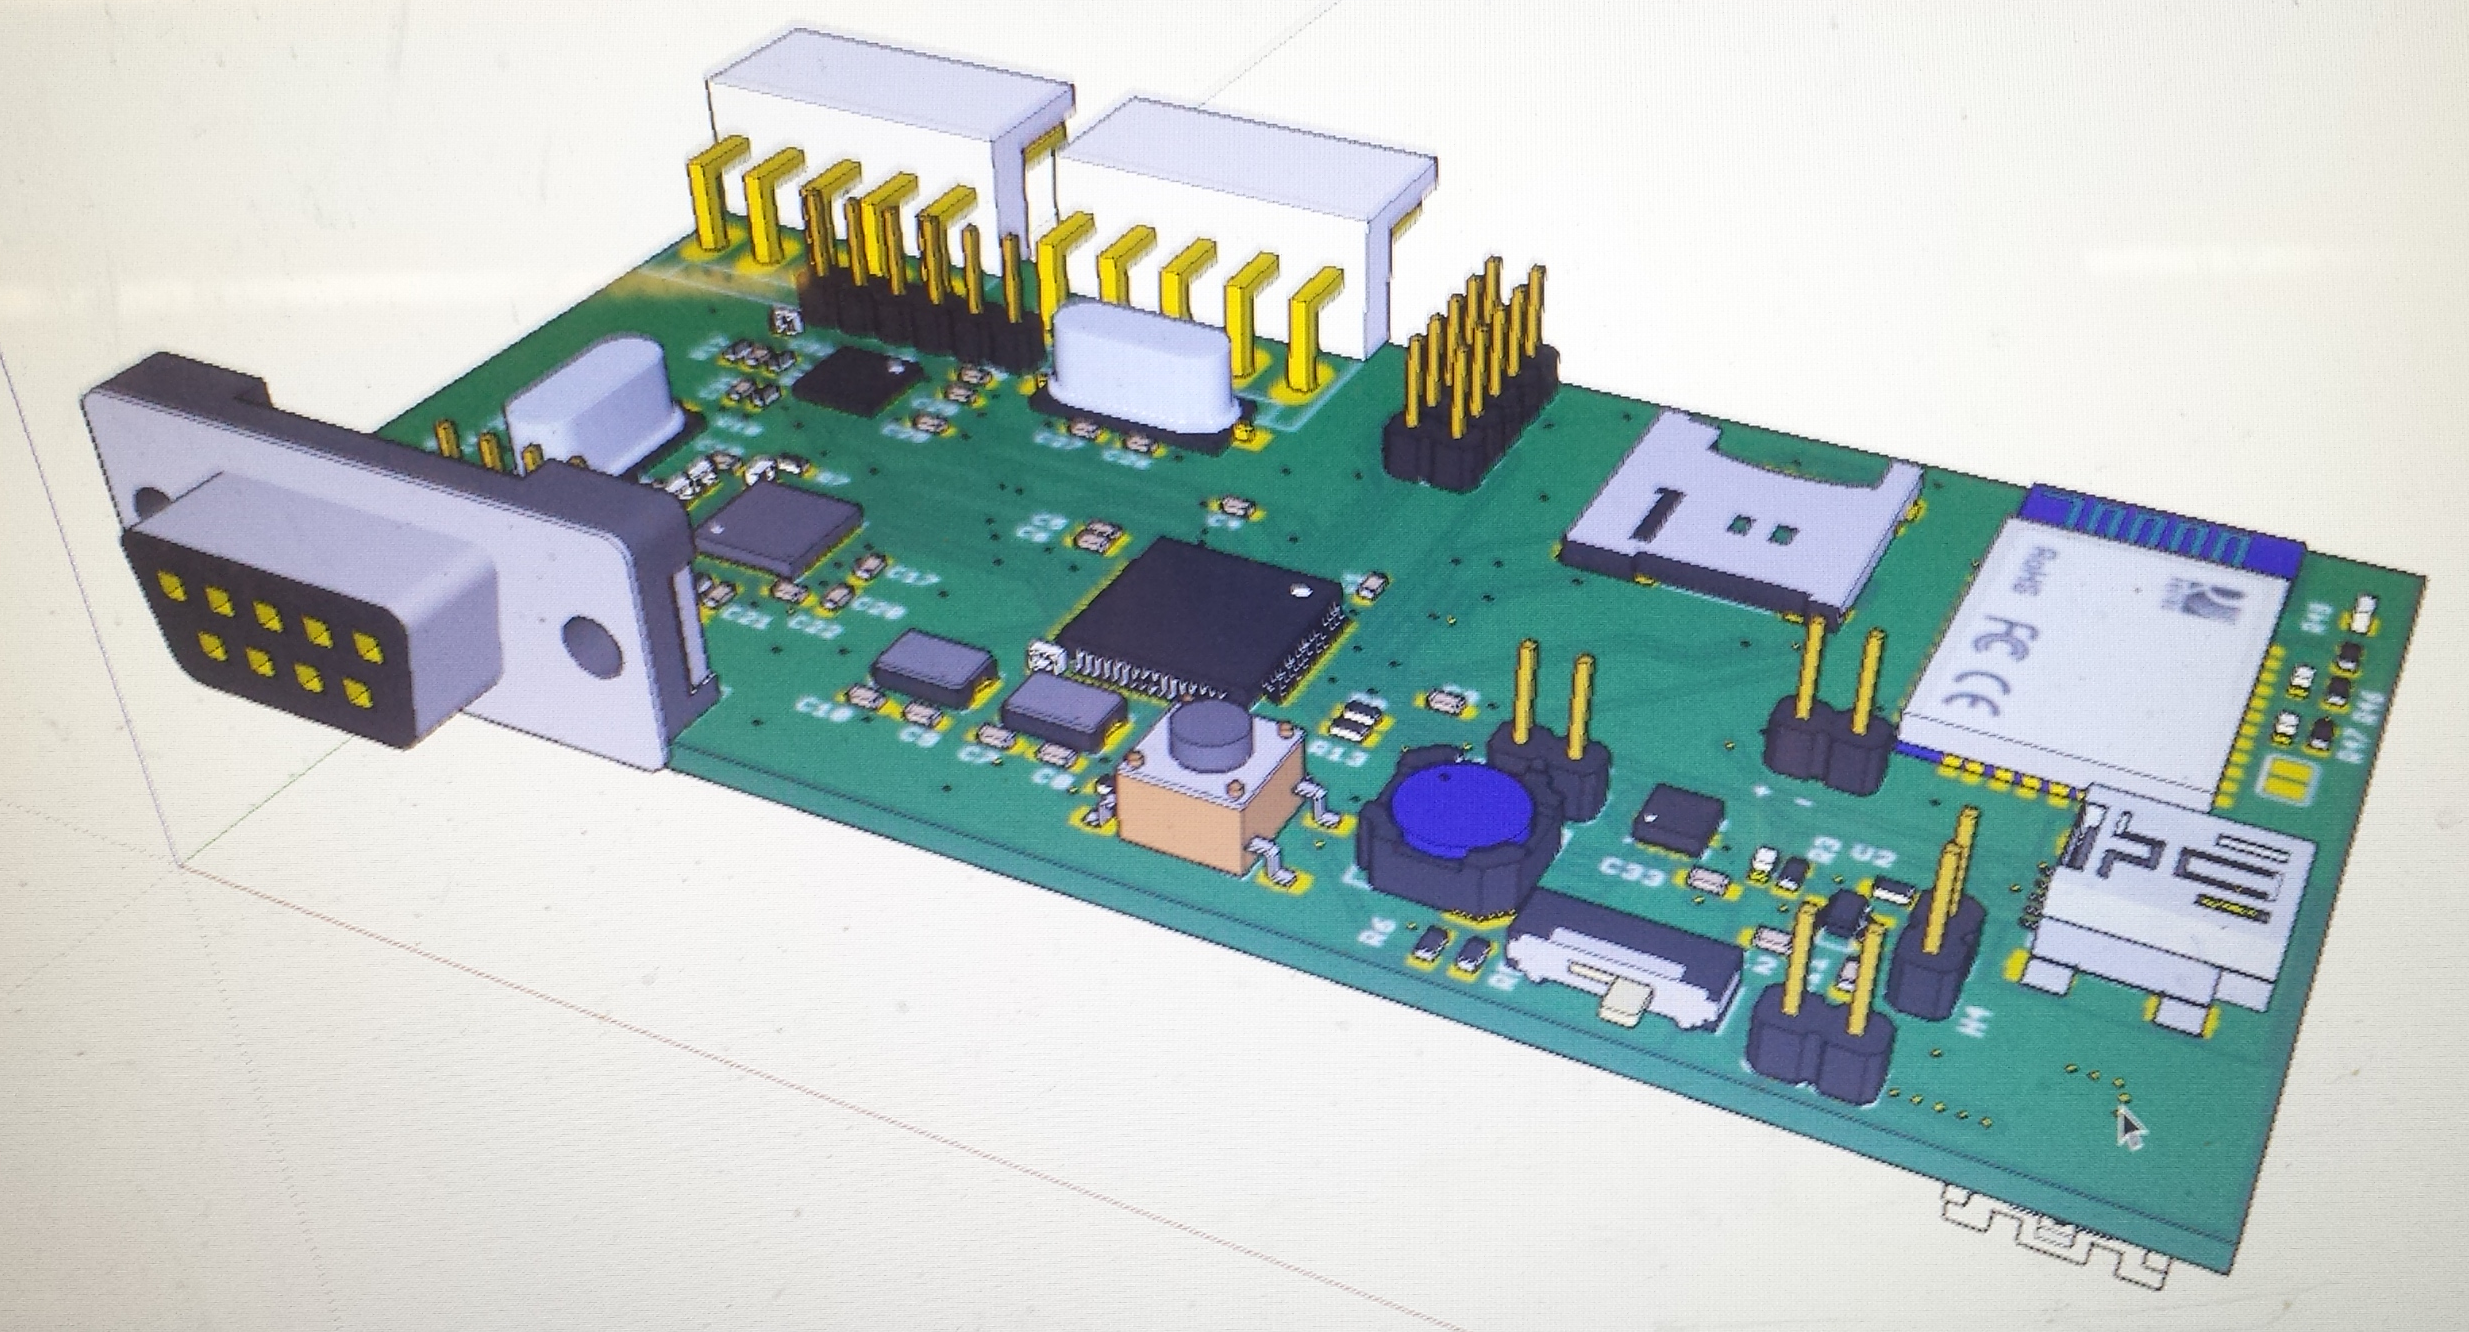
\includegraphics[scale=1,width=0.8\textwidth]{Images/Rev5_prerender.png} 
  \caption{Populated PCB vs 3D Render}
  \label{fig:PCBvsRender}
 \end{center}
\end{figure}

\subsection {3D Printed Enclosure}
The electronics enclosure served several purposes, first protecting all sensitive components from external damage. Second, providing clear access to ports of interest, including: charging port, sd card, ECG, and \spo2 ports. Lastly, keeping all components of the design enclosed together physically. 

All enclosure designs were 3d printed. 3d printing takes a digital 3d model and creates a physical object, either out of an extruded material such as plastic or wood, a process known as Fused Deposition Modeling (FDM), or by repeatedly adding a thin layer of small particles,or resin, and using a laser to selectively melt those particles to the component underneath (SLS). Both methods are common in prototyping and each has its own advantages that are not the focus of this dissertation. A Lulzbot Taz4 \cite{LULZBOT} was used to create the models used in this dissertation. The Taz4 is a FDM type machine, all models were created out of Acrylonitrile butadiene styrene (ABS) plastic. ABS was chosen for its high strength properties. 3d printing the enclosures allowed us to rapidly change the design, sometimes several times a day, and get immediate physical feedback on the design. There is no clear number of how many prototype stages were used in the design as a result. However, the following paragraphs will explain the design decisions made,from first prototype, to final prototype enclosure.


First we should discuss how the enclosure was designed. All models were created using SketchUp\cite{Sketchup}. The choice of modeling software stemmed from the existing PCB work-flow. EagleCad, the PCB design software used to make the sensor PCB, allows custom scripts or User Language Programs (ULPs) to automate tasks or augment features of the program, one available ULP allows an export of the board directly into SketchUp. The basic export only provides a 3d model of the PCB without any components on it. however, if a 3d model of each component type is available, a fully populated PCB is imported into SketchUp. A fully populated PCB model was used, not just for enclosure design, but also for checking the clearances between components before the board was fabricated. Substantial effort was put into creating 3d models of components based on the mechanical drawings from the component data-sheets. As shown in \Cref{fig:PCBvsRender} the fully populated board is well represented by the 3d model. Using a generated 3d model allowed the designer to provide tight tolerances for the overall enclosure design. 

The first enclosure was a simple box designed to hold the unpopulated PCB. Notable features of this first board included retaining clips above the board, rounded corners, integrated standoffs, and a compartment for the battery below the PCB. This was the first 3d printed object made for this project, and was used as a basic shakedown of the 3d printing process shown in. The utility of 3d printing was made immediately clear once the first prototype was printed. The PCB fit snuggly and did not move once seated. Indeed, once it was in it was difficult to get out. The second design change needed was to accommodate the battery. The standoffs were spaced too closely together to fit the battery. Testing this prototype required two standoffs be cut from the plastic model and can be seen on the left side of the enclosure in  \Cref{fig:enclosure1}. This ``modify-after-print'' approach was invaluable at each stage of the design.

\begin{figure}[ht]
 \begin{center}
  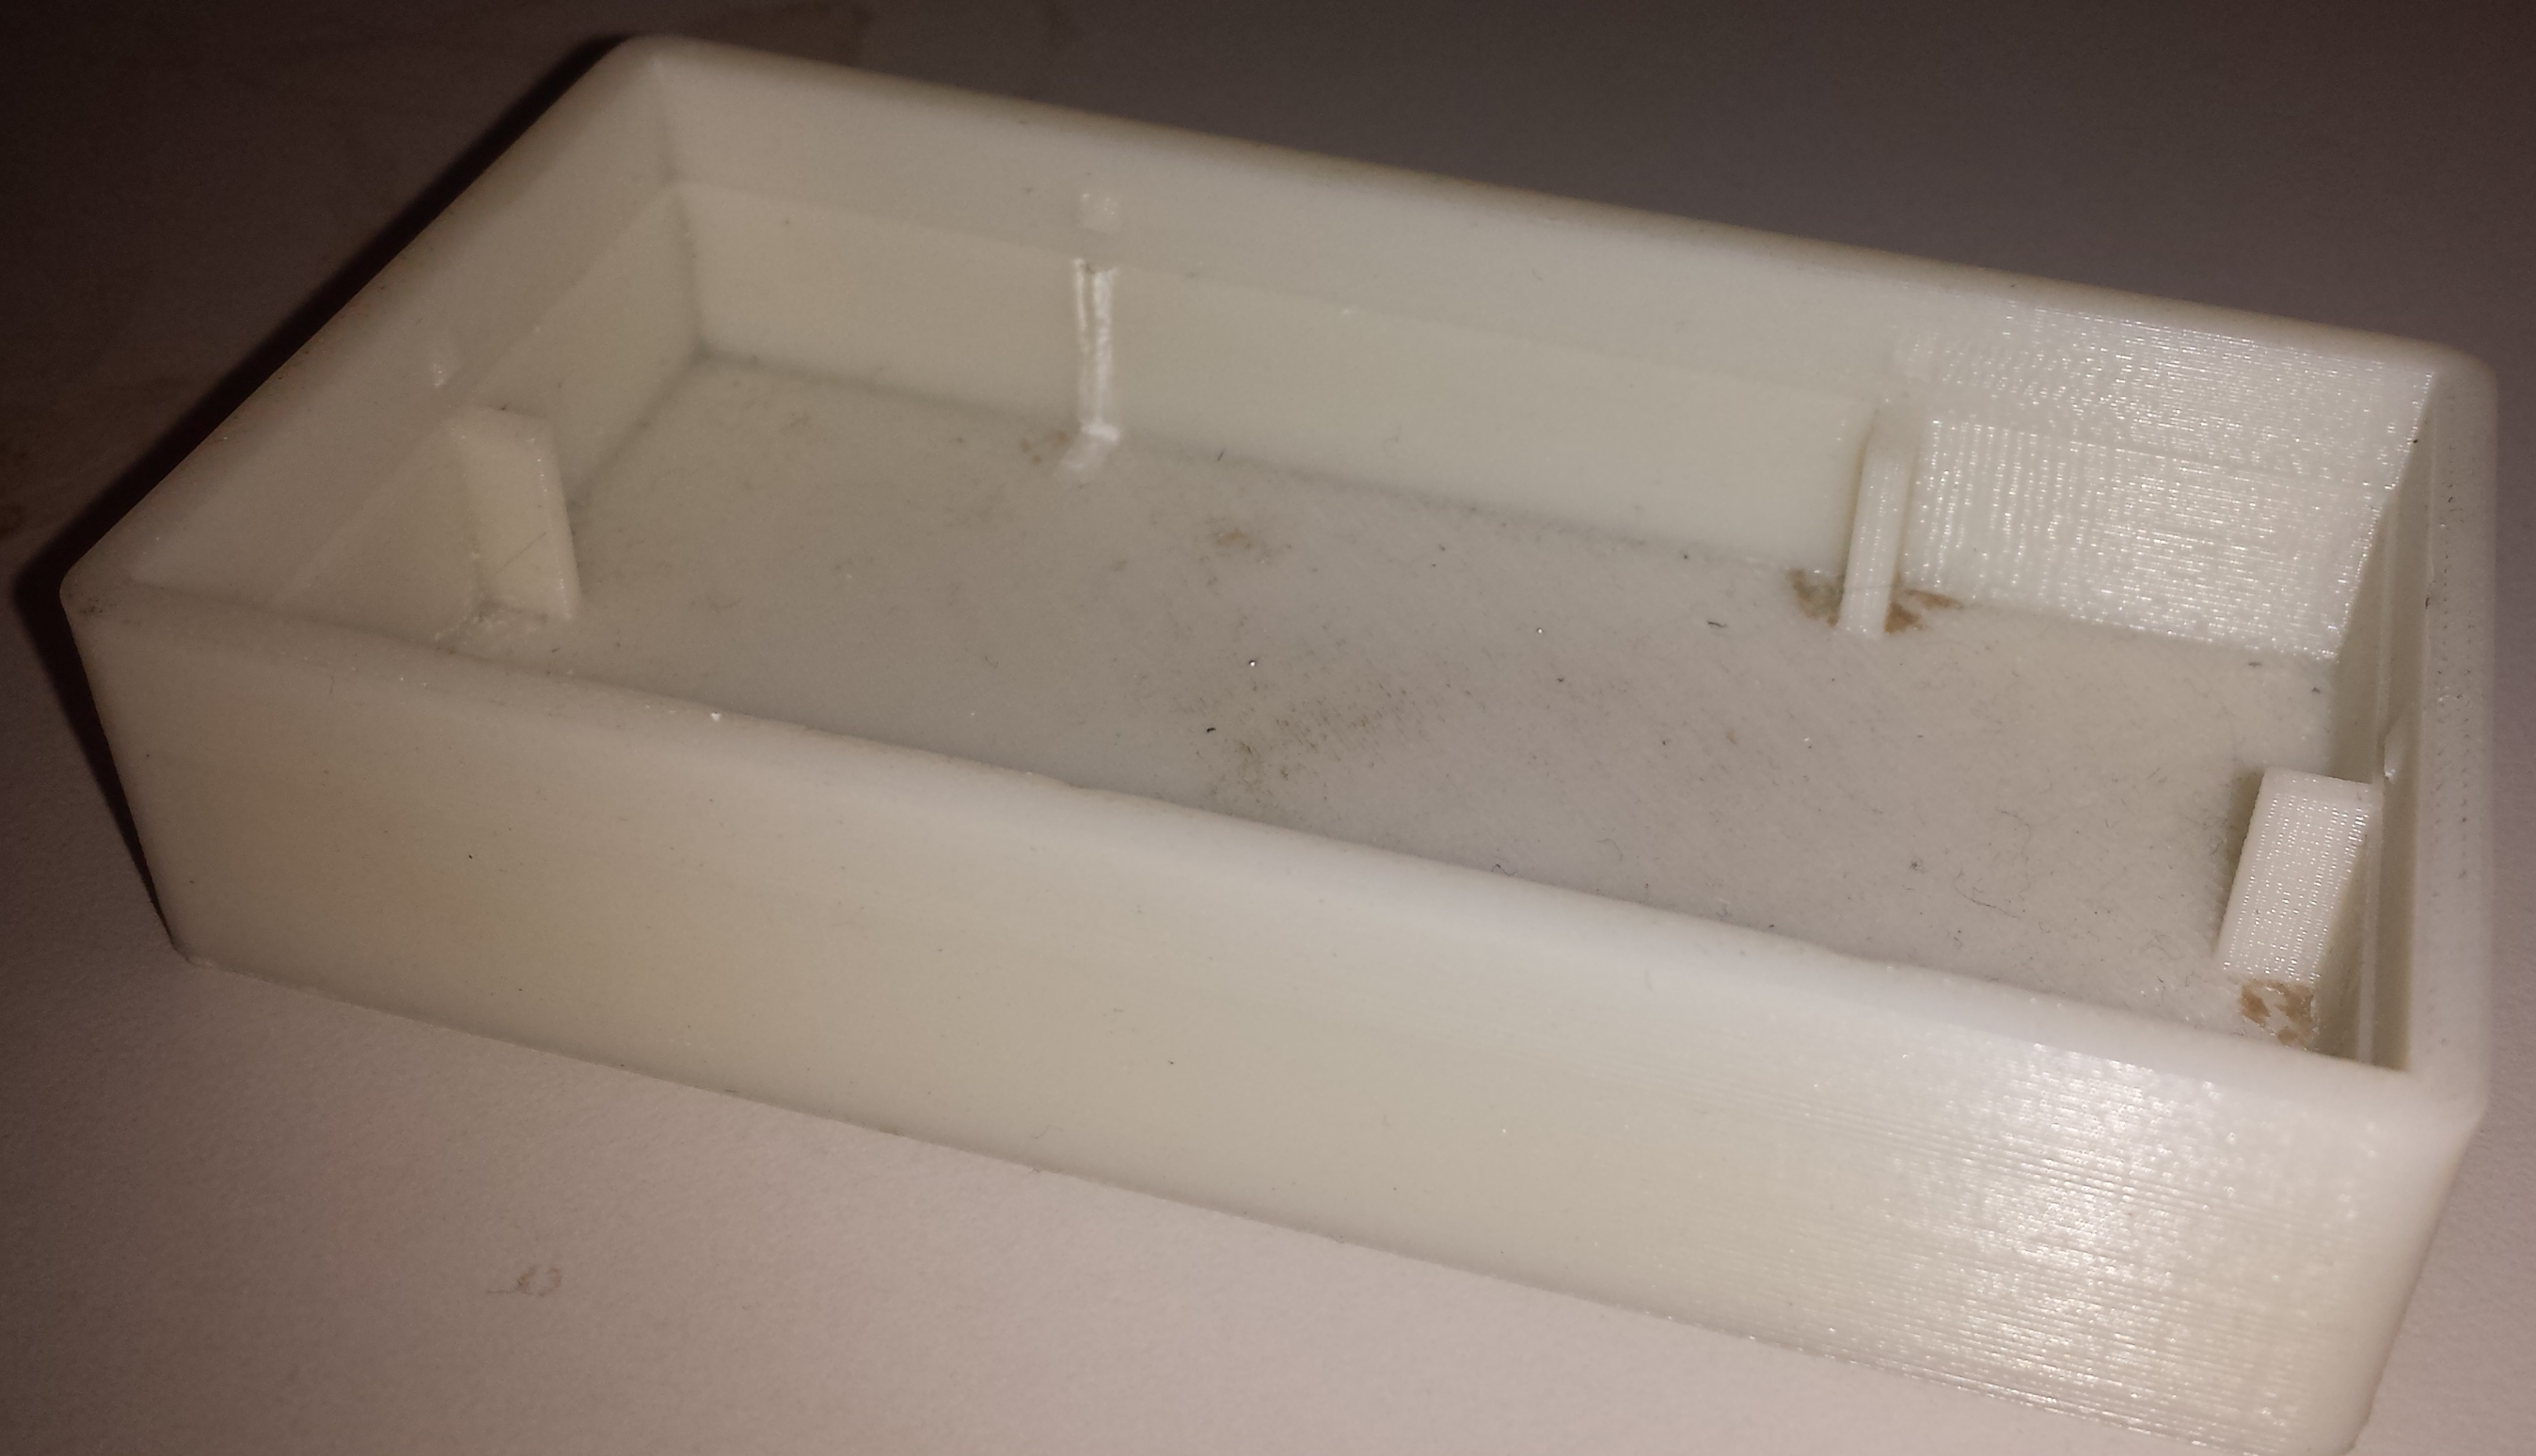
\includegraphics[scale=1,width=0.8\textwidth]{Images/Enclosure1.png} 
  \caption{Enclosure Rev 1, with Cut Tabs}
  \label{fig:enclosure1}
 \end{center}
\end{figure}


The next prototype stage moved the PCB standoffs, added ports for the USB, SD card, \spo2, and ECG connectors. It also smoothed out not only the four vertical edges of the enclosure but rounded all four bottom edges as well. A cover was also printed to completely enclose the electronics. A portion of the cover was designed to prevent warping, but reduce overall plastic use, as a structural precaution. This prototype worked well, allowing relatively easy removal of the PCB while still holding the board tight, however the SD card slot was not large enough to allow a thumb or finger to trigger the ejection mechanism for the card. The cover functioned well, but only after a section of the cover was removed to provide space for the programming header.  A hot knife was used, in each case, to remove plastic until the desired form was achieved, then calipers were used to measure the effected areas and the 3d model updated to reflect the new measurements.
\begin{figure}[ht]
 \begin{center}
  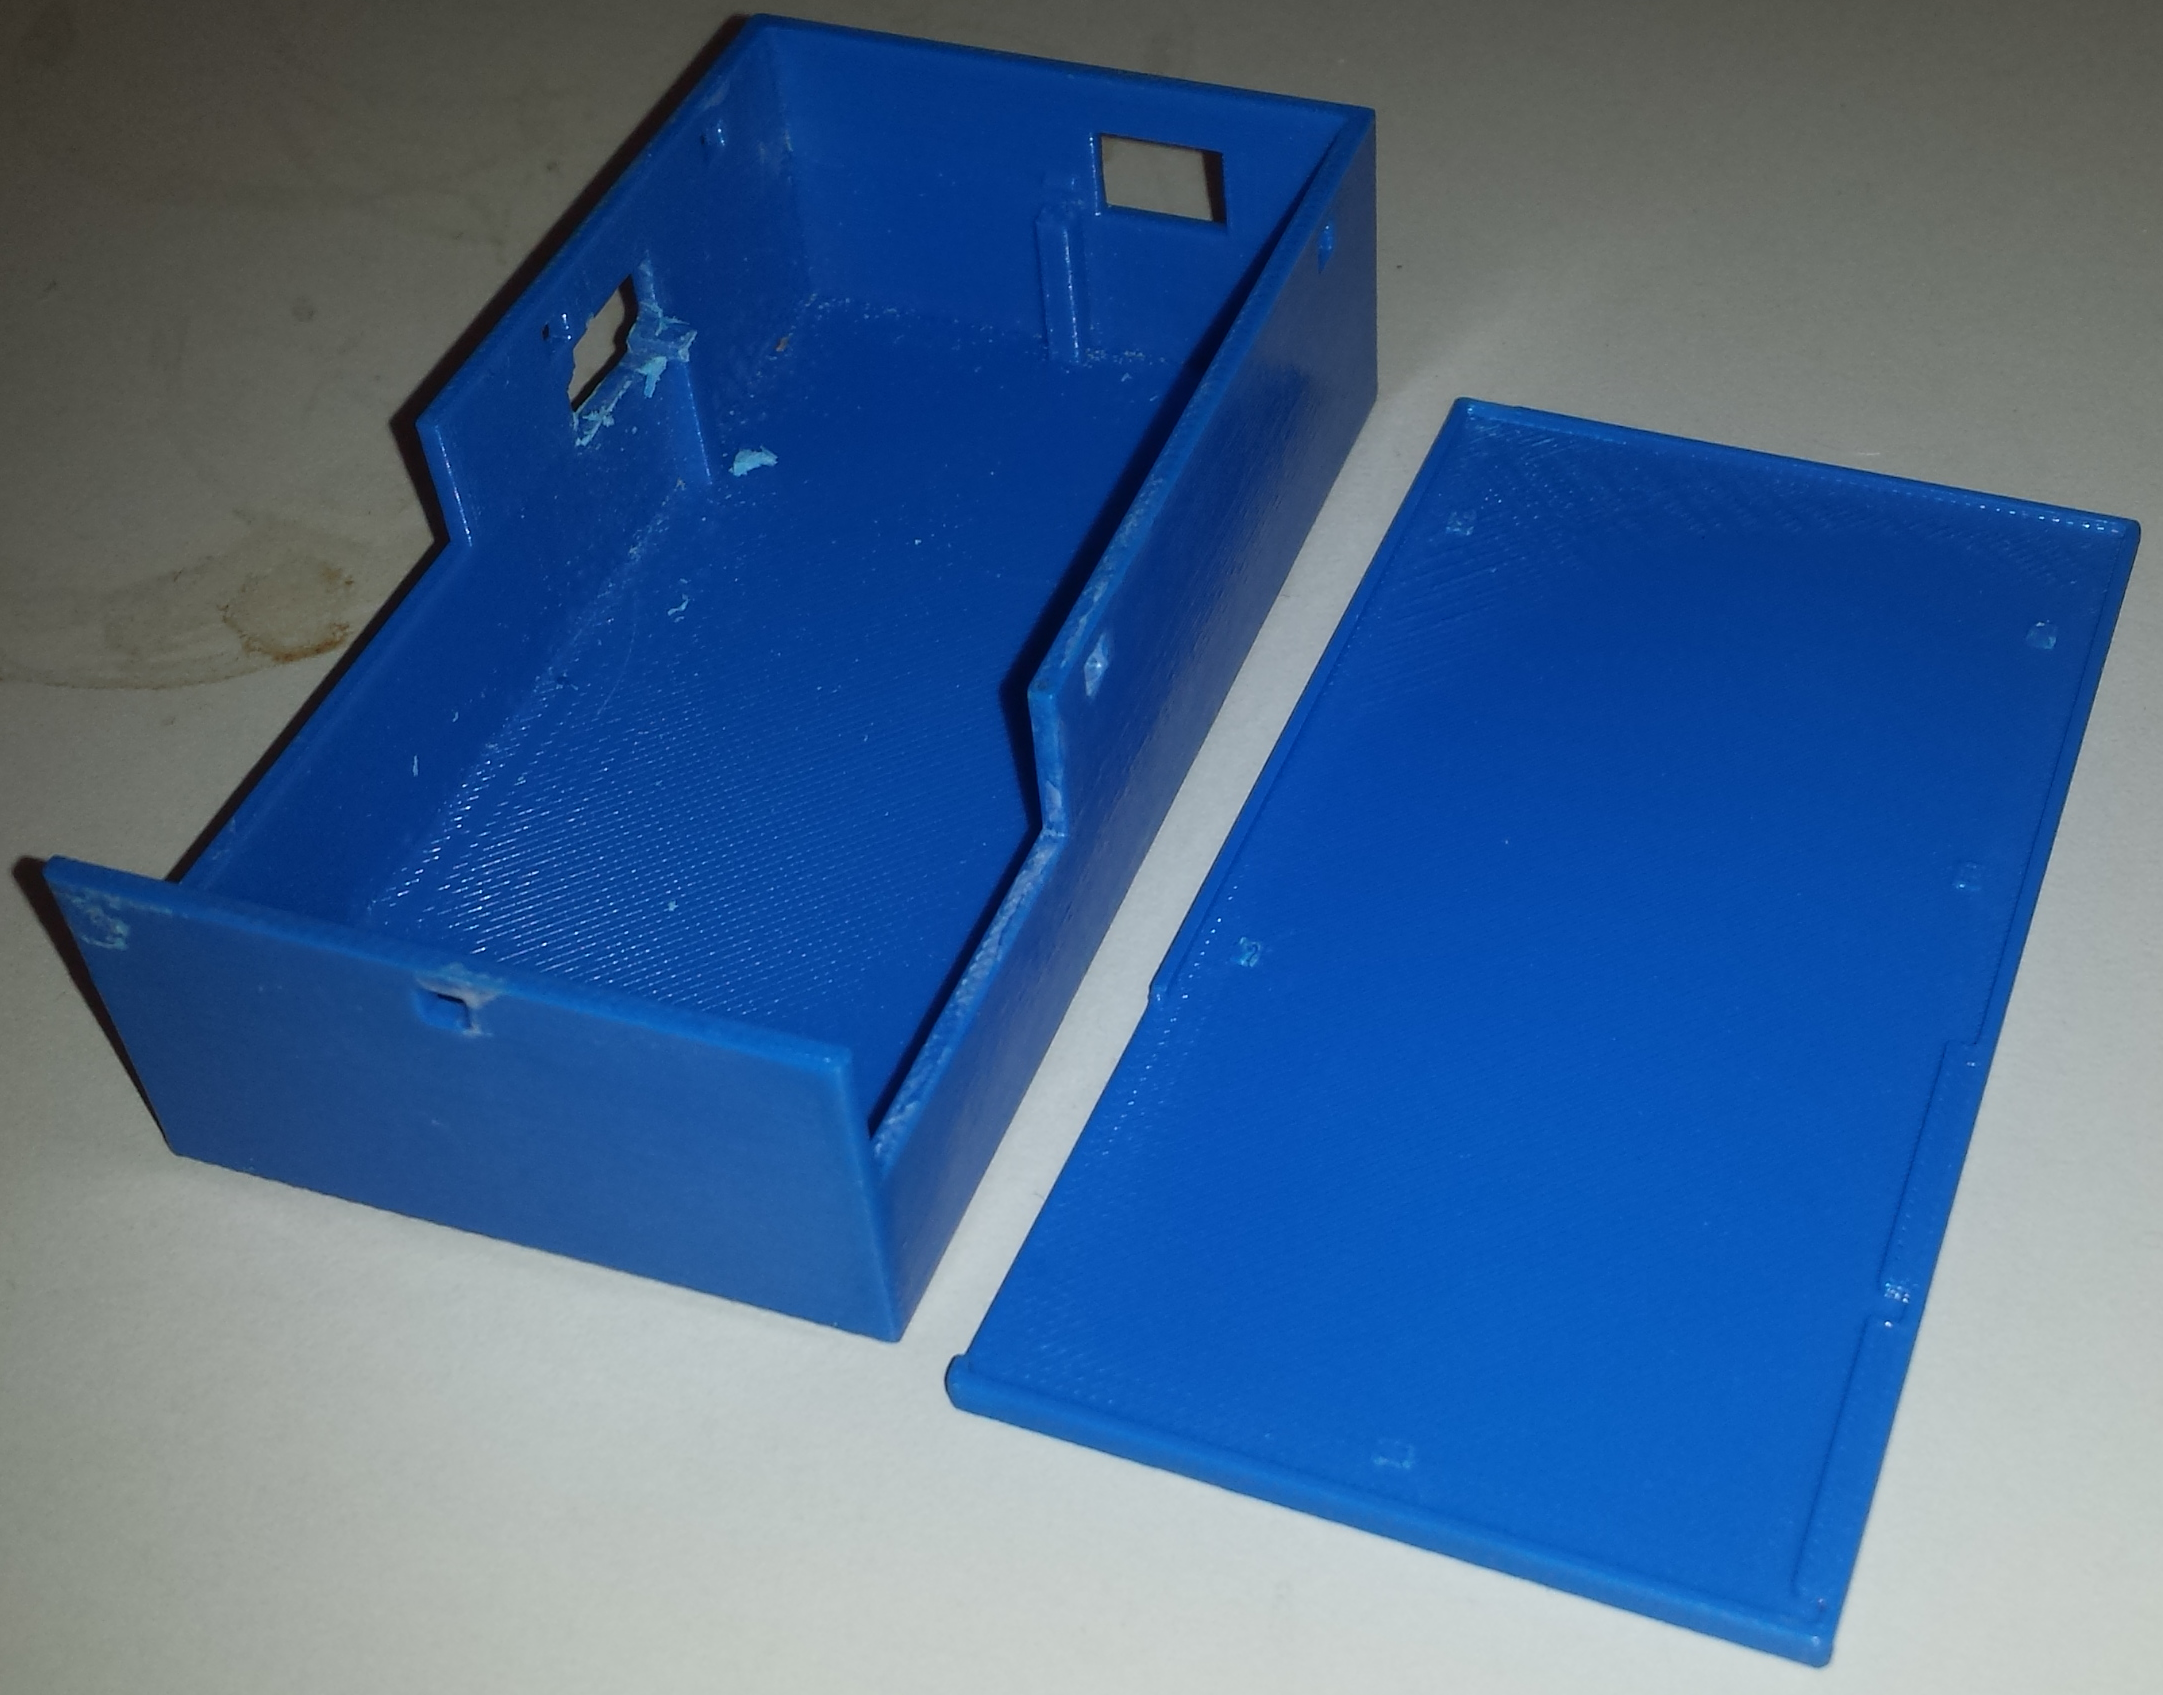
\includegraphics[scale=1,width=0.8\textwidth]{Images/Enclosure2.png} 
  \caption{Enclosure Rev 2, with Enlarged SD Slot}
  \label{fig:enclosure2}
 \end{center}
\end{figure}


It was at this point in the design process that the polar heart rate strap was introduced. The next prototype moved the ECG connection port from the side of the device to the bottom. A small insert was fabricated to fit into the model to allow it to snap directly to the polar strap. This model was printed and again modified to make channels for the wires that would connect from the snaps to the PCB. As shown in \Cref{fig:enclosure3} the enclosure was actually modified twice, the first time the modifications were made while the enclosure was upside down, which brings to mind the old adage ``measure twice, cut once''. 

\begin{figure}[ht]
 \begin{center}
  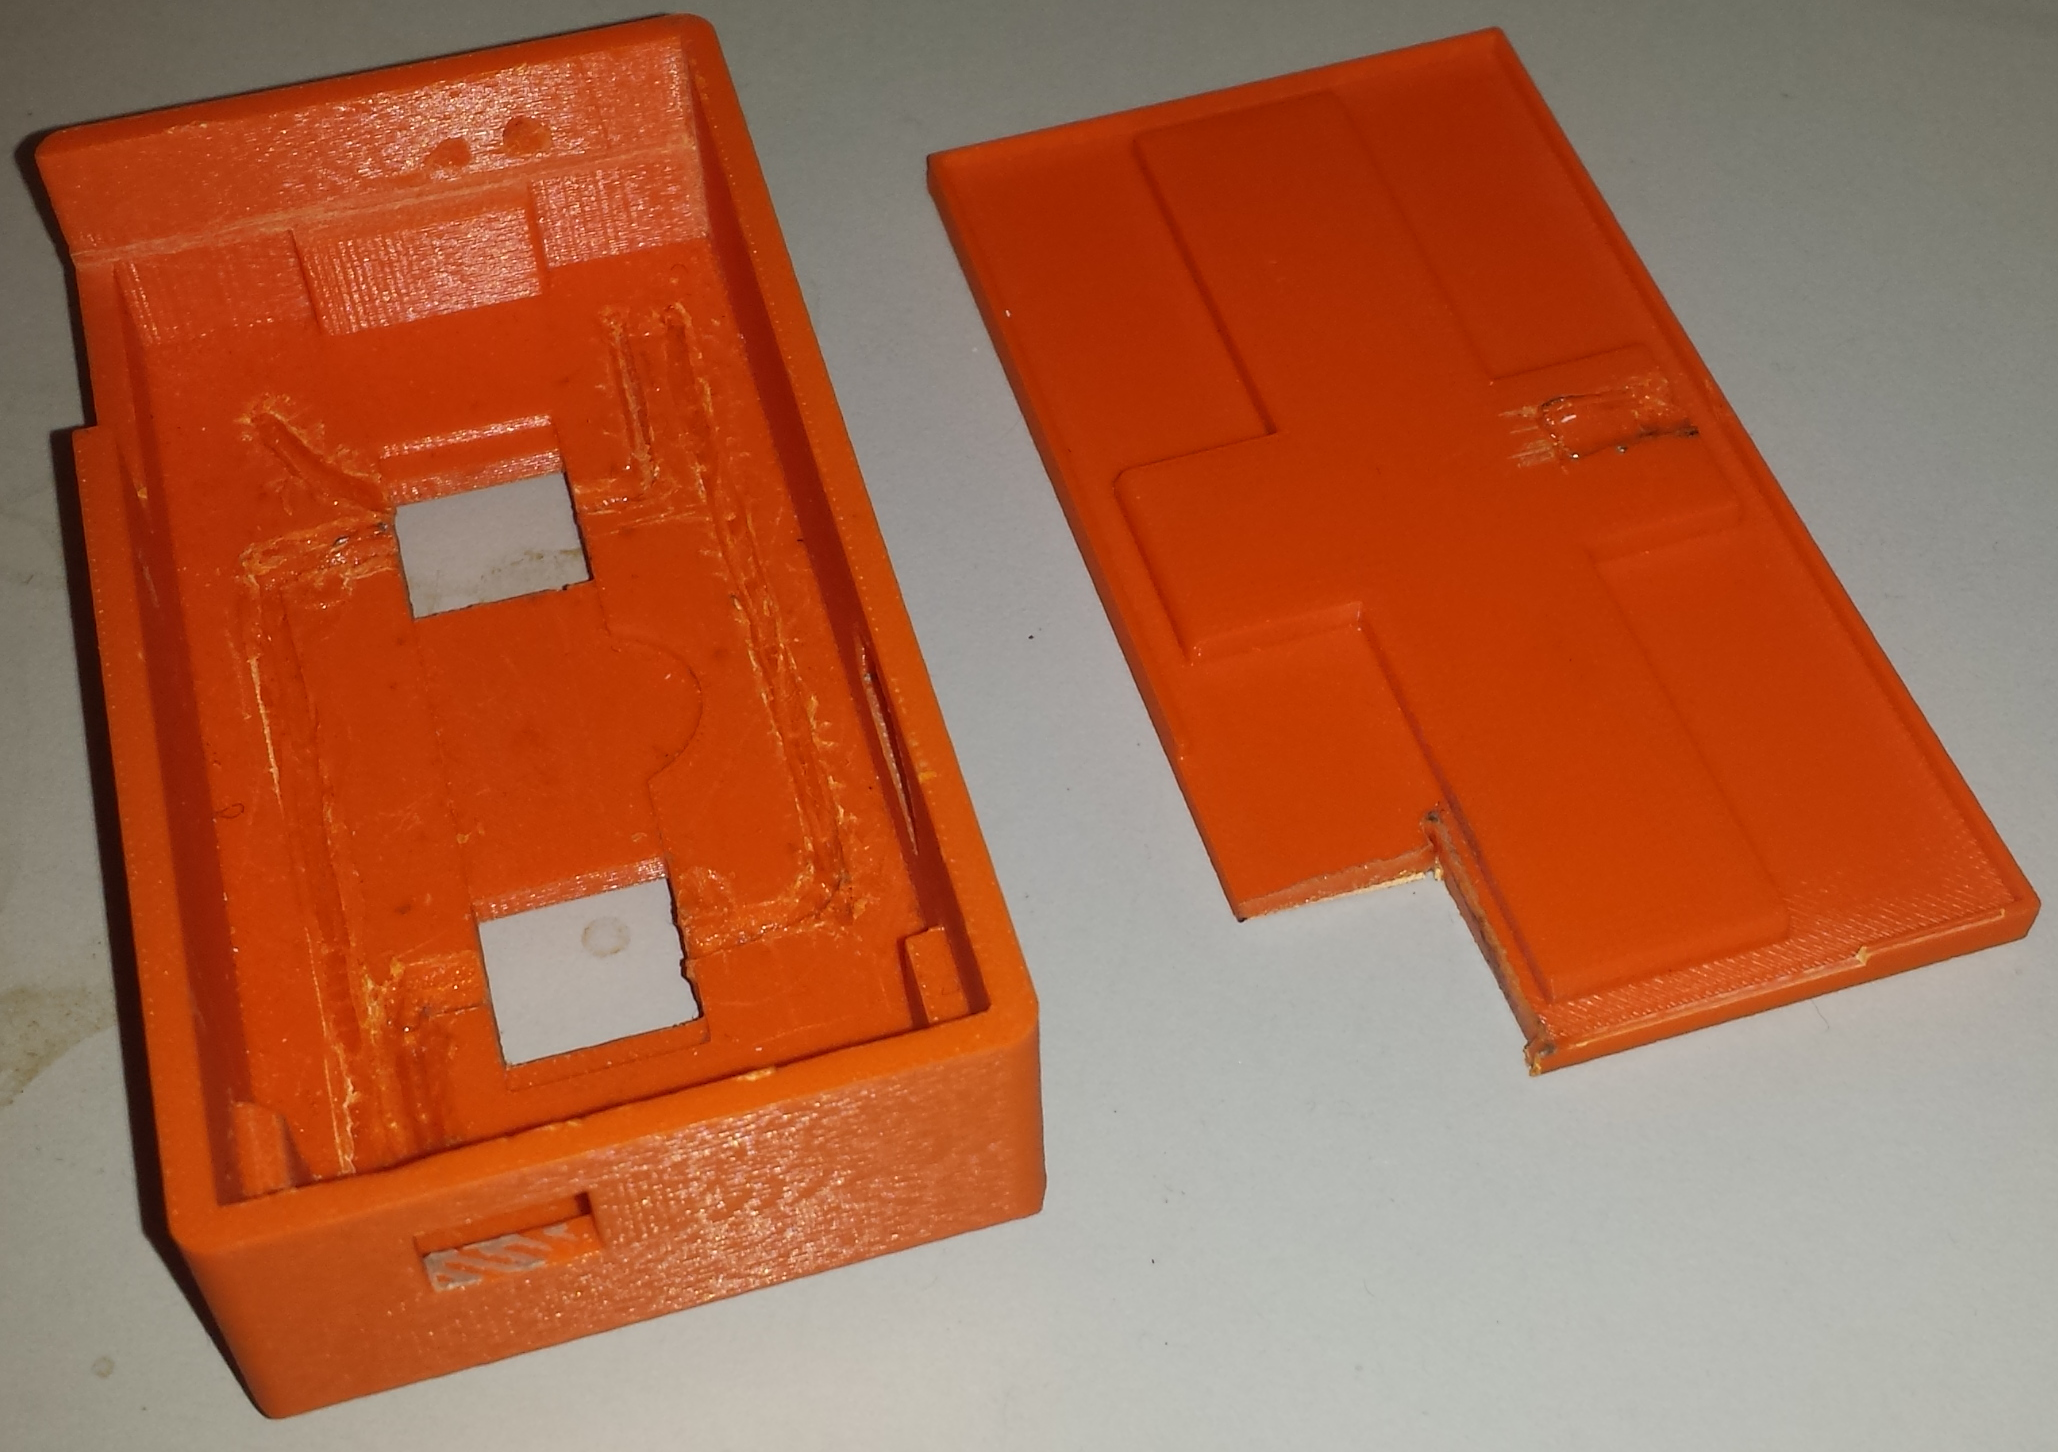
\includegraphics[scale=1,width=0.8\textwidth]{Images/Enclosure3.png} 
  \caption{Enclosure Rev 3, with Wire Management Trenches} 
  \label{fig:enclosure3}
 \end{center}
\end{figure}


The last enclosure integrates all the lessons learned in the previous designs, adding an extra aperture for the 3rd lead of the ECG. this design was printed multiple times for distribution during the study. The last modification to the enclosure was to put the entire device inside of a fabric pouch. The fabric was deemed more comfortable than the 3d printed plastic. Each fabric pouch was hand sewn and holes for the charging port and ECG leads were cut by hand. A hole for the SD card was not cut in the fabric to prevent accidental ejection during use. The fully constructed Enclosure is shown in \Cref{fig:enclosure4}.

\begin{figure}[ht]
 \begin{center}
  \includegraphics[scale=1,width=0.8\textwidth]{Images/Enclosure4.png} 
  \caption{Production Enclosure, with PCB and Battery} 
  \label{fig:enclosure4}
 \end{center}
\end{figure}

\subsection{Enclosure Conclusions}
3d printing was used to great effect in the enclosure design. The ability to modify a physical prototype provided the flexibility to just try design concepts on a whim. Since cost and risk are usually proportional in a design environment the extreme low cost of 3d printing, approximately two dollars and two hours per enclosure, provided a large amount of freedom to try out many designs before settling on a final implementation. Additionally, the ability to modify each prototype to add features allowed for instant feedback on each 3d model. 

The largest drawback to 3d printing each case was the time involved, and the rate of failure. The 3d printer was a new tool at the start of this process. Unfortunately it is not as user friendly as a traditional 2d laser printer. Going from model to printed object is not as simple as hitting ``print''. An additional step, know as Computer Aided Manufacturing (CAM), is required to turn the 3d model into movement instructions for the printer. This process is extremely flexible, however the flexibility provided by the process also introduces complexity. Additionally, to ensure reliable prints some preparation to the print bed is required. This was not immediately apparent, however once the problem was identified the rate of failure went from four out of five (80\%) to one in fifty (2\%). A 2\% failure rate may be considered high in bulk manufacturing, but for prototyping, it is acceptable.


\begin{figure}[ht]
 \begin{center}
  \includegraphics[scale=1,width=0.8\textwidth]{Images/Enclosure5.png} 
  \caption{Enclosure with Lessons Learned} 
  \label{fig:enclosure5}
 \end{center}
\end{figure}

\subsection{Enclosure Future Work}
In future research, it may be possible to speed prototyping time by using subtractive manufacturing techniques. Using acrylic sheets and a laser cutter a similar enclosure design could be fabricated in minutes instead of hours. Future designs may also introduce flexible PCB material that would allow a smaller volume of the overall enclosure. Finally, a curved enclosure design would more closely fit to the patients body increasing comfort. A final Enclosure was fabricated addressing some problems discovered during the experimental trial and some limitations of 3d printing. The enclosure shown in \cref{fig:enclosure5} can be 3d printed without overhangs or support material and does not present a lip on the enclosure cover. Additionally, the cover has been modified to protect the \spo2 connector from torsional forces during use.








\chapter{Embedded Software Concepts}
\label{chap:SensorConcepts}
%In this chapter, I will cover in detail the code and DSP techniques used in the data flow of the sensor designs covering both the analog front end for the real sensors and the software DSP and data fusion techniques for the synthetic sensors.
Any embedded design is a combination of both hardware and firmware. The WHIP is no different. The firmware was developed to allow for future expansion and should serve as a starting point, not an end point for development. All firmware was written in the C language. The development environment was Atmel Studio V6.2\cite{AtmelStudio}. The following sections cover the code generated for this firmware in the following groups. First the low level driver for the ECG and \spo2 chips; then the integration with the Atmel Software Framework and, finally, the driver code state machine

\begin{figure}
	\begin{center}
		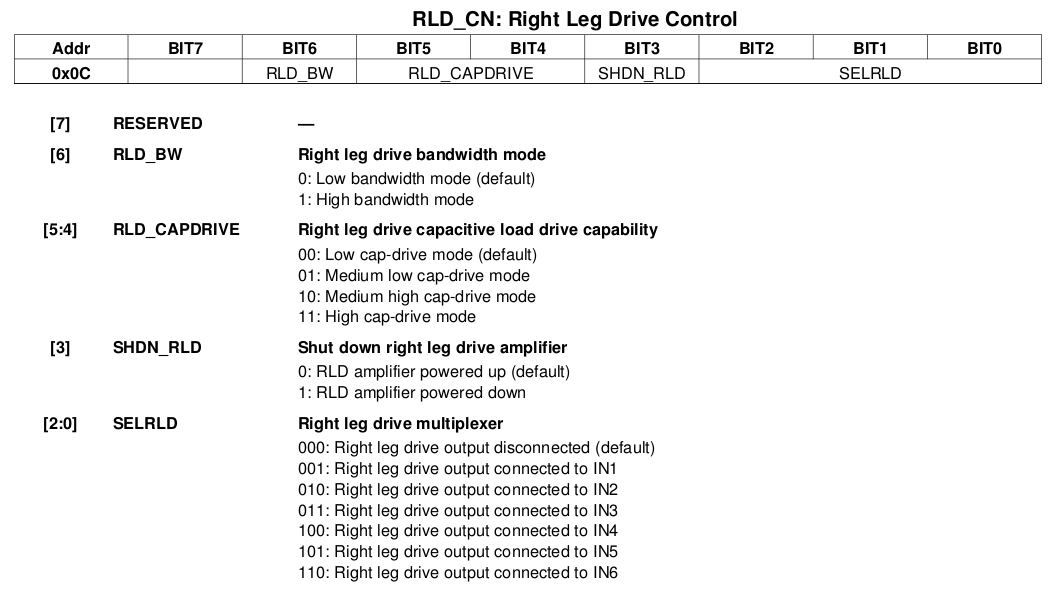
\includegraphics[scale=1,width=0.9\textwidth]{Images/ADS1293_RLD_CN_modified.png} 
		\caption{Excerpt from ADS1293 Data Sheet Describing the RLD CN Register}
		\label{fig:ADS1293_RLD_CN}
	\end{center}
\end{figure}

\section{Chip Driver Firmware}

Both the AFE4490 \spo2 IC and the ADS1293 ECG IC offered attractive features settable in software, including gain amplifiers and sample rate. However, these features, while flexible, required a substantial investment in understanding the configuration registers present in both chips. An intermediate C\# program was written to ingest specifications from the data sheet and produce a header file with descriptive \#define statements that could be used to create self-documenting code. Consider \Cref{fig:ADS1293_RLD_CN}, as an example, an excerpt from the ADS1293 data sheet shows a  bit-mapped register, responsible for several functions related to the right leg drive circuitry(RLD) of the ADS1293. The code in \cref{fig:ADS1293_Defines} was generated to simplify code generation and increase readability. The use of masking and bit shifting ensures that invalid bits do not unintentionally have side effects; and the descriptive bit names help document the code to communicate meaning. Examining the ADS1293 initialization routine in \Cref{fig:ADS1293_INIT} shows how effective this strategy can be. The use of a well organized array allows for all settings to be seen at a glance. This approach does not eliminate the need for the data sheet while programming, but by using define statements to create readable alternatives to hard coded binary numbers we greatly increase the maintainability of the code base. Both ICs received a similar treatment and a library of basic functionality was written for each chip.

\begin{figure}
	\begin{center}
\begin{lstlisting}[frame=single]
//RLD_CN
#define ADS1293_RLD_CN  0x0C

#define RLD_BW _BV(6)
#define RLD_CAPDRIVE(n) (((n)&3)<<4)
#define RLD_LOW_DRIVE 0
#define RLD_MED_LOW_DRIVE 1
#define RLD_MED_HIGH_DRIVE 2
#define RLD_HIGH_DRIVE 3
#define SHDN_RLD _BV(3)
#define SELRLD(n) (((n)&7)<<0)
\end{lstlisting}
		\caption{Self Documenting Define Statements for ADS1293 ``ADS1293.h''}
		\label{fig:ADS1293_Defines}
	\end{center}
\end{figure}


\begin{figure}
	\begin{center}
\begin{lstlisting}[frame=single,morekeywords={ECG_INIT_DATA}]
ECG_INIT_DATA ads1293Defaults[] = {
{ADS1293_FLEX_CH1_CN, POS(IN4)|NEG(IN5)}, 
{ADS1293_CMDET_EN,    CMDET(IN4)|CMDET(IN5)},
{ADS1293_CMDET_CN,    CMDET_BW | CMDET_HIGH_DRIVE},
{ADS1293_RLD_CN,      SELRLD(IN6)},
{ADS1293_AFE_SHDN_CN, SHDN_SDM(2)|SHDN_SDM(3)|
                      SHDN_INA(2)|SHDN_INA(3)},
{ADS1293_R2_RATE,     R2_RATE_4},
{ADS1293_R3_RATE_CH1, R3_RATE_8},
{ADS1293_R1_RATE,     R1_DOUBLE_CH1},
{ADS1293_DRDYB_SRC,   DRDYB_SRC_CH1ECG},
{ADS1293_MASK_DRDYB,  DRDYB_MASK_NONE},
{ADS1293_CH_CNFG,     E1_EN},
{ADS1293_OSC_CN,      STRTCLK|EN_CLKOUT},
{ADS1293_CONFIG,      START_CON}
};

void ECG_begin()
{
  for (int i=0;
       i<sizeof(ads1293Defaults)
         /sizeof(ads1293Defaults[0]);
         i++)
  {
    ECGsingleWrite(ads1293Defaults[i].address,
                   ads1293Defaults[i].data);
  }
}
\end{lstlisting}
		\caption{Initialization Code for ADS1293 ``ADS1293.c''}
		\label{fig:ADS1293_INIT}
	\end{center}
\end{figure}



\section{Atmel Software Framework (ASF)}
The Atmel website clearly sums up the ASF:

\begin{quotation}
The Atmel Software framework is a MCU software library providing a large collection of embedded software for Atmel flash MCUs: megaAVR, AVR XMEGA, AVR UC3 and SAM devices.

It  simplifies the usage of microcontrollers, providing an abstraction to the hardware and high-value middlewares
ASF is designed to be used for evaluation, prototyping, design and production phases
ASF is integrated in the Atmel Studio IDE with a graphical user interface or available as standalone for GCC, IAR compilers
ASF can be downloaded for free. \cite{AtmelStudio}
\end{quotation} 
% http://www.atmel.com/tools/avrsoftwareframework.aspx)

The two primary benefits to this project, provided by the ASF are its abstraction layer across different hardware devices, and its collection of embedded libraries.

Over the course of development several processors were used. All devices were manufactured by Atmel, but spanned different chip families. Early development used the megaAVR series of 8 bit processors, while the final design used the 32 bit UC3 series. The details of accessing the low level configuration registers of any specific hardware were ``hidden'' from the functional code by utilizing the ASF. The word ``hidden'' is in quotes because, often the low level code had to be rewritten by the programmer. But, this was well worth the time invested to keep the higher level libraries unchanged. Specifically, the SD card/FAT libraries allowed for a POSIX file interface to simplify sample storage, and the USB libraries made interfacing to a computer trivial; allowing the programmer to focus on interfacing with the relevant sensors and not on timing details of the USB specification.

\section{Main State Machine}

The basic state machine of the WHIP firmware, shown in \cref{fig:flowchart_main}, was simplistic, but robust. Data was pipelined directly from both ECG and \spo2 devices to a double buffered memory location By making use of the DMA channels on the micro controller . Then, another DMA channel wrote the collected data to the SD card. The CPU only intervened once the write-buffer was filled, at which point the buffers were swapped. The only other mode the device can enter is USB mode. Upon connection to USB power data collection is halted and all files are flushed and closed in preparation for download. When USB power is removed, data collection starts again. 

\begin{figure}
	\begin{center}
		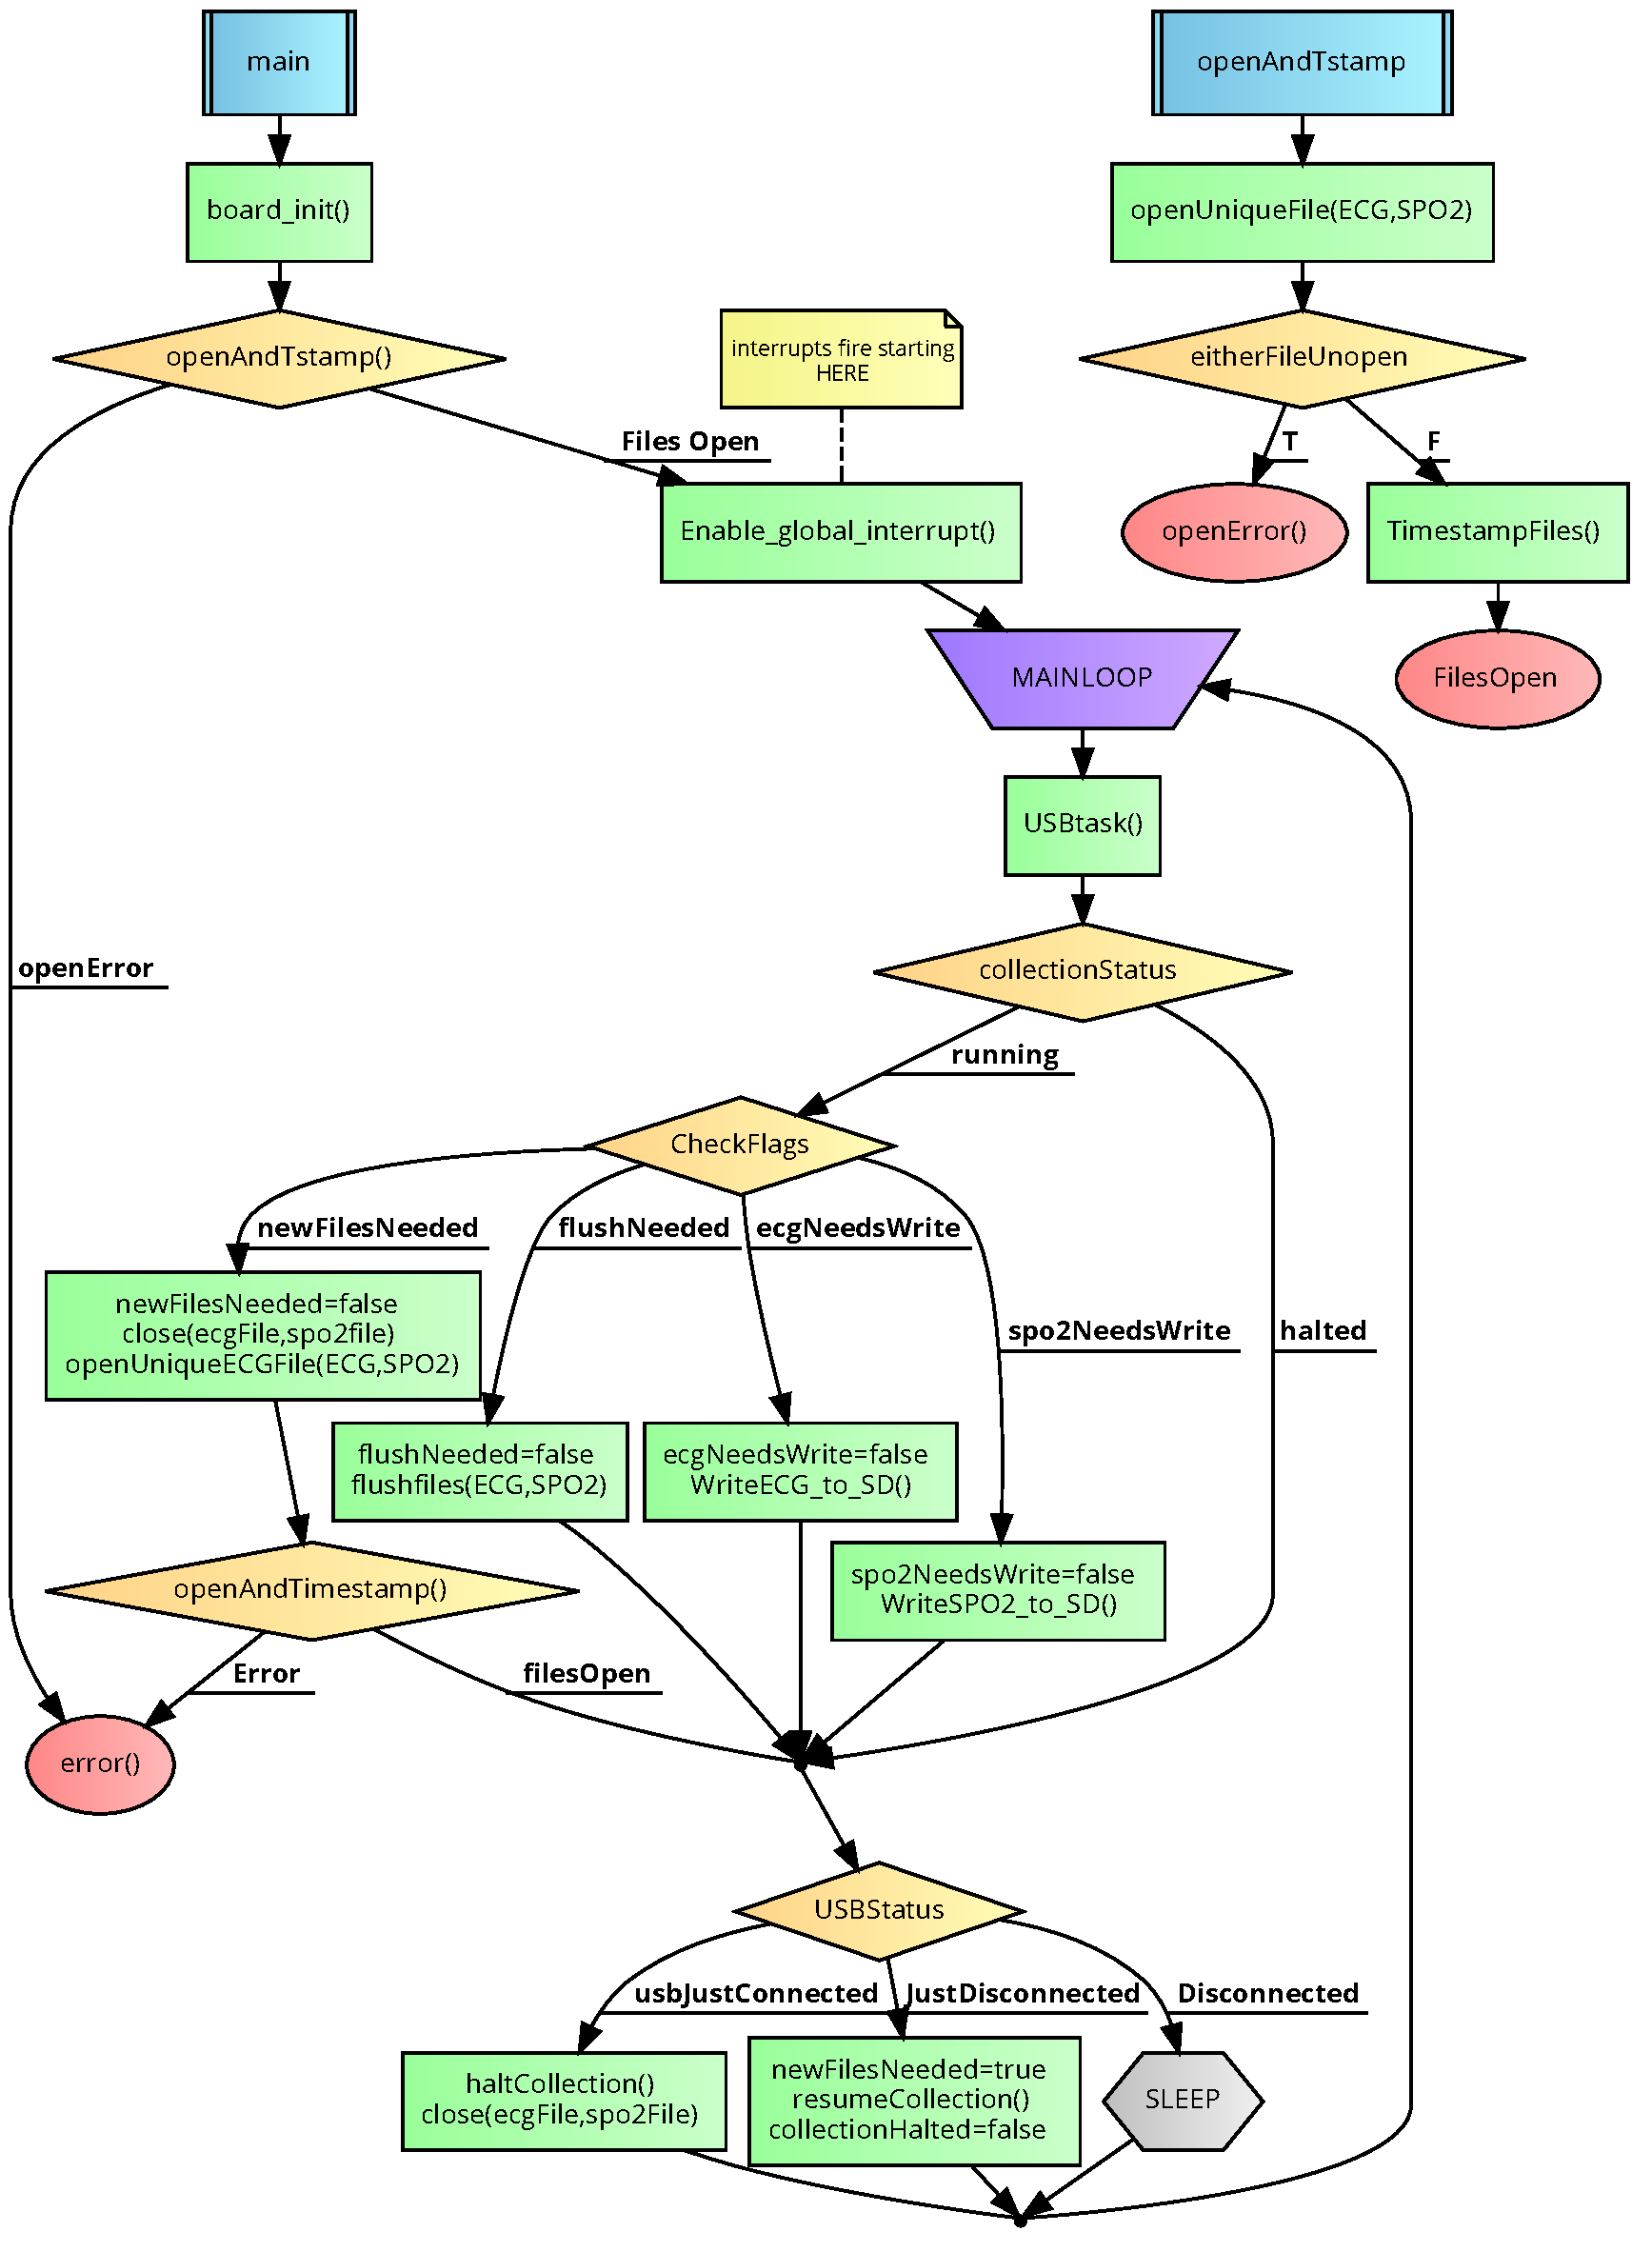
\includegraphics[scale=1,width=0.9\textwidth]{Images/FlowChartMain.pdf} 
		\caption{Main Function, Functional Flowchart}
		\label{fig:flowchart_main}
	\end{center}
\end{figure}

\section {Interrupt Service Routines (ISRs)}
Microcontrollers best utilize resources when not polling, using busy loops, waiting for events to occur. Interrupt Service Routines (ISRs) allow for low level tasks to be interrupted in favor of higher priority tasks. The ATUC3 line of microcontrollers offers many Interrupt sources. The two most important, from a WHIP firmware standpoint, are the Data Received interrupts for the AFE4490 \spo2 and the ADS1293 ECG chips. \cref{fig:flowchart_ISR} shows that both interrupts are similar. Both buffer incoming data until the buffer is full. When a buffer is full, a new buffer is swapped into place and the old buffer can be sent to the SD card for storage. The \spo2 interrupt contains one extra feature; a dynamic brightness calibration to prevent saturation of the pleth sensor. Other differences in the \spo2 ISR are not additional features just a reflection of the data delivered by the pleth sensor, two channels of data, and an additional two channels of intensity data.
\begin{figure}
	\begin{center}
		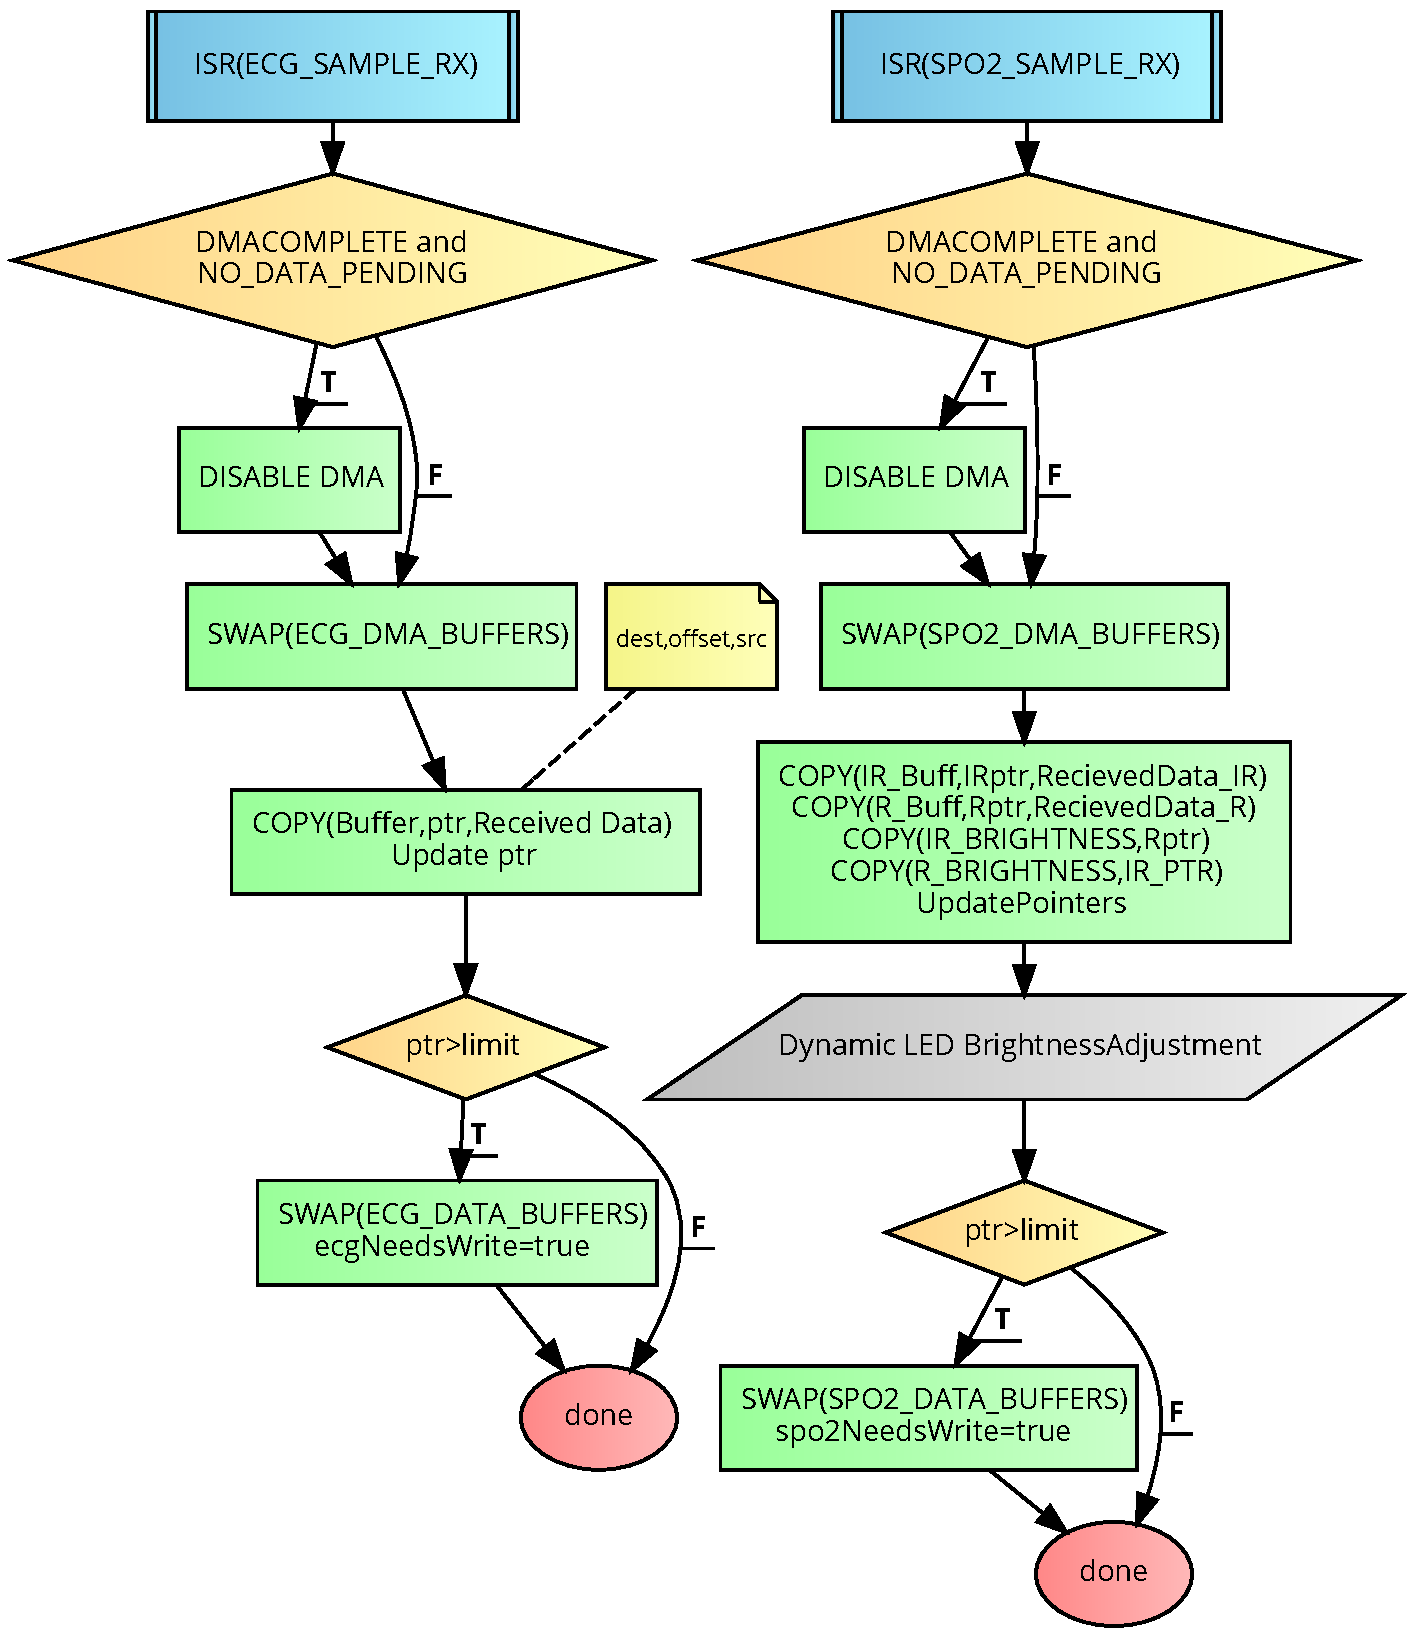
\includegraphics[scale=1,width=0.9\textwidth]{Images/FlowChartISR.pdf} 
		\caption{ISR Functional Flowchart}
		\label{fig:flowchart_ISR}
	\end{center}
\end{figure}


\chapter{Conclusions and Future Work}
\label{chap:conclusions}
%Validating my system with an exploratory study is only the first step in a larger design philosophy. I will indicate avenues of improvement for hardware and software focusing on moving to a system on a chip (SoC) design. I will present my conclusions and suggest future steps in the research.

%What Else? form fit issues
% what did the dissertation provide as a fundamental benifit?
% what else should be done, such as shrink all electrodes down to a physical patch.
%look more into spo2 Reflective designs.
\begin{figure}
\centering
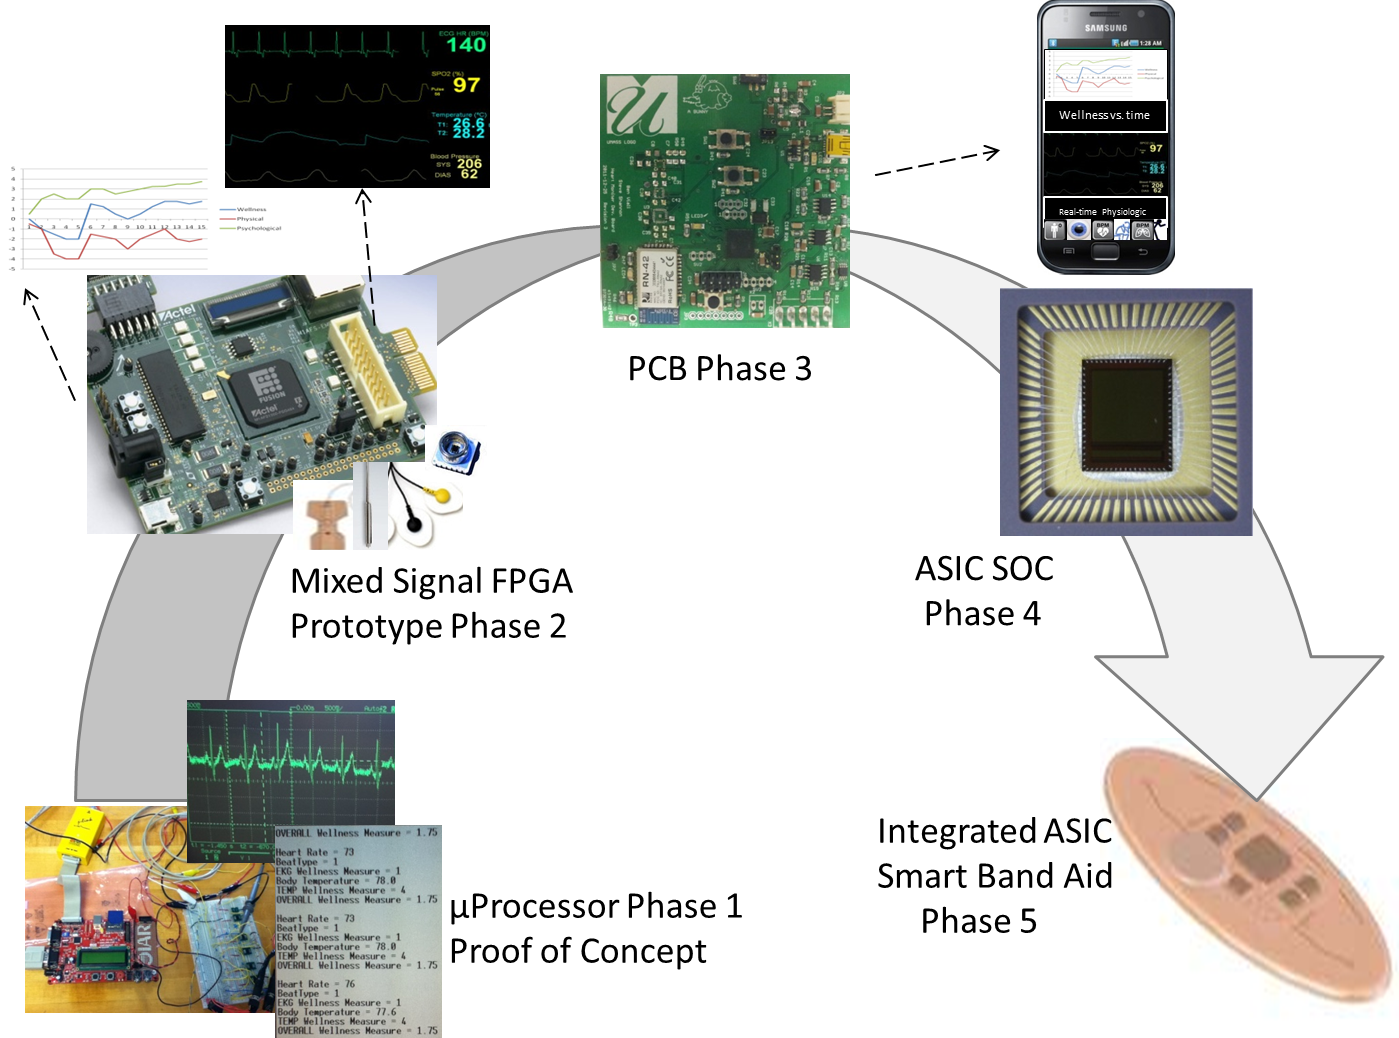
\includegraphics[width=0.7\linewidth]{Images/projectPhases}
\caption{Project Phases}
\label{fig:projectPhases}
\end{figure}


Throughout the process of this dissertation research new findings were always being rolled into the existing framework. The hardware platform for the WHIP sensor was developed from January to May 2014 . This design acquitted itself well through the entire process of the following trial. While some of its functions were under utilized (i.e.\ the Bluetooth communications) the platform demonstrates an ability to serve as a platform for future research with the ability to support more accurate ECG readings, different \spo2 measuring devices such as nasal alar sensors, and as demonstrated good low power design capabilities. 

A major limitation in the adoption of such a device is a physical constraint not a technological one. The device may be split into smaller modules in future iterations, to more closely contour the human body. This will not be a change to the design of the device, merely a dividing of the modules into different physical PCBs. One approach to increasing adoption of a WHIPPED-like system is to reduce its overall size. Given the work in miniaturizing the various analog front ends\cite{AFE4490,ADS1293}, this design could be miniaturized with appropriate manufacturing support to a disposable patch as proposed in \cref{fig:projectPhases}. The miniaturization of the WHIP sensor would necessitate some fundamental changes in the system design. Foremost, the \spo2 sensor would need to be switched from a transmittance sensor to a reflective sensor. Some preliminary work was done, investigating the integration of a reflective sensor into the design but was abandoned due to time. The sample sensor prototype was designed from the ground up , designed to be as flat as possible. A sensor such as the one shown in  \cref{fig:ReflectiveSensorPrototypes} would then need to be integrated into the sensor strap, or sensor patch.

\begin{figure}
\centering
\includegraphics[width=0.5\linewidth]{Images/ReflectiveSensorPrototype.png}
\caption{Reflective Sensor Prototype }
\label{fig:ReflectiveSensorPrototypes}
\end{figure}


The Cellphone was effective at conveying somatic surveys to patients and allowing them to upload information. Future work may include studies on effective user interface choices to simplify the process for patients unfamiliar with cellphone technologies. One problem with the current cell phone approach is updating the surveys during studies, improving the smartphones ability to procure data from a centralized source will make survey maintenance easier in future studies.

In this dissertation, a new sensor platform was developed and tested on a representative heart failure population. The WHIPPED system has been validated as a data gathering tool. The smartphone application has seen continued usage in other studies. The WHIP sensor has shown promise as a platform for longterm data collection. The exploratory trial gave new insights into the potential for the WHIPPED end-to-end system by collecting feedback from patients that can be worked into future iterations of WHIPPED.







\addtocontents{toc}{\vspace{\parskip}} \vspace{\parskip}
% Beginning of back matter
\backmatter  %% <--- mandatory



%% A bibliography is required.
\interlinepenalty=10000  % prevent split bibliography entries
%\bibliographystyle{umthesis}
% downloaded the latest IEEE style from 
% http://www.dlsi.ua.es/wemis09/styles/IEEEtran.bst
% and put it in the project directory. called it myieeetrA.bst
\bibliographystyle{myieeetrA}
\addcontentsline{toc}{chapter}{Bibliography}
%\chapter{Bib}
\bibliography{Draft1}


\begin{appendices}
%patch the apendix header thing to center shit % % % % % % % % % % % %
\apendixStyle
% End patch of apendix % % % % % % % % % % % % % % % % % % % % % % % % %
\appendix
\renewcommand{\cftchappresnum}{Appendix }
\chapter{PCB Schematics}
%\addcontentsline{toc}{chapter}{ WHIP Schematics }
\label{chap:PCB_Schematics}
\begin{figure}
	\begin{center}
		\label{fig:FullSchematic_Sheet1}
		\includegraphics[angle=90,scale=1,width=1\textwidth]{Images/rev1D_sheet1.pdf} 
		\caption{Full Schematic, Microprocessor View}
	\end{center}
\end{figure}

\begin{figure}
	\begin{center}
		\label{fig:FullSchematic_Sheet2}
		\includegraphics[angle=90,scale=1,width=1\textwidth]{Images/rev1D_sheet2.pdf} 
		\caption{Full Schematic, Bluetooth, Power System, and SD Card View}
	\end{center}
\end{figure}

\begin{figure}
	\begin{center}
		\label{fig:FullSchematic_Sheet3}
		\includegraphics[angle=90,scale=1,width=1\textwidth]{Images/rev1D_sheet3.pdf} 
		\caption{Full Schematic, \spo2 View}
	\end{center}
\end{figure}

\begin{figure}
	\begin{center}
		\label{fig:FullSchematic_Sheet4}
		\includegraphics[angle=90,scale=1,width=1\textwidth]{Images/rev1D_sheet4.pdf} 
		\caption{Full Schematic ECG View}
	\end{center}
\end{figure}

\chapter{PCB LAYOUT}
%\addcontentsline{toc}{chapter}{ WHIP Layout }
\label{chap:PCB_LAYOUT}

\begin{figure}
\begin{center}
	\label{fig:TOPGerber}
	\includegraphics[angle=0,scale=1,width=.8\textwidth]{Images/Rev5_TOPGERB.png} 
	\caption{Gerber Render for Top Layer}
\end{center}
\end{figure}


\begin{figure}
\begin{center}
	\label{fig:BOTGerber}
	\includegraphics[angle=0,scale=1,width=.8\textwidth]{Images/Rev5_BOTGERB.png} 
	\caption{Gerber Render for Bottom Layer}
\end{center}
\end{figure}


\begin{figure}
\begin{center}
	\label{fig:GNDGerber}
	\includegraphics[angle=0,scale=1,width=.8\textwidth]{Images/Rev5_GNDGERB.png} 
	\caption{Gerber Render for Internal Ground Layer}
\end{center}
\end{figure}


\begin{figure}
\begin{center}
	\label{fig:PWRGerber}
	\includegraphics[angle=0,scale=1,width=.8\textwidth]{Images/Rev5_PWRGERB.png} 
	\caption{Gerber Render for Internal Power Layer}
\end{center}
\end{figure}


\chapter {Institutional Research Board (IRB) Material}
\section{Permission Letter}
\fbox{\includegraphics[trim= 0mm 20mm 0mm 20mm,clip,page=1,width=\textwidth]{Images/IRB_Form.pdf}}
%had to mess with scale and offsett a zillion times to get it to fit in the margins
\includepdf[offset= .3in 0in, frame,trim= 0mm 20mm 0mm 20mm,clip, pages={2-5},width=\textwidth]{Images/IRB_Form.pdf}
\includepdf[offset= .3in 0in,frame,trim= 0mm 35mm 0mm 20mm,clip, pages={6-},width=\textwidth]{Images/IRB_Form.pdf}


\section{Duke Activity Status Index} 
\fbox{\includegraphics[page=1,width=.95\textwidth]{Images/DASI_form.pdf}}

\section{Heart Failure Somatic Awareness Scale}
\fbox{\includegraphics[page=1,angle=90,width=.95\textwidth]{Images/HFSA_Form.pdf}}

\noindent Continued on Next Page

\section*{Heart Failure Somatic Awareness Scale (cont.)}
\noindent\fbox{\includegraphics[page=2,angle=90,width=.95\textwidth]{Images/HFSA_Form.pdf}}

\noindent Continued on next Page

\section*{Heart Failure Somatic Awareness Scale (cont.)}
\noindent\fbox{\includegraphics[,page=3,angle=90,width=.95\textwidth]{Images/HFSA_Form.pdf}}

%\cftaddtitleline{toc}{chapter}{Source Code}{Back Pocket}
\chapter{Source Code: CD Back Pocket}

\end{appendices}


\end{document}
